\documentclass[11pt,a4paper,oneside]{book}
\usepackage[table]{xcolor}
\usepackage[utf8]{inputenc}
\usepackage{amsmath}
\usepackage{dsfont}
\usepackage{listings}
\usepackage{amsfonts}
\usepackage{amssymb}
\usepackage{tabularx}
\usepackage{booktabs}
\usepackage{enumitem}
\usepackage{algorithm}% http://ctan.org/pkg/algorithm
\usepackage[noend]{algorithmic}
\usepackage{parskip}
\usepackage{tikz}
\usepackage[margin=1in]{geometry}
\usepackage{graphicx}
\usepackage{hyperref}
\usepackage{epigraph}
\usetikzlibrary{arrows,fit,positioning}
\usepackage{subcaption}
\usepackage[colorinlistoftodos]{todonotes}
\usepackage[numbers]{natbib}
\usepackage{wrapfig}

% this is included to get tables with colored rows to not draw over hlines and vlines
\usepackage{etoolbox}

\makeatletter
\patchcmd{\@classz}
  {\CT@row@color}
  {\oldCT@column@color}
  {}
  {}
\patchcmd{\@classz}
  {\CT@column@color}
  {\CT@row@color}
  {}
  {}
\patchcmd{\@classz}
  {\oldCT@column@color}
  {\CT@column@color}
  {}
  {}
\makeatother


\usepackage{amsthm}

\graphicspath{ {figures/} }
\pgfarrowsdeclarecombine{ring}{ring}{}{}{o}{o}

\DeclareMathOperator{\ringarrow}{\raisebox{0.5ex}{\tikz[baseline]{\draw[ring->](0,0)--(2em,0);}}}
\DeclareUnicodeCharacter{00A0}{ }




\tikzset{
    %Define standard arrow tip
    >=stealth',
    %Define style for boxes
    punkt/.style={
           circle,
           rounded corners,
           draw=black, thick,
           text width=1em,
           minimum height=1em,
           text centered},
    observed/.style={
           circle,
           rounded corners,
           draw=black, thick,
           minimum width=2.2em,
           minimum height=2.2em,
           font=\footnotesize,
           text centered,
           fill=black!10!white
           },
     latent/.style={
           circle,
           rounded corners,
           draw=black, thick, dashed,
           minimum width=2.2em,
           minimum height=2.2em,
           font=\footnotesize,
           text centered
           },
    target/.style={
           circle,
           rounded corners,
           draw=black, thick,
           minimum width=2.2em,
           minimum height=2.2em,
           font=\footnotesize,
           text centered,
           fill=black!20!white,
           },
    observedrect/.style={
           rectangle,
           rounded corners,
           draw=black, thick,
           minimum width=6em,
           minimum height=2em,
           font=\footnotesize,
           text centered,
           fill=black!10!white
           },
    latentrect/.style={
           rectangle,
           rounded corners,
           draw=black, thick, dashed,
           minimum width=2.2em,
           minimum height=2.2em,
           font=\footnotesize,
           text centered
           },
     targetrect/.style={
           rectangle,
           rounded corners,
           draw=black, thick,
           minimum width=6em,
           minimum height=2em,
           font=\footnotesize,
           text centered,
           fill=black!20!white,
           },
     empty/.style={
           circle,
           rounded corners,
           minimum width=.5em,
           minimum height=.5em,
           font=\footnotesize,
           text centered,
           },
    % Define arrow style
    pil/.style={
           o->,
           thick,
           shorten <=2pt,
           shorten >=2pt,},
    sh/.style={ shade, shading=axis, left color=red, right color=green,
    shading angle=45 }   
}





\newcommand{\KL}{\operatorname{KL}}
\newcommand{\simpleregret}{R_T}
\newcommand{\Pij}[1]{\operatorname{P}_{ij}\!\left\{#1\right\}}
\newcommand{\Pkl}[1]{\operatorname{P}_{kl}\!\left\{#1\right\}}
\newcommand{\Q}[1]{\operatorname{Q}\left\{#1\right\}}
\newcommand{\EE}{\mathbb E}
\newcommand{\EEa}{\EE_a}
\newcommand{\Pns}[2]{\operatorname{P}_{#1}\left\{#2\right\}}
\newcommand{\Pn}[2]{\operatorname{P}\left\{#2|#1\right\}}
\newcommand{\actions}{\mathcal{A}}
\newcommand{\calA}{\mathcal A}
\newcommand{\etc}{\textit{etc}}
\newcommand{\ie}{\textit{i.e.}}
\newcommand{\eg}{\textit{e.g.}}
\newcommand{\calP}{\mathcal P}
\newcommand{\x}{\boldsymbol{x}}
\newcommand{\Ps}{\operatorname{P}}
\newcommand{\R}{\mathbb R}
\newcommand{\Pri}[1]{\operatorname{P}_i\left\{#1\right\}}
\newcommand{\Prz}[1]{\operatorname{P}_0\left\{#1\right\}}




\newcommand{\defined}{\vcentcolon =}
\newcommand{\rdefined}{=\vcentcolon}
\newcommand{\E}[1]{\mathbb E\left[{#1}\right]}
\newcommand{\Var}{\operatorname{Var}}
\newcommand{\calF}{\mathcal F}
\newcommand{\sr}[1]{\stackrel{#1}}
\newcommand{\set}[1]{\left\{#1\right\}}
\newcommand{\ind}[1]{\mathds{1}\!\!\set{#1}}
\newcommand{\argmax}{\operatornamewithlimits{arg\,max}}
\newcommand{\argmin}{\operatornamewithlimits{arg\,min}}
\newcommand{\floor}[1]{\left \lfloor {#1} \right\rfloor}
\newcommand{\ceil}[1]{\left \lceil {#1} \right\rceil}
\newcommand{\eqn}[1]{\begin{align}#1\end{align}}
\newcommand{\eq}[1]{\begin{align*}#1\end{align*}}
\newcommand{\Ber}{\operatorname{Bernoulli}}
\newcommand{\bigo}[1]{\mathcal{O}\left( #1 \right)}
\newcommand{\bigotilde}[1]{\tilde{\mathcal{O}}\left( #1 \right)}
\newcommand{\bigtheta}[1]{\Theta\left( #1 \right)}
\newcommand{\bigthetatilde}[1]{\tilde{\Theta}\left( #1 \right)}
\newcommand{\bigomega}[1]{\Omega\left( #1 \right)}

\renewcommand{\P}[1]{\operatorname{P}\left\{#1\right\}}
\newcommand{\cf}[2]{{#1}_{#2}}
\newcommand{\bernoulli}{\operatorname{Bernoulli}}
\newcommand{\dirac}{\operatorname{Dirac}}
\newcommand{\parents}[1]{\operatorname{\mathcal{P}a}_{#1}}
\renewcommand{\vec}[1]{\boldsymbol{#1}}

\theoremstyle{plain} 
\newtheorem{theorem}{Theorem}
\newtheorem{proposition}[theorem]{Proposition}
\newtheorem{lemma}[theorem]{Lemma}
\newtheorem{corollary}[theorem]{Corollary}

\theoremstyle{definition}
\newtheorem{definition}[theorem]{Definition}
\newtheorem{assumption}[theorem]{Assumption}
\newtheorem{remark}[theorem]{Remark}
\newtheorem{example}[theorem]{Example}
\let\temp\epsilon
\let\epsilon\varepsilon



\author{Finnian Lattimore}
\title{Learning how to act: making good decisions with machine learning}

\begin{document}
\todo{figure out theoremstle is undefined}
\def\ci{\perp\!\!\!\perp} % from Wikipedia

\maketitle

\epigraph{In vain the grave, with retrospective Eye,
Would from the apparent what conclude the why,
Infer the Motive from the Deed, and show
That what we chanced, was what we meant, to do.}{Alexander Pope}

3100 words at the start of boot camp.


\chapter*{Random notes}


\begin{figure}[h]
\centering
\caption{Causal inference without a framework}
\label{fig:mutilatednet}
\begin{subfigure}[t]{0.3\textwidth}
\centering
\caption{original network, $G$}
\label{fig:mutilatedOriginal}
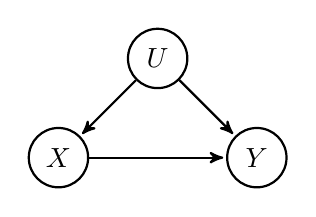
\begin{tikzpicture}[->,>=stealth',shorten >=1pt,auto,node distance=1cm,
  thick,main node/.style={punkt}]

 %nodes
\node[main node](1){$U$};
\node[main node, below left=of 1](2){$X$};
\node[main node, below right=of 1](3){$Y$};



 \path[every node/.style={font=\sffamily\small}]
    (1) edge node {} (2)
    	edge node {} (3)
    (2) edge node {} (3);
	
\end{tikzpicture} 
\end{subfigure}
\begin{subfigure}[t]{0.5\textwidth}
\centering
\caption{network after an intervention $G^*$}
\label{fig:mutilatedAfter}
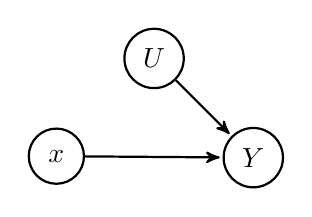
\begin{tikzpicture}[->,>=stealth',shorten >=1pt,auto,node distance=1cm,
  thick,main node/.style={punkt}]

 %nodes
\node[main node](1){$U$};
\node[main node, below left=of 1](2){$x$};
\node[main node, below right=of 1](3){$Y$};



 \path[every node/.style={font=\sffamily\small}]
    (1) edge node {} (3)
    (2) edge node {} (3);
    
\end{tikzpicture}
\end{subfigure}
\end{figure}


\begin{figure}[h]
\caption{}
\label{fig:causal_inference_without_do}
\centering
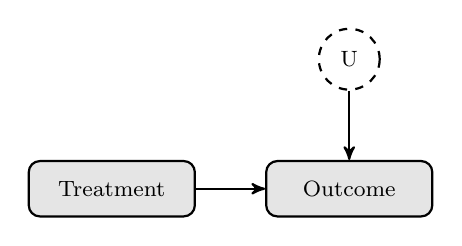
\begin{tikzpicture}[->,shorten >=0pt,shorten <=0pt,node distance=2.5em,thick,node/.style={observedrect},lt/.style={latent}]
\node[node](2){Treatment};
\node[node, right=of 2](3){Outcome};
\node[lt, above=of 3](4){U};
\path[]
	(2) edge (3)
	(4) edge (3);
	
\end{tikzpicture}
\end{figure}


There is a connection here to the degree to which the model is invariant. A model that is invariant to more things is more explanatory. We could look at levels of hierarchy. There is causal graphical models, which are invariant to interventions on variables. Can I tie this to a physical system and give more in depth examples of the nested tier of hierarchies?

I do not see the distinction between explanation and (causal) prediction. Explanation is all about the ability to compress and to generalise. The more a model can do this, the more we view as providing an understanding of the why. 


Sometimes the causal component is obvious. 

Relationship to generalisation. Variables causally directly causally related to the outcome (either causes or effects) should be more stable predictors over time. The assumption is there are less places for change to come in. 

If a feature is a cause of an outcome then changing the input distribution over that feature won't break the model. If its an effect it could.

The direct causes (and effects) of a variable of interest make up a sufficient set for prediction (is this true)? This may be a reason for using structure learning type algorithms even if you are simply doing prediction.

\subsubsection*{The role of assumptions in causal inference}

Fundamental challenges. How do you cross-validate or compare causal inference models? Lack of real world data on which to compare algorithms. 

Does predictive accuracy indicate a good causal model?

Assumptions must be recognised. Without assumptions - only description is possible. Recognising the assumption (and associated risk) means that we understand we should still attempt to experiment.

Generalising the results of one experiment to another (for example, dropping rocks to dropping people - with reference to the cross over trial for parachutes.) (This I think is the long term key to successful causal inference, learning from experimental data with representations that generalise). (and given sufficient generalisability, it may not matter if there is an underlying confounder - as this confounder is clearly not changing much)

Is causal inference possible (are the conclusions ever valid)?

Only from randomised experiment ... if people can do it without recourse to constant randomised experiment then an algorithm exits.

The challenges and limitations of inferring causal effects from observation data are numerous. However, there are problems we need to solve. The questions is are these problems so serious as to warrant disregarding all non-experimental data. I think answer is a clear no. Need ongoing validation, with assumptions. We can't validate the assumptions using the observational data alone (otherwise we would not have been forced to make them).


\subsection*{Relationship to interpretability}

A desire for interpretability indicates that something has been left out of the loss function. 

Are causal/interpretable models more reliable or more likely to generalise well? 

One form of interpretability gives people insight into what the features are that the model is relying on. 

If we know the training and test data will be sampled from different distributions, knowing what the features that the model is looking at are, allows people use their background understanding of the world to evaluate whether or not those features are likely to be transferable to the test domain. 

Specifically, people can
\begin{itemize}
\item rule out many possible features as highly unlikely to be relevant to a problem
\end{itemize}

People have access to a lot of detailed prior knowledge. 

\subsection*{Relationship to transfer learning}

find a feature representation in which $P(Y|X)$ is the same in many different domains (or stable over time). Causal models predict the outcome of actions. We could directly take these actions and learn $P(Y|a,X)$ for every $(a,X)$ but, in reality, no two situations (or actions) are exactly alike. So we have to make representations such that things are stable. 

This is tightly related to generalisability. If we take a person undergoing a medical test, we might describe the situation by the year and location, the person's age, gender, heart rate, medical condition and test results. We don't include , the color of the doctors shirt, the size of the room, ...

For example, in the advertising setting, we want to know how our on expenditure on paid search ads is linked to sales. However, this relationship may be very unstable over time because the ad slots are sold at auction. The amount we have to pay to obtain a given position for keyword depends crucially on the amount our competitors are bidding for that keyword. However, the relationship between displaying the ad at a particular position and the probability that someone clicks it an then makes a purchase may be much more consistent. 

Bandit feedback. The learner observes only the reward for the action they select. Not every possible option as in supervised learning.

\chapter{Introduction}

\paragraph*{My thesis in a sentence:} Unifying causal inference with multi-armed bandits.

\paragraph*{This thesis contributes to knowledge by:} Introducing a framework connecting causal graphical models with multi-armed bandits as a first step towards a unified approach to estimating the effect of interventions.  

\paragraph*{My key research questions are:} 
\begin{itemize}
\item To understand and the difference between prediction and causal inference in machine learning and clarify which problems require causal approaches.
\item To summarise the key strands of causal inference research from economics and social sciences for the machine learning community
\item To make connections between learning to act from observational versus experimental data. In particular, between causal graphical models and multi-armed bandits.
\end{itemize}



\section{Motivation}
Many of the most important questions in science and in our personal lives are about the outcomes of doing something. Will asking people to pay upfront at the doctors reduce long term health expenditure? If we developed a drug to suppress particular genes, could we cure MS and would delaying teen-aged pregnancies improve the outcome for their kids.  

These are hard questions because they require more than identifying a pattern in data. Correlation is not causation. Causal inference has proven so difficult that there is barely any consensus on even enduring questions like the returns to education or the long-term consequences of early life events – like teenage pregnancy, where the variables involved are susceptible to human intuition and understanding. 

We now live in a world of data. Hours of our lives are spent online, where every click can be recorded, tiny computers and sensors are cheap enough to incorporate into everything and the US Institute of Health is considering if all infants should be genetically sequenced at birth. Such data gives us a window into many aspects of our lives at an unprecedented scale and detail but it is messy, complicated and often generated as a by product of some other purpose. It does not come from the controlled world of a randomised experiment.

The rise of big data sets and powerful computers has seen an explosion in the application of machine learning. From healthcare, to entertainment and self driving cars; machine learning algorithms will transform many industries. It has been suggested that the impressive ability of statistical machine learning to detect complex patterns in huge data sets heralds the end of theory (Reference) and that we may be only a short step from the Singularity, where artificial intelligence exceeds our own and then grows exponentially. 

However, despite the huge advances in specific areas of machine learning (in particular deep learning), machine learning algorithms are effective only within very narrow problem settings. Getting them to generalise to even slightly different problems or data sets remains very challenging. Deciding how we should act or what policies we should implement requires us to be able to predict how a system will behave if we change it. The correlations detected by standard machine learning algorithms do not enable us to do this, no matter how many petabytes of data they are based on. As machine learning algorithms are incorporated into more and more of the decision making processes that shape the world we live it, it is critical to ensure that we understand the distinction between causality and prediction and that we develop techniques for learning how to act that are as effective as those we have for pattern recognition.


\section{What is causality and why do we care? (2000 words)}

The notion of causality has been widely debated in science and philosophy \cite{} but is still widely viewed as poorly defined \cite{}. This has led to a reluctance among applied researchers in many fields to refer to cauality in their work, leading them instead to report that variables are \textit{related}, \textit{correlated} or \textit{associated}. However, the magnitude, direction and even existance of an association depends on what other variables we adjust for (or include in a regression). Avoiding formalising causation, the real question of interest, leaves it up to the reader to determine via common sense if the association reported is the \emph{right one}. 

We discuss more detailed definitions of causality in section c


The what-if type questions from the why. \cite{Gelman2010} \cite{}. Why do whites to better than blacks in school (in America). Suggests that reverse causal inference questions are more interesting and motivate most of social science. 

I do not find this distinction useful. 
We can only change the future - history is useful only as far as it tells us something about the future.
Reverse causal questions can be reposed as forward ones, when making the translation a reverse causal query will be effectively asking about many possible interventions (rather than just one). Problems highlighted as intractible in the reverse causal sense are also intractible in the forward inference form, typically because concern situations for which we do not have a sufficient number of similar instances to allow statistical reasoning. For example, the war question posed in Gelman. 

A distinction between forward causal iference, what happens if we do X and reverse casual inference 

To explain or to predict \cite{Shmueli2010}
The two cultures \cite{Breiman2001}

\paragraph*{There are two reasons why correlation is not causation}. The first is related to variance and over-fitting. Observations are noisy. With a finite data set with enough variables we will be able to find some that are completely unrelated but correlate purely by chance. \ref{figure - search for random correlation}. The second arises from bias, typically introduced by an un-observed confounding variable. In this case, variables are correlated not by chance. We would expect the relationship to hold if we sampled more data. However, they are not causally related in that intervening to set one would not likely effect the other. EXAMPLE WITH FIGURE. 

\subsection{Defining causality}
\begin{itemize}
\item widely debated in science and philosophy (REFERENCES)
\item what is explanation?
\item any model that aims to predict the outcome of an action or intervention in a system
\item I do not see the distinction between explanation and (causal) prediction. Explanation is all about the ability to compress and to generalise. The more a model can do this, the more we view as providing an understanding of the why. 
\item mediation?
\end{itemize}
\subsection{Overview of this thesis}
\subsection{Identifying when we have a causal problem}

\subsubsection{Examples of typical machine learning problems. Are they causal?}

Consider the following problems, which span a wide range of the types of questions machine learning is currently being applied to. Which of them require casual inference? How can we identify characteristics of a problem that make causal modelling important?

\begin{itemize}
\item Speech recognition (for systems like Siri or Google)
\item Machine translation 
\item Image classification
\item Forecasting the weather
\item Playing Go 
\item Identifying spam emails
\item Automated essay marking
\item Predicting the risk of death in patients with pneumonia.
\item Predicting who will re-offend on release from prison 
\item Predicting which customers will cease to be your customers
\item Demand prediction for inventory control
\item Predicting who will click on an ad
\item Financial trading
\item Recommending movies
\item Online search
\item Self driving cars
\item Pricing insurance
\end{itemize}

The above problems are not posed with enough detail to know if causality is an important consideration. In particular, I failed to specify what actions the might be taken in response to model.

Consider speech recognition. You say something, which causes to sound waves, which are converted to a digital signal which Siri maps to words. Whatever action Siri takes is unlikely to change the distribution of words you use, and even less likely to change the function that maps sound waves to text (unless she sends you a DVD on elocution). A similar argument could be made for many applications of machine translation and image classification. 

In image recognition, we do not particularly care about building a strong model for exactly how the thing that was photographed translates to the image we see. We can be fairly confident that the process will not change. If we develop a discriminating model that is highly accurate at classifying cats from dogs, we do not care a lot about its internal workings (provided we have strong grounds to believe that the situations in which we will be using our model will match those under which it was trained).

What about forecasting the weather? If you are using a short term forecast to decide whether to pack an umbrella it's clear causality can be ignored - your decision will not effect if it actually rains. However, longer term climate forecasts might (theoretically) lead us to take action on emissions which would then change the weather system. For this we need a (causal) model that allows us to predict the outcome under various different interventions.

Identifying spam and automated essay marking systems are similar. The decision made by the algorithm is likely to change the relationship between the features used by the algorithm and the true label. Spammers and students will modify their writing in order to optimise their results. The standard machine learning approach can only work if the resulting change is sufficiently gradual and fresh ground truth (probably human labelled) training data is provided. (What would the nature of the features have to be such that change did not occur? - they would have to be causes of the label). 

What about predicting the risk of death in patients with pneumonia? Suppose we wish to use the model to decide who should be treated in hospital and who can be sent home with antibiotics. If we assume that in hospital treatment is more effective this seems like a straightforward prediction problem. It is not. Depending on how the decision to admit was previously made and what features are included (or omitted) in the model, the relationship between those features and the outcome may change if we start using the model to decide whom to admit. (xxx et al) found exactly this effect. Their model learnt that (among other things) people suffering asthma were \emph{less} likely to die from pneumonia. They realised this was because doctors were treating such patients very aggressively, thus actually lowering their risk. There is no problem with this model if you want to predict who would be likely to die whilst maintaining the original addmition and treatment protocols. However, using it to decide on what basis to admit people could kill. The key is understanding exactly what question you are asking. In this case we are care about what happens to patients with characteristics X if we treat them according to decision rule Z.   

Predicting which customers will leave or who will re-offend if granted parole also fit within the category of problems where you wish to identify a group for which a problem will occur and target some treatment to them (loyalty reward, deny parole or more support whilst on parole, etc). For all these problems the assumptions required to treat them as pure prediction problems are;
\begin{enumerate}
\item The treatment is assumed to be effective (at least better than nothing)
\item Deciding who to treat on the based of the model predictions won't change the relationship between features and outcome 
\end{enumerate}

Demand prediction seems relatively straightforward. These models use features such as location, pricing, marketing, time of year, weather, etc to forecast the demand for a product. It seems unlikely that using the model to ensure stock is available will itself change demand. However there is a potential data censoring issue. If demand is modelled by the number of sales, then if a product is out of stock demand will appear to be zero. Changing availability does then change demand.
   
Playing Go (and other games) is another case with some subtleties. At every turn, the AI agent has a number of actions available. The board state following each action is deterministic and given by the rules of the game. The agent can apply supervised machine learning based on millions of previous games to estimate the probability that each of these board states will lead to a win. ... this is interesting maybe come back to it ... an alternate approach would be to try to forecast the probability of a win given each action given the current board state as context ... One approach to causal inference is indeed to learn about actions from taking actions (or observing the actions that other have taken). When can we learn from the actions others have taken? When there is no confounding. And does this hold with Go? Probably because the board state encapsulates everything that should determine what move is played. Learning directly from actions and trying to generalise (can in some instances reduce the problem to standard ML)

Having considered these examples we can now identify some general aspects of the problem that determine whether or not we require a causal model.

\begin{itemize}
\item Does acting on the predictions of the model change the mapping from features to target? (at least if the decision process is open to scrutiny). In general, if we believe that humans are generally trying to optimise to various goals of their own then for any system interacting with them the answer to this will be yes.
\item 

 Covariate shift clearly comes in here. Because there are areas where mechanisms are understood it is relatively easy to argue that covariate shift is not occurring and that results will be transferable. The mechanism is known but the function may be complex. Can we write down something that causal models are invariant to in terms of shift that is not the case for non-causal models? Yes, if the way in which features get their values changes, then causal models will be invariant to that in a way that non-causal ones are not. 
 
\item To decide between actions we only need to rank them (not estimate their actual effect). 
\item The predicted outcome in the absence of an intervention provides a single point. We can use this to find which problems are most serious if left alone - and prioritise those for modelling changes. 
\item Any decision we take does not significantly impact the system from which the data was drawn to make it (for repeat decision making)
\item Does acting on the result of the prediction change the predictive distribution p(y|x)? Ie change people's behaviour.
\item Ethics - ... People's viewpoint on if its OK...
\end{itemize}

I hope these examples gave you a feel for the richness and subtitles of causal inference. We will return to some of them in more detail once we have established some more concrete language and tools to approach them with.



\section{Approaches to causality (1000 words)}

There are two broad approaches to deciding how to act. Reinforcement learning and causal inference. In reinforcement learning we estimate the effect of actions by taking them. We assume there is an agent capable of intervening in the system and try to find policies for the agent to follow in selecting actions so as to maximise some kind of reward. This is a very powerful and general framework (REFERENCES TO GENERAL AI). However, POINT OUT SOME OF THE DIFFICULTIES WITH REINFORCEMENT LEARNING. We are frequently presented with large bodies of data that have been collected from a system in which we did not have any control over what actions were taken. 

We will call data sets where we do not have control over the decision making process that generated the data observational. Versus experimental data sets, where we do have control (experimental data sets do not always have to be randomised -although that is a powerful approach to ensure we have control. There is a space in the middle where we have partially controlled the process by which agent select actions. Randomised data with imperfect compliance would be an example.


An agent (capable of intervening in the system) chooses an action from those available The agent making the decision included in the model. This is

Reinforcement learning addresses the problem of learning from explicitly taking actions. There
is typically some state or environment. An agent chooses an action from those available in the
current state. The state then evolves stochastically as a function of the selected action and
the agent receives some feedback or reward that is a function of the new state. This setting
differs from the standard classification problem in that the agent must learn from feedback on
the selected action, rather than being presented with the correct action for a given state. A
common modelling assumption is that the state evolves only as a function of the previous state
and the action chosen, and given these, is independent of the previous history of states and
actions. This is known as a Markov decision process or MDP. A particularly well studied and
understood model is the singe state MDP. In this case, there are a set of actions, each associated
with a fixed but unknown reward distribution and at each time step our agent selects an action
and receives corresponding feedback. This is known as the multi-armed bandit problem.

Causal inference makes use of assumptions to allow the outcome of actions to be predicted from
observational data. The key to causal inference is a framework that can model how actions
change the state of the world. This framework then allows us to map information collected in
one setting to another.

Both approaches can be seen as extensions to the concept of randomised controlled trials. Bandit
algorithms deal with the sequential nature of the decision making process, causal inference with
the problem that full randomisation is not always feasible, affordable or ethical. The similarities
between the problems that these techniques have been developed to address raises the question
of if there are problems best addressed by a combination of these approaches and how they
can be combined. The goal of my thesis is to explore these questions. In the next sections I
review the key literature in causal inference and bandits. I then present a general approach to
how causal models might be incorporated into bandit settings and conclude by demonstrating
an algorithm that leverages causal assumptions to improve performance in a specific bandit
setting.

There are two key approaches to causal problems. The first is to learn the outcome of actions by directly intervening in the system and seeing what happens. We then get feedback on how good those actions were. This is the approach taken in reinforcement learning. ADVANTAGES AND DISADVANTAGES OF THIS APPROACH. The second broad approach is causal inference. Here

\todo{insert figure showing data generating process and observed data defining ML}\ref{all of statistics}

\paragraph*{Two broad approaches} 
\begin{itemize}
\item Build a model to map the natural behaviour of the system to what will happen for some action
\item Take the action and see what happens
\end{itemize}

\paragraph*{The first is causal inference}

\paragraph*{The second is reinforcement learning}

\paragraph*{Both generalise from randomised experiment} Reinforcement learning to sequential decisions, causal inference to non-experimental conditions

Both these fields relate to the problem of making optimal decisions and both can be seen as generalising randomised controlled experiments. Causal inference  is the study of how to estimate the effect of an action in the absence of randomisation. Reinforcement learning studies how we can do better if the decisions are to be made sequentially. 

\paragraph*{Both approaches involve assumptions} the latter that we can group context and actions.

\paragraph*{Limitations of causal inference}

\paragraph*{Limitations of experiments} What are the issues with standard randomised experiments?



\chapter{Causal models}
\label{chap:causal_models}

Causal inference aims to infer the outcome of an intervention in some system from data obtained by observing (but not intervening in) it. To do this we need terminology to describe actions and how we anticipate the system should respond to them. Three key approaches have emerged; counterfactuals, structural equation models and causal bayesian networks. In this chapter we describe these approaches. We will examine what problems they allow us to solve, what assumptions they rely on and how they differ. We will also use them to describe the following simplified examples. The aim is to demonstrate the notations and formalisms we will need to tackle more interesting problems later on.

\vspace*{.3cm}
\begin{example}
\label{exm:ranomized_experiment}
Suppose we have developed a new drug for some illness and wish to determine how effective it is. We take a large group of patients and randomly assign half of them to a treatment group and the other half to a control group. The people in the treatment group get the drug, everyone else gets a placebo pill. The question we want to answer is does giving people the active drug improve their changes of recovery relative to giving them the placebo. We will use the variable $X$ (1 = drug, 0 = placebo) to represent the treatment each person receives and $Y$ (1 = recover, 0 = not recover) to describe the outcome. 
\end{example}

\vspace*{.3cm}
\begin{example}
\label{exm:adjusting}
Suppose we wish to estimate what would happen to high school graduation rates if we made pre-school available and compulsory for all 4 year olds. We have a large cross-secional dataset on a group of 20 year olds that records if they attended pre-school, if they graduated high school and their parents socio-economic status (SES). We will let $X\in \set{0,1}$ indicate if an individual attended pre-school, $Y \in \set{0,1}$ indicate if they graduated high school and $Z \in \set{0,1}$ represent if they are from a low or high SES background respectively.  
\end{example}


\section{Causal bayesian networks}

Causal Bayesian networks are an extension of Bayesian networks. A Bayesian network is a graphical way of representing how a distribution factorises. Any joint probability distribution can be factorised into a product of conditional probabilities. There are multiple valid factorisations, corresponding to permutations of variable ordering.

\eqn{
\label{eqn:cbn:joint_dist}
P(X_{1},X_{2},X_{3},...)=P(X_{1})P(X_{2}|X_{1})P(X_{3}|X_{1},X_{2})...
}

We can represent this graphically by drawing a network with a node for each variable and adding links from the variables on the right hand side to the variable on the left for each conditional probability distribution, see figure \ref{fig:bayesnet}. If the factorisation simplifies due to conditional independencies between variables, this is reflected by missing edges in the corresponding network. There are multiple valid Bayesian network representations for any probability distribution over more than one variable, see figure \ref{fig:bayesnet2} for an example. 

\begin{figure}[h]
\centering
\caption{A general Bayesian network for the joint distribution over three variables. This network does not encode any conditional independencies between its variables and can thus represent any distribution over three variables.}
\label{fig:bayesnet}
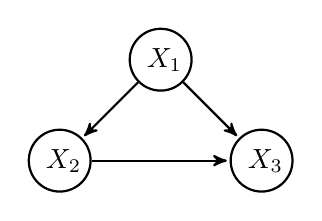
\begin{tikzpicture}[->,>=stealth',shorten >=1pt,auto,node distance=1cm,
  thick,main node/.style={punkt}]

 %nodes
\node[main node](1){$X_{1}$};
\node[main node, below left=of 1](2){$X_{2}$};
\node[main node, below right=of 1](3){$X_{3}$};


 \path[every node/.style={font=\sffamily\small}]
    (1) edge node {} (2)
    	edge node {} (3)
    (2) edge node {} (3);
	
\end{tikzpicture}
\end{figure}



\begin{figure}
\centering
\caption{Some valid Bayesian networks for a distribution that an be factorised as $\P{X_1,X_2,X_3} = \P{X_1}\P{X_2}\P{X_3|X_2}$ (which implies $X_3 \ci X_1 | X_2$)}
\label{fig:bayesnet2}
\begin{subfigure}[t]{0.15\textwidth}
\centering
\caption{}
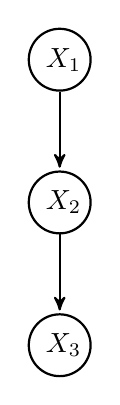
\begin{tikzpicture}[->,>=stealth',shorten >=1pt,auto,node distance=1cm, thick,main node/.style={punkt}]
 %nodes
\node[main node](1){$X_{1}$};
\node[main node, below=of 1](2){$X_{2}$};
\node[main node, below=of 2](3){$X_{3}$};
\path[every node/.style={font=\sffamily\small}]
    (1) edge (2)
    (2) edge (3);
\end{tikzpicture}
\end{subfigure}
\begin{subfigure}[t]{0.15\textwidth}
\centering
\caption{}
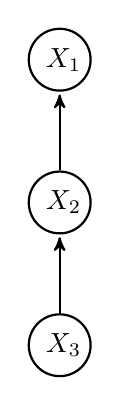
\begin{tikzpicture}[->,>=stealth',shorten >=1pt,auto,node distance=1cm, thick,main node/.style={punkt}]
 %nodes
\node[main node](1){$X_{1}$};
\node[main node, below=of 1](2){$X_{2}$};
\node[main node, below=of 2](3){$X_{3}$};
\path[every node/.style={font=\sffamily\small}]
    (3) edge (2)
    (2) edge (1);
\end{tikzpicture}
\end{subfigure}
\begin{subfigure}[t]{0.3\textwidth}
\centering
\caption{}
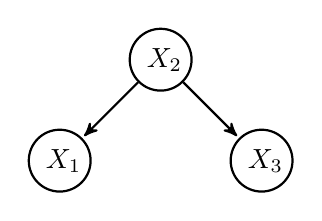
\begin{tikzpicture}[->,>=stealth',shorten >=1pt,auto,node distance=1cm, thick,main node/.style={punkt}]
 %nodes
\node[main node](1){$X_{2}$};
\node[main node, below left=of 1](2){$X_{1}$};
\node[main node, below right=of 1](3){$X_{3}$};
\path[every node/.style={font=\sffamily\small}]
    (1) edge (2) edge (3);
\end{tikzpicture}
\end{subfigure}
\begin{subfigure}[t]{0.3\textwidth}
\centering
\caption{}
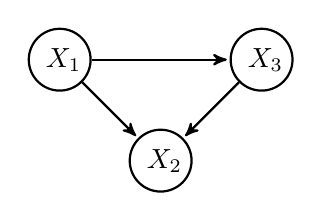
\begin{tikzpicture}[->,>=stealth',shorten >=1pt,auto,node distance=1cm, thick,main node/.style={punkt}]
 %nodes
\node[main node](1){$X_{2}$};
\node[main node, above left=of 1](2){$X_{1}$};
\node[main node, above right=of 1](3){$X_{3}$};
\path[every node/.style={font=\sffamily\small}]
    (2) edge (1)
    (3) edge (1)
    (2) edge (3);
\end{tikzpicture}
\end{subfigure}
\end{figure}



The statement that a given graph $G$ is a Bayesian network for a distribution $P$ tells us that the distribution can be factorised over the nodes and edges in the graph. There can be no missing edges in $G$ that do not correspond to conditional independencies in $P$ (the converse is not true $G$ can have extra edges). If we let $parents_{X_{i}}$ represent the set of variables that are parents of the variable $X_{i}$ in $G$ then we can write the joint distribution as; 

\begin{equation}
P(X_{1}...X_{N}) = \prod_{i = 1...N}P(X_{i}|parents_{X_{i}})
\end{equation}

A causal Bayesian network is a Bayesian network in which it a link $X_{i} \rightarrow X_{j}$, by definition, implies $X_{i}$ causes $X_{j}$. This means that if we intervene and change the value of $X_{i}$, we expect $X_{j}$ to change, but if we intervene to change $X_{j}$, $X_{i}$ will not change. We need some notation to describe interventions and represent distributions over variables in the network after an intervention. In this thesis I use the do operator introduced by Pearl \citep{Pearl2000}.


\begin{definition}{The do-notation}
\begin{itemize}
\item do(X=x) denotes an intervention that sets the random variable(s) $X$ to $x$.
\item $\P{Y|do(X)}$ is the distribution of $Y$ conditional on an \emph{intervention} that sets $X$. This notation is somewhat overloaded. It may be used represent a probability, a probability distribution/mass function or a family of distribution functions depending on if the variables are discrete or continuous and whether or not we are treating them as fixed. For example it could represent 
\begin{itemize}
\item The probability $\P{Y=1|do(X=x)}$ as a function of $x$
\item The probability mass function for a discrete $Y$ : $\P{Y|do(X=x)}$
\item The probability density function for a continuous  $Y$ : $f_Y(y|do(X=x))$
\item a familiarly of density/mass function for $Y$ paramaterised by $x$.
\end{itemize}
Where the distinction is important not clear from context we will use one of the more specific forms above. 
\end{itemize}
\end{definition}


\begin{theorem}[Truncated product formula]
\label{thm:truncated_prodcut}
If $G$ is a causal network for a distribution $P$ defined over variables $X_{1}...X_{N}$, then we can calculate the distribution after an intervention where we set $Z \subset X$ to $z$, denoted $do(Z=z)$ by simply dropping the terms for each of the variables in $Z$ from the factorisation given by the network \citep{Pearl2000}. 

\begin{equation}
\label{eq:truncatedproduct}
\P{X_1...X_N|do(Z=z)} =
  \begin{cases}
  \prod_{i \notin Z}\P{X_{i}|parents_{X_{i}}} & \text{if $(X_{1}...X_{N})$ consistant with $Z=z$}  \\
   0       & \text{otherwise } 
  \end{cases}
\end{equation}
\end{theorem}


Theorem \ref{thm:truncated_prodcut} does not hold for standard bayesian networks for the simple reason that there are multiple valid networks for the same distribution. The truncated product formula will give different results depending on which you choose. The result is possible with causal bayesian networks because it follows directly from the assumption that the direction of the link indicates causality. In fact, from the interventionist viewpoint of causality, the truncation product formula defines what it means for a link to be causal. 


Returning to example \ref{exm:ranomized_experiment}, and phrasing our query in terms of interventions; what would the distribution of outcomes look like if everyone was treated $\P{Y|do(X=1)}$, relative to if no one was treated $\P{Y|do(X=0)}$? The treatment $X$ is a potential cause of $Y$, along with other unobserved variables, such as the age, gender and disease sub type of the patient. Since $X$ is assigned  via deliberate randomisation we know that it is not effected by any latent variables. The causal bayesian network for this scenario is shown in figure \ref{fig:causal_network_example} .This network represents the (causal) factorisation  $\P{X,Y} = \P{X}\P{Y|X}$, so from equation (\ref{eq:truncatedproduct}), $\P{Y|do(X)} = \P{Y|X}$. In this example, the interventional distribution is equivalent to the observational one.

\begin{figure}[h]
\caption{Causal Bayesian network for example \ref{exm:ranomized_experiment}}
\label{fig:causal_network_example}
\centering
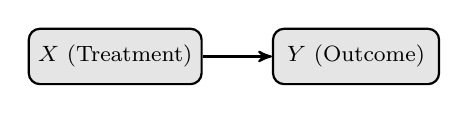
\begin{tikzpicture}[->,shorten >=0pt,shorten <=0pt,node distance=2.5em,thick,node/.style={observedrect},lt/.style={latent}]
\node[node](2){$X \text{ (Treatment)}$};
\node[node, right=of 2](3){$Y \text{ (Outcome)}$};
\path[]
	(2) edge (3);
\end{tikzpicture}
\end{figure}



In example \ref{exm:adjusting} we are interested $\P{Y|do(X=1)}$, the expected high-school graduation rate if we introduce universal preschool. We could compare it to outlawing pre-school $\P{Y|do(X=0)}$ or the current status quo $\P{Y}$. It seems reasonalble to assume that attending could pre-school effect the likelyhood of graduating from high school and that your parents socio-economic status effects both pre-school attendance and high-school graduation. If we assume that socio-economic status is the only such variable (nothing else effects both attendance \emph{and} graduation), we can represent this problem with the causal bayesian network in figure \ref{exm:adjusting}. In this case, the interventional distribution is not equivelent to the observational one. If better off parents are more likely to send their children to pre-school these children more likely to graduate high school regardless, then simply comparing the high school graduation rates of those who attended preschool with those who did not will overstate the benifit of preschool. To obtain the interventional distribution we have to estimate the benifit of preschool for each socio-economic level seperately and then weight the results by the proportion of the population in that group, $\P{Y|do(X=1)} = \sum_{z \in Z}\P{Y|X=1,Z}\P{Z}$. 

We have seen from these two examples that the expression to estimate the causal effect of an intervention depends on the structure of the causal graph. There is a very powerful and general set of rules that specify how we can transform observational distributions into intervetional ones for a given graph structure. These rules are referred to as the Do-calculus \cite{Pearl2000}. We discuss them further in section \ref{}. 


\begin{figure}
\center
\caption{Causal bayesian network for example \ref{exm:adjusting}}
\label{fig:causal_adjust}
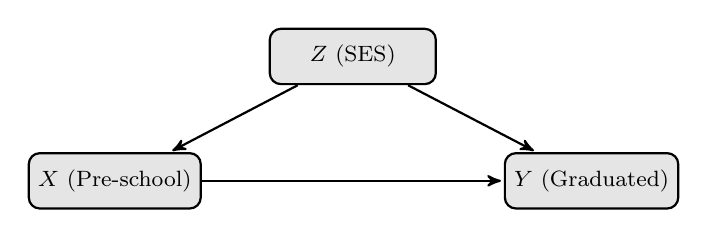
\begin{tikzpicture}[->,>=stealth',shorten >=1pt,auto,node distance=1.2cm, thick,node/.style={observedrect},lt/.style={latent}]

 %nodes
\node[node](1){$Z \text{ (SES)}$};
\node[node, below left=of 1](2){$X \text{ (Pre-school)}$};
\node[node, below right=of 1](3){$Y \text{ (Graduated)}$};
\path[every node/.style={font=\sffamily\small}]
    (1) edge (2) edge (3)
    (2) edge (3); 
\end{tikzpicture} 
\end{figure}

Formalising the definition of an intervention within the framework of causal graphical models provides us with an explicit mechanism to map information from one data generating process, the system pre-intervention, to another, the system post-intervention. The power of defining an intervention in this way stems from the number of things that are invariant between the two processes. All the (conditional) distriubtions for variables in the graph that were not directly set by the intervention are assumed not be changed by it.  

We could represent problems of the type where we try to infer properties of the post-interventional system based on data generated by the pre-interventional distribution by explicitly representing both systems and what they have in common, see figure \ref{fig:causal_ordinary_bayes}. This does not require any special framework or notation. The graphs in figure  \ref{fig:causal_ordinary_bayes} are ordinary Bayesian networks. However, without a causal framework, we have to make assumptions about what will be invarient to the intervention specifically for each such problem we encounter. For complex problems, it is very difficult to conceptualise what assumptions we expect to hold without the benifit of a causal framework.  


\begin{figure}[h]
\center
\caption{Causal inference with ordinary bayesian networks. The plate on the left represents the observed data generated prior to the intervention and the plate on the right the data we anticipate obtaining after an intervention that the pre-interventional variable $X$ to $x$. The assumptions characterised by this plate model correspond to those implied by the causal bayesian network in figure \ref{fig:causal_adjust} for the intervention $do(X=x)$. As the networks in this figure are ordinary Bayesian networks, we could have represented the same information with a different ordering of the links within each plate. However, we would then have a complex transformation relating the parameters between the two plates rather than a simple invariance.}
\label{fig:causal_ordinary_bayes}
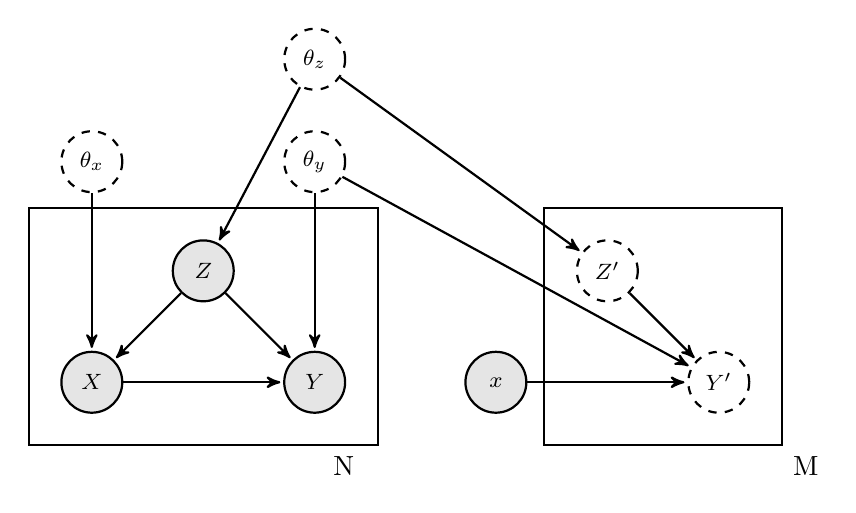
\begin{tikzpicture}[->,>=stealth',shorten >=1pt,auto,node distance=1.2cm, thick,node/.style={observed},lt/.style={latent}]
\tikzstyle{box}=[rectangle, draw=black!100]
 %nodes
\node[node](1){$Z$};
\node[node, below left=of 1](2){$X$};
\node[node, below right=of 1](3){$Y$};
\node[node, right=1.5cm of 3](4){$x$};
\node[lt, above right=of 4](5){$Z'$};
\node[lt, below right=of 5](6){$Y'$};
\node[lt, above=2.0cm of 3](9){$\theta_{y}$};
\node[lt, above=0.5cm of 9](7){$\theta_z$};
\node[lt, above=2.0cm of 2](8){$\theta_x$};
\path[every node/.style={font=\sffamily\small}]
    (1) edge (2) edge (3)
    (2) edge (3)
    (4) edge (6)
    (5) edge (6)
    (8) edge (2)
    (7) edge (1) edge (5)
    (9) edge (3) edge (6);
\node[rectangle, inner sep=4.0mm, fit= (1) (2) (3),draw=black!100,label=below right:N] {};
\node[rectangle, inner sep=4.0mm, fit= (5) (6),draw=black!100,label=below right:M] {};
\end{tikzpicture} 
\end{figure}

A causal bayesian network represents much more information than a bayesian network with identical structure. A causal network encodes all possible interventions that could be specified with the do-notation. For example, if the network in figure \ref{fig:causal_adjust} were an ordinary bayesian network and all the variables were binary, the associated distribution could be described by 7 parameters. The equivelent causal bayesian network additionally represents the post-interventional distributions for six possible single variable interventions and twelve possible two variable interventions. Encoding all this information without the assumptions implicit in the causal bayesian network would require and additional 30 parameters. \footnote{After each single variable intervetion we have a distribution over two variables, which can be represented by three parameters. After each two variable intervention, we have a distribution over one variables which requires one parameter. This takes us to a total of $6*3+12*1 = 30$ additional parameters.}


Causal bayesian networks are bayesian networks so results that apply to bayesian networks carry directly across;the local Markov property states that variables are independent of their non-effects given their direct causes. Similarly the global Markov property and d-separation also hold in causal networks. 

\subsubsection{Limitations of causal bayesian networks}
A number of criticisms have been levelled at this approach to modelling causality. One is that the definition of an intervention only in terms of setting the value of one or more variables is too precise and that any real world intervention will effect many variables in complex and non-deterministic ways \citep{2009causality,cartwright2007hunting}. However, the deterministic $do()$ operator turns out to be surprisingly effective at modelling more complex interventions by augmenting the causal graph with additional variables that model how our interventions may take effect. For example, in our drug treatment case we assumed we set the drug that each person receives. But what if some people in fact fail to take the prescribed treatment? How can we model this within the framework of deterministic interventions? We add a node representing what we prescribed to them (which we intervene on), which probabilistically influences what treatment they actually receive. See figure \ref{fig:randomized_imperfect_compliance}. Note that the fact that we no longer directly assign the treatment opens the possibility that an unobserved latent variable could effect both the actual treatment taken and the outcome.

The causal effect may provide useful bounds on the actual quantity of interest. 

\begin{figure}[h]
\caption{Randomised treatment with imperfect compliance}
\label{fig:randomized_imperfect_compliance}
\centering
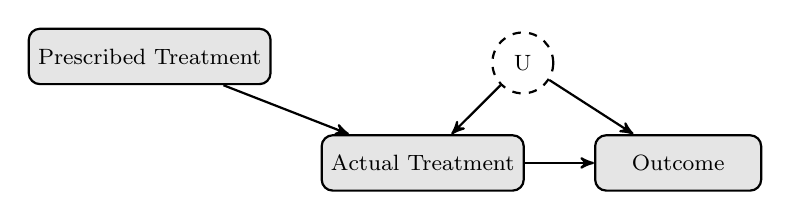
\begin{tikzpicture}[->,shorten >=0pt,shorten <=0pt,node distance=2.5em,thick,node/.style={observedrect},lt/.style={latent}]
\node[node](1){Prescribed Treatment};
\node[node, below right=of 1](2){Actual Treatment};
\node[node, right=of 2](3){Outcome};
\node[lt, above left=of 3](4){U};
\path[]
	(1) edge (2)
	(2) edge (3) 
	(4) edge (3) edge (2);
\end{tikzpicture}
\end{figure}

Another key issue with causal bayesian networks is that they cannot handle cyclic dependencies between variables. Such feedback loops are common in real systems, for example the relationship between supply and demand in economics or preditor and prey in ecology. We might regard the underlying causal mechanisms in these examples to be acyclic; the number of preditors at one point in time influences the number of prey in the next and so on. However, if our measurements of these variables must be aggregated over timeframes that are longer than the scale at which these interactions occure the result is a cyclic dependency. Even were we able to measure on shorter timescales, we might then not have sufficient data on each variable for inference. Such problems have mostly been studied within the dynamic systems liturature, typically focusing on understanding the stationary or equilibrium state of the system and making very specific assumptions about functional form in order to make problems tractable. \citep{Poole2013} compare the equilibrium approach to reasoning about cyclic problems with strucural equation models, which we discuss in section \ref{sec:SEM} and which can be seen as bayesian causal networks with additional functional assumptions. 

\section{Counterfactuals}

The Neyman-Rubin model \cite{Rubin1974,Rubin1978,Rosenbaum1983, Rubin2005,Rubin2008} defines causality in terms of potential outcomes, or counterfactuals. Counterfactuals are statements about imagined or alternate realities, are prevalent in everyday language and may play a role in the development of causal reasoning in humans \cite{Weisberg2013}. Causal effects are differences in counterfactual variables; what is the difference between what would happen if we did one thing versus what would happen if we did something else. 

In our example, the causal effect of the drug relative to placebo for person $i$ is the difference between what would happen if they were given the drug, denoted $y_{i}^{1}$ versus what would happen if they got the placebo, $y_{i}^{0}$. The fundamental problem of causal inference is that we can only observe one of these two outcomes, since a given person can only be treated or not treated. The problem can be resolved if, instead of people, you have units you can assume are identical or that will revert exactly to their initial state some time after treatment. This type of assumption often holds to a good approximation in the natural sciences and explains why researchers in these fields are less concerned with causal theory. 

Instead of trying to estimate individual effects, lets see if we can learn something about the distributions under treatment or placebo.  Let $\cf{Y}{1}$ be a random variable representing the potential outcome if treated. The distribution of $\cf{Y}{1}$ is the distribution we would see of $Y$ if everyone was treated. Similarly $Y^{0}$ represents the potential outcome for the placebo. We want to know the difference between the probability of recovery, across the population if everyone was treated, and the probability of recovery given placebo  $\P{\cf{Y}{1}}-\P{\cf{Y}{0}}$. We can estimate, from an experimental or observational study, the probability that people recover if treated $P(Y|X=1)$ and the probability that they recover if not treated $P(Y|X=0)$. Now if $X=0$ then $Y = \cf{Y}{0}$. Equivalently stated:

\eq{
\P{Y^{0}|X=0}&= \P{Y|X=0}\\
\P{Y^{1}|X=1}&=P{Y|X=1}
}

If we assume $X \ci Y^{0}$ and $X \ci Y^{1}$:

\eq{
\P{Y^{1}} &= \P{Y^{1}|X=1} = \P{Y|X=1} \\
\P{Y^{0}} &= \P{Y^{0}|X=0} = \P{Y|X=0}
}

\eq{
\implies \P{Y^{1}}-\P{Y^{0}} = \P{Y|X=1} - \P{Y|X=0}
}

The assumptions $X \ci Y^{1}$ and $X \ci Y^{0}$  are referred to as ignore-ability assumptions \cite{Rosenbaum1983}. They state that the treatment a each person receives is independent of whether they would recover if treated and if they would recover if not treated. Again this is justified in our example due to the randomisation of treatment assignment. In general these assumption do not hold. If people were deciding whether or not to buy the treatment, rather than it being randomly assigned, there could be a variable, for example income,D-separation still applies in the augmented model. that influenced both the decision to get treatment and the likelihood of recovery given treatment or placebo.

\todo{SUTVA assumption}

There are some complex philosophical objections to counter factuals arising from the way they describe alternate universes that were never realised and are not empirically testable \ref{XXXXX}. This can result in some concrete problems. Consider the following example based on  \ref{Dawid2000}.

Again we have a drug, where the outcome for an individual if treated is represented by the counterfactual variable $\cf{Y}{1}$ and the outcome if not treated is $\cf{Y}{0}$. Suppose these counterfactual variables $\cf{Y}{1}$ and $\cf{Y}{0}$ are jointly normal. We will assume equal variance for simplicity.

% vector with mean mu_t,mu_c and a covariance matrix
\eq{
P(Y_t,Y_c) \sim N()
}

then their difference is also normal,

\eq{
P(\tau) = N(\mu_t - \mu_c,2\sigma^{2}(1-\rho))
}

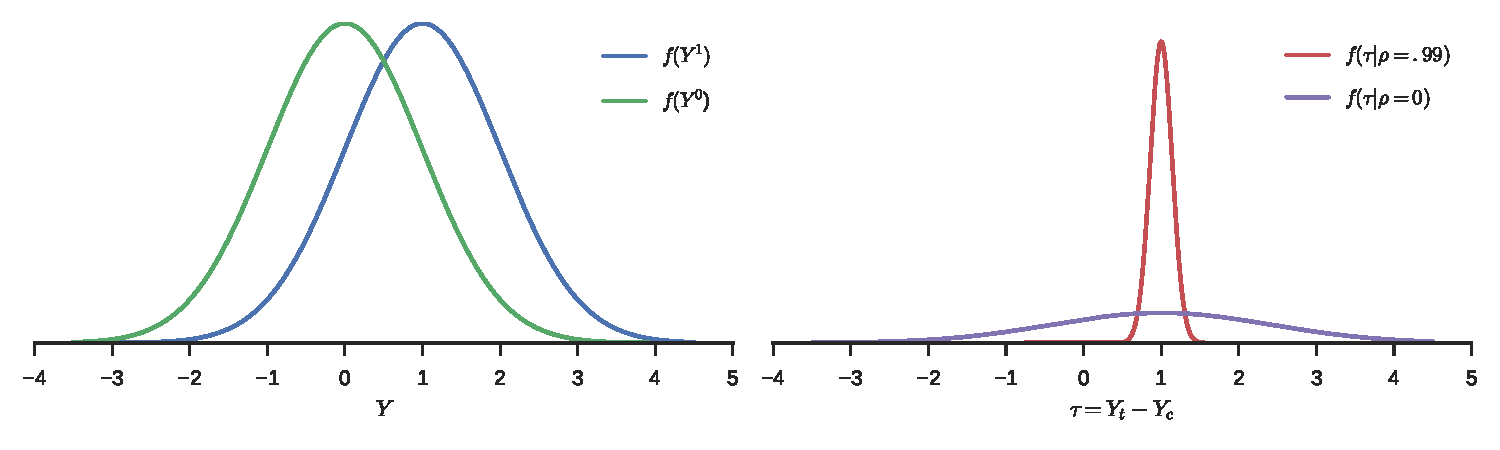
\includegraphics[scale=.6]{figures/counterfactual_nonidentify.pdf}

Key issue is that we can never observe the joint distribution over $Y_t$ and $Y_c$. As a result, the variance of $\tau$ is not identifiable, even from experimental data. It seems on the face of it that $\tau$ is relevant to our decision making. If the example above, if $\rho = 1$ then almost everyone benefits slightly from the treatment. However if $\rho=0$, there is a wide range, with some people benefiting a lot and others suffering significant harm.  

Can these issues be resolved? If so, how? 

- note that we can bound this counterfactual distribution based on the variance of the observed interventional distributions. If the variance of XXX is small then this may not be an issue. 

- does it actually make sense to make a decision on the basis of this counterfactual that is a function of something we could never observe. I

- part of the problem may be due to the deterministic way we have phrased individual treatment effects. 

Can these issues be resolved by considering personalised causal effects as random variables and avoiding counterfactuals?

A range of similar issues can arise in counterfactuals \ref{XXXX}. 
- What assumptions are required for the kind of counterfactual analysis like X would have been higher had B ...?
- briefly discuss the different flavours of counterfactual questions here. 

One way of looking at counterfactuals is as a natural language short hand for describing highly specific interventions like those denoted by the do-notation. Rather than taking about the distribution of Y given we intervene to set $X=x$ and hold everything else about the system constant we just say what would the distribution of $Y$ be had $X$ been $X$. This is certainly convenient, if rather impressive. 

\section{Structural Equation models}
\label{sec:SEM}

Structural equation models (SEMs) describe a deterministic world, where some underlying mechanism or function determines the output of any process for a given input. The mechanism (but not the output) is assumed to be independent of what is fed into it. Uncertainties are not inherent but arise from unmeasured variables. Linear structural equation models have a long history for causal estimation \cite {Wright1921,Haavelmo1943}. More recently, they have been formalised, generalised to the non-linear setting and connected to developments in graphical models to provide a powerful causal framework \cite{Pearl2000}.

Mathematically, each variable is a deterministic function of its direct causes and a noise term that captures unmeasured variables. The noise terms are required to be mutually independent. If there is the possibility that an unmeasured variable influences more than one variable of interest in a study, it must be modelled explicitly as a latent (unobserved) variable. Structural equation models can be represented visually as a network. Each variable is a node and arrows are drawn from causes to their effects. For example \ref{exm:ranomized_experiment} the SEM is:


\begin{figure}[h]
\caption{SEM for examples \ref{exm:ranomized_experiment}}
\label{fig:causal_network_example2}
\centering
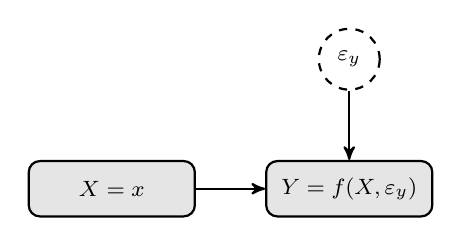
\begin{tikzpicture}[->,shorten >=0pt,shorten <=0pt,node distance=2.5em,thick,node/.style={observedrect},lt/.style={latent}]
\node[node](2){$X = x$};
\node[node, right=of 2](3){$Y = f(X,\epsilon_y)$};
\node[lt, above=of 3](4){$\epsilon_y$};
\path[]
	(2) edge (3)
	(4) edge (3);
\end{tikzpicture}
\end{figure}

This model encodes the assumption that the outcome $y_{i}$ for an individual $i$ is caused solely by the treatment $x_{i}$ they receive and other factors $\epsilon_{y_{i}}$ that are independent of $X$. This is justifiable on the grounds that $X$ is random. The outcome of a coin flip for each patient should not be related to any of their characteristics (hidden or otherwise). Note that the causal graph in figure \ref{fig:causal_network_example2} is identical to that the bayesian network for the same problem, figure \ref{fig:causal_network_example}. The latent variable $\epsilon_y$ was not explicitly drawn in figure \ref{fig:causal_network_example} as the noise can be captured within the probabilistic node, however adding it would not change the model. 
 

We want to estimate the causal effect of treatment; what is the probability of recovery if we \textbf{take the action} 'treat' versus the \textbf{action} 'placebo'? Taking the action 'treat'  corresponds to replacing the equation $X = \epsilon_{x}$ with $X=1$. The probability distribution over $Y$ given we set $X=1$ is then $P(Y = y|do(X=1)) = P(f(1,\epsilon_{y})=y)$, where we have introduced the $do$ notation to distinguish setting a variable from observing it \cite{Pearl1995}. However, for this model,  The probability of observing $Y$ given $X=1$, $P(Y = y|X = 1)$ is also given by $P(f(1,\epsilon_{y})=y)$ because $\epsilon_{y} \ci \epsilon{x}$. The causal effect is exactly the difference in observed outcomes, as we would intuitively expect for a randomised experiment. In this case, due to the assumption that $X \rightarrow Y$ and that there is no hidden common cause, correlation is causation.  

For a model with $N$ variables, a structural equation model looks like a set of $N$ simultaneous equations, with each variable playing the role of the dependent (left hand side) variable in one equation. However a SEM is, by definition, more than a set of simultaneous equations. By declaring it to be structural we are saying that it represents assumptions about the relationships between variables. When we visualise the model as a network the absence of an arrow between two variables encodes the assumption that one does not cause the other.


Limitations \& Criticisms 
- can express some non-measurable things
	- example of that

- confusion may occur as to whether interpretation is causal

- can they handle cycles?





\section{Comparing and unifying the models}

Remarkably for models developed relatively independently in fields with very different approaches and problems, the models we have discussed can be nicely unified for interventional queries (those that can be expressed with the do-notation). This makes it straightforward to combine key results and algorithms developed within any of these frameworks. For example, draw a graphical network to determine if a problem is identifiable and which variables should be adjusted for to obtain an unbiased causal estimate. Then use propensity scores \ref{} estimate the effect. If non-parametric assumptions are insufficient for identification or lead to overly large uncertainties, you can specify additional assumptions by phrasing your model in terms of structural equations. 

If the network for a structural equation model is acyclic, that is if starting from any node and following edges in the direction of the arrows you cannot return to the starting point, then it implies a recursive factorisation of the joint distribution over its variables. In other words, the network is a causal Bayesian network. All of the results that apply to causal Bayesian networks also apply to acyclic structural equation models.  Taking an action that sets a variable to a specific value equates to replacing the equation for that variable with a constant. This corresponds to dropping a term in the factorisation and the truncated product formula (equation \ref{eq:truncatedproduct}). Thus, the interventional query $P(Y|do(X))$ is identical in these two frameworks. We can also connect this to counterfactuals via:

\begin{equation}
\begin{aligned}
&Y^{0} \equiv P(Y|do(X=0)) \\
&Y^{1} \equiv P(Y|do(X=1))
\end{aligned}
\end{equation}

The assumption $\epsilon_{X} \ci \epsilon_{Y}$, stated for our structural equation model, translates to $X \ci (Y^{0},Y^{1})$ in the language of counterfactuals. When discussing the counterfactual model, we actually made the slightly weaker assumption:

\begin{equation}
\label{eq:weakignore}
X \ci Y^{0} \text{ and } X \ci Y^{1}
\end{equation}

It is possible to relax the independence of errors assumption we made for SEMs slightly to correspond exactly the form of equation (\ref{eq:weakignore}) without losing any of the power provided by d-separation and graphical identification rules \cite{Richardson2013}. To determine if and how an interventional query can be non-parametrically identified, it is equivalent to specify assumptions graphically in terms of functional models or bayesian networks or as conditional independence statements involving counterfactual variables (ignorability assumptions). By non-parametrically, I mean that we are not making any assumptions about the form of the relationships between variables. Models that are not non-parametrically identifiable can still be identified given assumptions about the distributions of variables and the functional relationship between them, for example, that the functions are linear or that the noise is additive \cite{Peters2014}. This form of assumption fits extremely naturally into the structural equation framework. 


However we can also pose causal queries that are not interventional and cannot be phrased in terms of the do-notation. The patients in our drug treatment example could be broken down into four groups. \todo{point out objections to doing this}. The first group will recover whether or not they receive treatment, the second group will recover if treated but not on the placebo, the third group will recover on the placebo and not if treated, and the last group will not recover on treatment or placebo. Unfortunately, we don't know which group each person belongs to. Drawing this up as a table:

\begin{tabular}{c|c|c|c}
group & placebo & treatment & probability of group\\
\hline
1 & die & die & $\alpha=P(Y^{0}=0,Y^{1}=0)$\\
2 & die & recover & $\beta=P(Y^{0}=0,Y^{1}=1)$\\
3 & recover & die & $\gamma=P(Y^{0}=1,Y^{1}=0)$\\
4 & recover & recover & $\delta=P(Y^{0}=1,Y^{1}=1)$\\
\end{tabular}

The queries we have been asking thus far are about $P(Y^{0}=1) = \gamma + \delta$ and $P(Y^{1}=1) = \beta + \delta$, but suppose we asked the question; what is the probability that this patient, who was not treated and died, would have recovered if they had been treated? We know they are in either group 1 or 2 since they died without treatment, so the answer is $\frac{\beta}{\alpha+\beta}$. Can we estimate the $\alpha, \beta, \gamma, \delta$ or in other words, identify the joint distribution over the counterfactuals $P(Y^{0},Y^{1})$ given the interventional distributions, $P(Y^{0})$ and $P(Y^{1})$? The answer is no, putting our constraints and unknowns in matrix form:

\begin{equation}
\left(
\begin{array}{cccc}
0&0&1&1\\
1&1&0&0\\
0&1&0&1\\
1&0&1&0\\
1&1&1&1\\
\end{array}
\right)
\left(
\begin{array}{c}
\alpha\\
\beta\\
\gamma\\
\delta\\
\end{array}
\right)= 
\left(
\begin{array}{c}
P(Y^{0})\\
1-P(Y^{0})\\
P(Y^{1})\\
1-P(Y^{1})\\
1\\
\end{array}
\right)
\implies
\left(
\begin{array}{c}
\alpha\\
\beta\\
\gamma\\
\delta\\
\end{array}
\right)=
\left(
\begin{array}{c}
1-P(Y^{0})-P(Y^{1})+\delta\\
P(Y^{1})-\delta\\
P(Y^{0})-\delta\\
\delta\\
\end{array}
\right)
\end{equation}
The value of $\delta$ is not determined so the query is not identifiable. However we do get bounds on the terms. Since probabilities cannot be negative, $P(Y{1})-P(Y^{0})-1 \leq \delta \leq min(P(Y^{1}),P(Y^{0})$. Note, if we made the additional assumption $\gamma=0$; that the drug did not cause anyone to die who would otherwise have survived, then we can determine the joint distribution over counterfactuals. Alternatively, if we could assume that after treatment people returned to their initial state after some period of time, (say we were testing a drug for acne) then we could run a crossover study to determine the joint distribution. In a crossover study, the participants are randomly assigned to treatment and placebo, results are measured and then the groups are swapped. The scientific and philosophical validity of counterfactual queries remains under question \cite{Dawid2000,Dawid2014}, however they are nonetheless widely posed in the form of attribution of causal effects to different pathways and mediation \cite{Pearl2014,Imai2010a,VanderWeele2011}. 

There are differences between the models we have considered when it comes to counterfactual queries. Counterfactuals are not defined in causal Bayesian networks, as they only encode information on the interventional distribution over variables.  Counterfactuals can be defined in terms of structural equation models \cite{Pearl2000} but there are subtle differences depending on the form of assumptions made. Structural equation models with independent errors allows the identification of quantities in mediation studies, which are not identifiable with the weak ignorability assumptions and cannot be tested experimentally \cite{Richardson2013}.  

In practice, differences in focus and approach across different fields eclipse these actual differences in the models. The work on causal graphical models \cite{Pearl2000,Sprites} focuses on non-parametric estimation in the population limit and rigorous theoretical foundations. The Neyman-Rubin framework builds on our understanding of randomised experiment and generalises to quasi-experimental and observational settings, with a particular focus on non-random assignment to treatment. This research emphasises estimating average causal effects and provides practical methods for estimation, in particular, propensity scores; a method to control for multiple variables in high dimensional settings with finite data \cite{Rosenbaum1983}. In economics, inferring causal effects from non-experimental data so as to support policy decisions is central to the field. Economists are often interested in broader measures of the distribution of causal effects than the mean and make extensive use of structural equation models, generally with strong parametric assumptions \cite{Heckman2008}. In addition, the parametric structural equation models favoured in economics can be extended to analyse cyclic (otherwise referred to as non-recursive) models. 


\subsubsection{A translator from graphical independence to counter factual statements}

\subsubsection{More terminology}
With the graphical framework in place, it is useful to define some key terminology used in describing causal models in terms of the graph structure they refer to.

\begin{enumerate}
\item confounding
\item exogenous
\item endogenous
\item nuisance variables
\end{enumerate} 

\section{What does a causal model give us? Resolving Simpson's paradox}

We will now demonstrate how we can use our new notation and frameworks for causal inference to resolve a fascinating paradox.  \todo{ insert some history of Simpson's paradox here.}

\cite{simpson1951interpretation}

Suppose a doctor has two treatments, A and B, which she offers to patients to prevent heart disease. She keeps track of which medication her patients choose and whether or not the treatment is successful. She obtains the results in table \ref{tab:simpson1}.

\begin{table}[h]
\label{tab:simpson1}
\caption{Treatment results}
\center
\begin{tabular}{c c c c c}
Treatment & Success & Fail & Total & Success Rate\\
\hline
\rowcolor[gray]{0.9} 
A &  87 & 13 & 100 & 87\%\\
\rowcolor{white} B & 75 & 25 & 100 & 75\%\\
\hline
\end{tabular}
\end{table}

It looks like drug A is performing better. However, having read the latest literature on how medications effect men and women differently, she decides to break down her results by gender to see how well the drugs perform for each group and obtains the data in table \ref{tab:simpson2}.

\begin{table}[h]
\label{tab:simpson2}
\caption{Treatment results by gender}
\center
\begin{tabular}{c c c c c c}
Gender & Treatment & Success & Fail & Total & Success Rate\\
\hline
\rowcolor[gray]{0.9}
M & A & 12 & 8 & 20 & 60\%\\
M & B & 56 & 24 & 80 & 70\%\\
\rowcolor[gray]{0.9}
F & A & 75 & 5 & 80 & 94\%\\
F & B & 19 & 1 & 20 & 95\%\\
\hline
\end{tabular}
\end{table}

Much to her surprise, once the data is broken down by gender, Treatment B looks better for both men \emph{and} women. Suppose the doctor must choose only one drug to prescribe to all her patients in future (perhaps she must reccomend which to subsidise under a national health scheme). Should she choose A or B? The ambiguity in this question lies at the heart of Simpson's paradox. How does causal modelling resolve the paradox? The key is that the doctor is trying to choose between \emph{interventions}. She wants to know what the success rate will be if she changes her practise to give all the patients one drug, rather than allowing them to choose as currently occurs. 

Let's represent the treatment by the variable $T$, the gender of the patient by $Z$ and whether or not the treatment was successful by $Y$. The doctor cares about $\P{Y|do(T)}$, not the standard conditional distributions $\P{Y|T}$. Unfortunately, the data in tables tables \ref{tab:simpson1} and \ref{tab:simpson2} is insufficient to enable us to estimate the interventional distribution $\P{Y|do(T)}$ or determine if $do(T=A)$ is better or worse than $do(T=B)$. We require some assumptions about the causal relationships between the variables. In this example, it seems reasonable to conclude that gender may effect the treatment chosen and the outcome. If we assume there are no other such confounding variables (for example income) then we obtain the causal network in figure \ref{fig:simpsons_paradox}.


\begin{figure}[h]
\caption{An example of Simpson's Paradox}
\label{fig:simpsons_paradox}
\centering
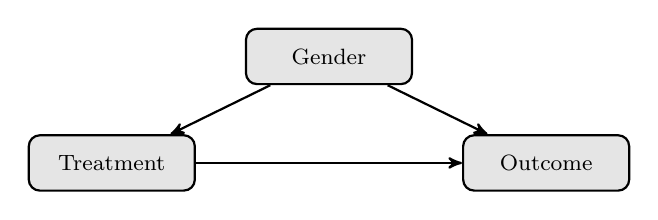
\begin{tikzpicture}[->,shorten >=0pt,shorten <=0pt,node distance=2.5em,thick,node/.style={observedrect},lt/.style={latent}]
\node[node](1){Gender};
\node[node, below left=of 1](2){Treatment};
\node[node, below right=of 1](3){Outcome};
\path[]
	(1) edge (2) edge (3) 
	(2) edge (3);
\end{tikzpicture}
\end{figure}

With this model, we see women are more likely to choose treatment $A$ and also more likely to recover regardless of what treatment they receive than men. Knowing a patient took drug A tells you they are much more likely to be female. When we compare the group of people who took A against those who took B, the greature proportion of females in the first group outweighs the higher benifit of drug B leading to an apparent reversal in effectiveness. However, when the doctor intervenes to set the treatment each person recieves there will no longer be a link from gender to treatment. So in this case she should choose which drug to prescribe from the gender specific table (and weight by the proportion of the population that belongs to each gender). Drug B is the better choice. 

\eqn{
\P{Y|do(T)} = \P{Y|T,female}\P{female}+ \P{Y|T,male}\P{male}
}

Is the solution to Simson's paradox to always to break down the data by as many variables as possible? No. Suppose we have the identical data as in \ref{tab:simpson1} and \ref{tab:simpson2} but replace the column name 'gender' with 'blood preassure', 'M' with 'high' and 'F' with 'normal'. This is a drug desined to prevent heart desease. One pathway to doing so might well be to lower blood preassure. Figure \ref{fig:simpsons_paradox2} shows a plausible causal graph for this setting. It differs from the graph in figure \ref{fig:simpsons_paradox} only in the direction of a single link. Now, however table \ref{tab:simpson2} tells us that people who took treatment $A$ had better blood preassure control and better overall outcomes. In this setting $\P{Y|do(T)} = \P{Y|T}$. Drug A is the better choice. 

\begin{figure}[h]
\caption{An example of Simpson's Paradox}
\label{fig:simpsons_paradox2}
\centering
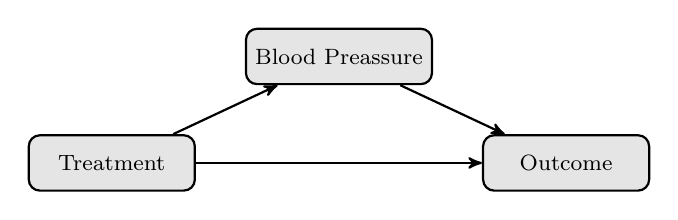
\begin{tikzpicture}[->,shorten >=0pt,shorten <=0pt,node distance=2.5em,thick,node/.style={observedrect},lt/.style={latent}]
\node[node](1){Blood Preassure};
\node[node, below left=of 1](2){Treatment};
\node[node, below right=of 1](3){Outcome};
\path[]
	(1) edge (3) 
	(2) edge (3)
	(2) edge (1);
\end{tikzpicture}
\end{figure}

Note that we have not changed the data itself, only the story we tell around it. This illustrates that the resolution to Simpson's paradox lies fundamentally not in the data itself but in what assumptions we are willing to make. From a purely statisitcal viewpoint there is no paradox. The reversal is just a case of INSERT VECTOR ARGUAMENT HERE. The 'paradox' only arises when we need to use the data to select an intervention. 

I should also point out that there are many other plausible causal graphs for both scenarios above. Perhaps income effects drug choice as well as gender, or gender could effect treatment choice and blood preassure control given treatment, etc. Causal modeling provides us with a powerful 



Human in the loop ML. Why would you need the human?

\todo{mention relationship to ecological fallacy}


\chapter{Two key questions}

We can roughly categorise the problems studied within causal inference into two groups, causal effect estimation and causal discovery. In causal effect estimation we assume (at least implicitly) that key aspects of the causal graph are known. The goal is then to estimate the causal effect of some action or range of actions. WHERE DOES MEDIATION FIT IN? THIS IS ALREADY HUGE, and is central to 1000 of papers published each year. Causal discovery aims to leverage much broader assumptions to learn the structure of causal graph from data. THIS IS THE AUTOMATION OF SCIENCE.

 
\section{Causal effect estimation} 

Causal effect estimation addresses the problem where we assume the key structure of the graph is known. That is, we assume that we have at a minimum:

\begin{itemize}
\item the target/outcome variable we care about
\item the focus/treatment variables on which we are considering interventions
\item any variables which act to confound two or more of the variables we have included.
\end{itemize}

Some of these variables my be latent or unobserved, in that we do not have measurements for them in the available data. However, their position in the network is assumed to be known. For example if we were interested in the effect of years of schooling on wages, we might expect that some measure of inherent ability could influence both the number of years of schooling people chose to pursue and the wages they subsequently obtain on graduating. Even if we have no data to directly measure peoples inherent ability, because it influences two of the variables were are modelling, we must include it in the graph.

Causal effect estimation is one of the most frequently applied methodologies within applied sciences. It implicit in millions of studies across medicine, business, economics and social sciences. Almost every time someone runs a regression model the key quantity of interest is a causal effect. Given how it underlies so much of our scientific progress, there is a enormous potential in properly understanding when we can draw causal conclusions, exactly what assumptions are required to do so and how we can best leverage those assumptions to infer as much information as we can from our data. 

\subsection{Mapping from observational to interventional distributions}
Once we have drawn the causal network for our problem, how can we use that to map information from the observational setting to the interventional one. Recall that a bayesian network is a way of representing the joint distribution over its variables in a way which highlights the any conditional independencies between them. 

\begin{theorem}
\textbf{(Local Markov condition)} Given a bayesian network $G$ with nodes $X_{1}...X_{N}$, each variable $X_{i}$ is independent of its non-decedents given its parents in $G$ for all distributions $P(X_{1}...X_{N})$ that are compatible with $G$.
\end{theorem}

The set of conditional independence relations given by the local Markov condition can enforce additional independencies that also hold in all distributions that are compatible with $G$. D-separation is an algorithm that extends the local Markov property to find these additional independencies. It provides us with a simple way of reading from a network if a given conditional independence statement is true in all distributions compatible with that network.

By leveraging conditional independencies we can effectively localise the effect of an intervention to a specific part of a larger graph. This gives rise to the do-calculus \cite{Pearl2000}. The do calculus consists of three rules. They derive from the causal information encoded in a causal network and the properties of d-separation and do not require any addition assumptions other than that of specifying the causal network. 

\subsubsection{Rule 1}
This rule describes which variables, on which we have not intervened, effect the distribution of the outcome given some intervention. The intervention $do(\boldsymbol{X}=\boldsymbol{x})$ changes a causal network, $G$, in a simple way. Variables in $\boldsymbol{X}$ are no longer determined by their parents but instead take on fixed values specified by $\boldsymbol{x}$. This corresponds to deleting the edges with arrows into variables in $\boldsymbol{X}$  (see figure \ref{fig:mutilatednet}). The resulting 'mutilated' network $G_{\overline{\boldsymbol{X}}}$ remains a causal network and d-separation still applies. 

If $(\boldsymbol{Y} \ci \boldsymbol{W} | \boldsymbol{Z},\boldsymbol{X})$ in $G_{\overline{\boldsymbol{X}}}$:
\begin{equation}
\label{eq:Do1}
 P(\boldsymbol{Y}|do(\boldsymbol{X}=\boldsymbol{x}),\boldsymbol{Z}=\boldsymbol{z},\boldsymbol{W}=\boldsymbol{w}) = P(\boldsymbol{Y}|do(\boldsymbol{X}=\boldsymbol{x}),\boldsymbol{Z}=\boldsymbol{z}) 
\end{equation}

$\implies$ if $(\boldsymbol{Y} \ci \boldsymbol{W} | \boldsymbol{X})$ in $G_{\overline{\boldsymbol{X}}}$:
\begin{equation}
\label{eq:Do12}
 P(\boldsymbol{Y}|do(\boldsymbol{X}=\boldsymbol{x}),\boldsymbol{W}=\boldsymbol{w}) = P(\boldsymbol{Y}|do(\boldsymbol{X}=\boldsymbol{x})) 
\end{equation}

This stems directly from the fact that the relationship between d-separation in a network and independence in the corresponding probability distribution still holds in the mutilated network. 

\begin{figure}[h]
\centering
\caption{Intervention in a causal bayesian network}
\label{fig:mutilatednet}
\begin{subfigure}[t]{0.3\textwidth}
\centering
\caption{original network, $G$}
\label{fig:mutilatedOriginal}
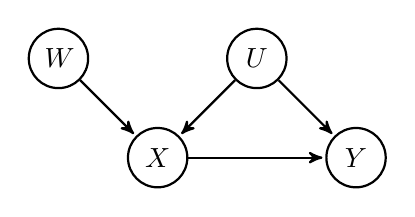
\begin{tikzpicture}[->,>=stealth',shorten >=1pt,auto,node distance=1cm,
  thick,main node/.style={punkt}]

 %nodes
\node[main node](1){$U$};
\node[main node, below left=of 1](2){$X$};
\node[main node, below right=of 1](3){$Y$};
\node[main node, above left=of 2](4){$W$};


 \path[every node/.style={font=\sffamily\small}]
    (1) edge node {} (2)
    	edge node {} (3)
    (2) edge node {} (3)
    (4) edge node {} (2);
	
\end{tikzpicture} 
\end{subfigure}
\begin{subfigure}[t]{0.5\textwidth}
\centering
\caption{network after the intervention $do(X=x)$, $G_{\overline{X}}$}
\label{fig:mutilatedAfter}
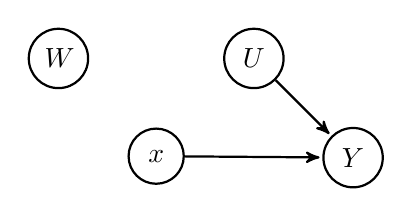
\begin{tikzpicture}[->,>=stealth',shorten >=1pt,auto,node distance=1cm,
  thick,main node/.style={punkt}]

 %nodes
\node[main node](1){$U$};
\node[main node, below left=of 1](2){$x$};
\node[main node, below right=of 1](3){$Y$};
\node[main node, above left=of 2](4){$W$};


 \path[every node/.style={font=\sffamily\small}]
    (1) edge node {} (3)
    (2) edge node {} (3);
    
\end{tikzpicture}
\end{subfigure}
\end{figure}

\subsubsection{Rule 2}
Rule 2 states when conditioning on $\boldsymbol{X} = \boldsymbol{x}$ and intervening  $do(\boldsymbol{X}=\boldsymbol{x})$ have the same effect on the distribution of the outcome $\boldsymbol{Y}$. You can think of this as when correlation is causation. It is easiest to understand by explicitly including the intervention process in the graphical model. We can depict the possibility of intervention by adding a new decision node $\hat{X}$ as a parent of each $X$ in the set of nodes we are intervening on (figure \ref{fig:augmentedNetwork}). Let $\epsilon$ be some arbitrary value not in the set of possible values for $X$. If $X = \epsilon$ the distribution of $X$ is what it was without intervention. Otherwise, if $X=x$, $X$ deterministically takes the value $x$ and is independent of its previous parents, representing the intervention $do(X=x)$. We use the notation $G^{\dagger}$ to represent $G$ augmented with these decision nodes. 

if $(\boldsymbol{Y} \ci \boldsymbol{\hat{X}}|\boldsymbol{X},\boldsymbol{Z},\boldsymbol{W})$ in $G^{\dagger}_{\boldsymbol{\overline{Z}}}$:

\begin{equation}
\label{eq:Do2}
P(\boldsymbol{Y}|do(\boldsymbol{Z}=\boldsymbol{z}),do(\boldsymbol{X}=\boldsymbol{x}),\boldsymbol{W}=\boldsymbol{w}) = P(\boldsymbol{Y}|do(\boldsymbol{Z}=\boldsymbol{z}),\boldsymbol{X}=\boldsymbol{x},\boldsymbol{W}=\boldsymbol{w})
\end{equation}

$\implies$ if  $(\boldsymbol{Y} \ci \boldsymbol{\hat{X}}|\boldsymbol{X})$ in $G^{\dagger}$:
\begin{equation}
\label{eq:Do22}
P(\boldsymbol{Y}|do(\boldsymbol{X}=\boldsymbol{x})) = P(\boldsymbol{Y}|\boldsymbol{X}=\boldsymbol{x})
\end{equation}

If the outcome does not depend on how the decision to assign the interventional variables was made, then the interventional distribution equals the observational one. 

\begin{figure}[h]
\centering
\caption{Augmented causal network with intervention}
\label{fig:augmentedNetwork}
\begin{subfigure}[t]{0.4\textwidth}
\centering
\caption{original network, $G$}
\label{fig:augmentedOriginal}
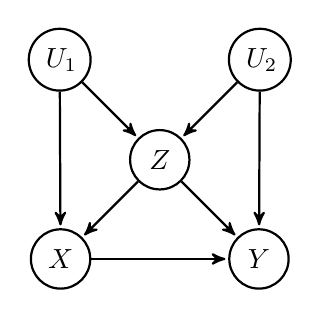
\begin{tikzpicture}[->,>=stealth',shorten >=1pt,auto,node distance=1cm,
  thick,main node/.style={punkt}]
 %nodes
\node[main node](1){$Z$};
\node[main node, below left=of 1](2){$X$};
\node[main node, below right=of 1](3){$Y$};
\node[main node, above left = of 1](4){$U_{1}$};
\node[main node, above right = of 1](5){$U_{2}$};


 \path[every node/.style={font=\sffamily\small}]
 	(2) edge node {} (3)
 	(4) edge node {} (2)
 		edge node {} (1)
 	(5) edge node {} (3)
 		edge node {} (1)
 	(1) edge node {} (2)
 		edge node {} (3);
    
	
\end{tikzpicture} 
\end{subfigure}
\begin{subfigure}[t]{0.4\textwidth}
\centering
\caption{augmented network after the intervention $do(Z=z)$, $G^{\dagger}_{\overline{Z}}$}
\label{fig:augmentedAfter}
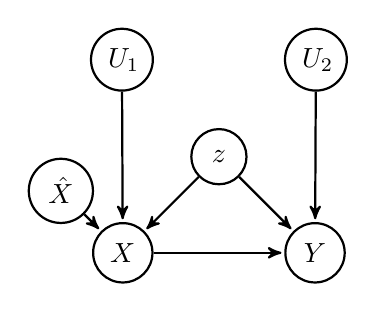
\begin{tikzpicture}[->,>=stealth',shorten >=1pt,auto,node distance=0.3cm,
  thick,main node/.style={punkt}]

\node[main node](1){$z$};
\node[below left=of 1](2){};
\node[below right=of 1](3){};
\node[main node, below left=of 2](4){$X$};
\node[main node, below right=of 3](5){$Y$};
\node[above right=of 1](6){};
\node[above left=of 1](7){};
\node[main node, above left=of 7](8){$U_{1}$};
\node[main node, above right=of 6](9){$U_{2}$};
\node[main node, above left=of 4](10){$\hat{X}$};


 \path[every node/.style={font=\sffamily\small}]
 	(4) edge node {} (5)
 	(10) edge node {} (4)
 	(8) edge node {} (4)
 	(9) edge node {} (5)
 	(1) edge node {} (4)
 		edge node {} (5);
 	
    
\end{tikzpicture}
\end{subfigure}
\end{figure}

\subsubsection{Rule 3}
This rule describes cases where the intervention $do(\boldsymbol{X}=\boldsymbol{x})$ has no effect on the distribution of the outcome $\boldsymbol{Y}$. 

if $(\boldsymbol{Y} \ci \boldsymbol{\hat{X}} |\boldsymbol{Z},\boldsymbol{W})$ in $G^{\dagger}_{\boldsymbol{\overline{Z}}}$:
\begin{equation}
\label{eq:Do3}
P(\boldsymbol{Y}|do(\boldsymbol{Z}=\boldsymbol{z}),do(\boldsymbol{X}=\boldsymbol{x}),\boldsymbol{W}=\boldsymbol{w}) = P(\boldsymbol{Y}|do(\boldsymbol{Z}=\boldsymbol{z}),\boldsymbol{W}=\boldsymbol{w})
\end{equation}
$\implies$ if  $(\boldsymbol{Y} \ci \boldsymbol{\hat{X}})$ in $G^{\dagger}$:
\begin{equation}
\label{eq:Do32}
P(\boldsymbol{Y}|do(\boldsymbol{X}=\boldsymbol{x})) = P(\boldsymbol{Y})
\end{equation}
The statement that $\boldsymbol{Y} \ci \boldsymbol{\hat{X}}$ without conditioning on $\boldsymbol{X}$ implies that there is no unblocked path from $\boldsymbol{X}$ to $\boldsymbol{Y}$ which starts on an arrow leaving $\boldsymbol{X}$. This means there is no causal effect of $\boldsymbol{X}$ on $\boldsymbol{Y}$ and the intervention $do(\boldsymbol{X}=\boldsymbol{x})$ does not alter the distribution of $P(\boldsymbol{Y})$.

\subsection{Identifiability}
A natural question to ask is, given the level of assumptions we have made about the graph, is it possible to estimate a causal effect from observational data? This is the identifiablity problem. Identifiability is an asymptotic property of the graph. It asks if we can obtain an unbiased point estimate for the causal effect of interest in the infinite data limit. A problem is non-parametrically identifiable if it is identifiable without any additional assumptions on the functional form of the dependencies between variables in the graph. 

The question of non-parametric identifiability is solved! The do calculus is complete. A problem is identifiable if and only if the interventional distribution of interest can be transformed into term containing only observational quantities via repeated application of the do calculus. 

There is an algorithm \cite{Shpitser2012} based on these properties that, for a given network and interventional (do-type) query, can:

\begin{enumerate}
\item determine if the query can be translated into an expression involving only distributions over observed variables. In other words, determine if the query is identifiable given the assumptions encoded by the network
\item if it is identifiable, return the required expression 
\end{enumerate}

\todo{insert link to working javascript version}
\todo{figure with typical examples}

There are many interesting questions relating to identifiability that remain open. What is the minimal (by some metric) additional information that would be required to make a non-identifiable query identifiable? What if we assume various restrictions on the functional form of the relationships between the variables? Clearly  . A complete algorithm for the problem of linear identifiability is yet to be found, despite a rich body of work going back to at least ??? \ref{}

Is identifiablity a good question to ask? It seems natural to see if a problem can be solved with infinite data before we try to see how well we can do it with finite data. However, we should not give up on non-identifiable problems. We may still be able to achieve useful bounds on causal effects with finite data even if point estimation is not possible. From that perspective we should be cautious about dividing problems into identifiable and not identifiable. 

How do we tackle a problem that is not identifiable. We could look for bounds or we could make additional assumptions (or both). 

\subsection{Estimation}
\subsubsection{Defining causal effects} 
So far we have described causal effect estimation in term of identifying the interventional distribution $\P{Y|do(X)}$ from observational data. 

From a decision making process, is it the right thing to do to just pick the X that maximises the expectation of $Y$ (assuming that higher $Y$ is better. If it is not we can just add in another variable that is a deterministic function of $Y$ to relect the loss function.)

Typically however we are often interested in estimating some function of the difference between $P{Y|do(X)}$ for various values of $X$. For example, the average causal effect (ATE) is defined for discrete binary treatment $T$ by:

\eqn{
ATE = \E{Y|do(T = 1)} - \E{Y|do(T=0)}
}

If the variables are continuous the average casual effect is 

\todo{insert equation for continuous case}

The individual causal effect as defined in section XXX cannot be stated in terms of the do notation as it is not with respect to a distribution over anything. However, we can define a very similar concept with respect some observed context which I will refer to as the personalised causal effect. 

\todo{insert equation for personalised causal effect}

However, the difference in expectation is not the only way of summarising the difference between two (or more) distributions. \citep{Janzing2013} show that there is no single way of summarising the collection of distributions represented by $\P{Y|do(X)}$ that satisfies a number of reasonable axioms. 

An obvious alternative to subtracting the exceptions would be to consider ratio. Is there any reason that we don't do this that relates to the argument in Dawid? What about the smoothness of any uncertainties?

\subsubsection{Estimating the difference when the back door criteria is met}

A very substantial number of practical studies fall into the category of causal inference via the backdoor theorem. A study is done. It is assumed that it is ignore-able. That is that we have a a set of variables satisfying the back door adjustment criteria. The goal is to estimate the average causal effect. Since we have assumed the backdoor criteria is met, the query is identifiable. Problem solved. Except we have finite data ...

What are the approaches for doing so? 

There are multiple ways of doing the adjustment. 

In order to block the path of spurious information it is sufficient to (perfectly) model either the treatment selection process $\P{T|Z}$ or the response function $\P{Y|T,Z}$. 

\paragraph*{matching}

\paragraph*{regression}
\paragraph*{When is regression causal?}
A regression equation is causal if, when we represent the equations as a bayesian causal model or structural equation model, we claim the arrows are causal AND if the variables we include in the regression form a valid back door adjustment set. 


\paragraph*{propensity scores}

They have advantages and disadvantages depending on the setting. Methods like regression typically impose a parametric model of some description onto the treatment assignment or response function. 

- Connection of nearest matching to nearest neighbour. 

Once we have made the assumptions required to define the causal graph and identify a valid adjustment set, is there any difference between the causal effect estimation problem and standard supervised machine learning. 

\cite{causal estimation is covariate shift}

However, there is a critical remaining complication. In supervised learning we can split our data into training and validation data sets or apply cross validation to select models and model parameters. In the causal estimation case we cannot. We lack samples from the counterfactual. 

The significance to this should not be underestimated. Cross-validation has allowed applied machine learning to proceed with very a theoretical approach on the basis that we can identify when a model is successful. With causal effect estimation there is no guarantee that a model which performs well at prediction (even out of sample) will accurately estimate the outcome of an intervention. 

GIVE A CONCRETE EXAMPLE here. One would be a model which looks at a post-treatment variable in order to make predictions. But what about if we assume the model structure is correct and known.  Can we fit parameters that do better on prediction but worse on casual effect estimation?

\cite{Imbens2004} Review of non-parametric estimation

Discuss the recent competition on this question and the results

Discuss the role that the models used to simulate the data may have in determining which models perform the best. 

\subsection{Non identifiable queries}
In many cases the query of interest will not be identifiable. In this setting we are left with a choice between making additional assumptions (for example that variables are linearly related) or aiming to obtain bounds rather than point estimates for the causal effect of interest. Or we may do both. One of the most widely used methods in this category is the instrumental variable. 

Instrumental variables are often conceptualised as natural experiments. The goal is to find a variable that substantially influences the treatment but that is conditionally independent of the remaining variables in the network. 

For example, we might want to compare the results for juvenile offenders depending on whether they spent their time awaiting trial in a custom facility for young offenders as opposed to a unit within an adult jail. The process by which children are assigned to different facilities may well be non-random. However, it might be that in many cases the decision was based purely on the fact that the juvenile facility was full. We could then use the number of places remaining in the juvenile facility as an instrumental variable. 

The causal network for an ideal instrumental variable is shown in figure XXX. It is not identifiable (non-parametrically) because. If we assume linearity it ? \todo{what exact guarantees do we get for instrumental variables}. Without a linearity assumption we would want the instrumental variable to be highly predictive of the treatment assignment so as to obtain reasonable bounds. But if we make the assumption that everything is linear then it would seem that even a weak instrumental variable should (in theory) suffice. 

In some cases we might have a choice between adjusting for causal effects via the backdoor theorem or utilising an instrumental variable to obtain bounds. It is not the case that the former method is always superior even though it has better asymptotic results. For example 

DEMONSTRATE a specific example where instrumental variables obtain better estimates than adjustment even when all the criteria for adjustment have been met. Start with a case were the adjustment is very high dimensional and the instrumental variable is strong. (the effect of the variables on the treatment assignment will have to be week (otherwise the instrument is not strong). 


\subsection{How successful overall is causal effect estimation}
Really know one knows.

There are relatively few studies that have compared the observational study results with those obtained by randomised experiments. One of the key examples is the XX job network study. Initial analysis suggested that a range of causal estimation techniques all ...

\paragraph*{How can we construct data sets on which to test casual effect estimation techniques}
One can start from a randomised experiment and deliberately drop some of the data. Draw up the graphical model for this process and the assumptions inherent in it. 

\section{Causal Discovery}

Cyclic models \cite{Hyttinen2012}

We now move to the much more general problem of learning a causal graph from observational data. In this setting we make much broader assumptions about the structure of the graph. For example, that it is acyclic or that we have no unmeasured confounding variables. We do not assume the existence or directions of any links between the variables. Amazingly, it is possible to infer some aspects of causal structure with such general assumptions. The set of conditional independence in a non-experimental data set indicates some causal structures are more likely than others. In addition, there can be subtle asymmetries in the relationship between the joint distribution of cause and effect and the distributions of cause given effect and effect given cause. These clues are the key to causal discovery algorithms.

There is also work on inferring causal structure from experiential data \ref{}. We discuss this further in section XXX.

Causal discovery is a much grander goal than causal effect estimation given a known causal network. Arguably, if achieved, it would equate to the automation of scientific discovery. We need simply supply our algorithm with a vast collection of variables (regardless of their relevance to the problem) and it would learn the causal structure and from that allow us to estimate the effects of any intervention we cared to make. Unfortunately, causal discovery is very hard. Even with the assumption that the causal graph is acyclic and there are no latent variables, the number of possible graphs grows XXX exponentially (or super-exponentially)? with the number of variables. - some intuition here about the strength of the signal we get from causal discovery. Small initial errors in greedy approaches can cascade leading to unstable inference and large losses \ref{sprites?}. Talk about the numerical as well as the statistical issues here. 

In the next sections we briefly survey the key approaches to causal discovery. We roughly divide the methods into those based on those that exploit the connection between the conditional independencies in a joint distribution and the structure of a causal model and those that leverage assumptions about the functional form of the relationships between cause and effect. This is not the only way we could have grouped them. There is also a separation between constraint based algorithms, that XXXX and those that search and score multiple graph structures before selecting the best. There are also hybrid methods \ref{}  

\subsection{Conditional independence based methods}
One general approach is to look for clues about the structure of the network in the conditional independence relations in the distribution. For any bayesian network, $G$, (causal or not) we can read of conditional independencies in the joint distribution from the structure of the network. If a set of variables $Z$ d-separates $X$ and $Y$ in $G$ then $(X \ci Y|Z)$ in the distribution $P$. However, we want to work in the other direction, from conditional independence in the distribution to the structure of the network. This requires that we assume the reverse condition: $(X \ci Y|Z)$ in $P$ must imply $Z$ d-separates $X$ and $Y$ in $G$. This assumption, commonly referred to as  \textbf{\textit{faithfulness}} \ref{}, says there are no additional independence relations that are satisfied in $P$ but not in all distributions $\boldsymbol{P'}$ that are compatible with $G$. Stating that $P$ is faithful to $G$ is equivalent to $G$ is a \textbf{\textit{perfect map}} \cite{Kollner} for $P$.

Faithfulness is an assumption. It does not always hold and we cannot verify it from the observational data we wish to use for causal inference. However, most distributions generated by a causal bayesian network will be faithful to that network. For faithfulness to be violated, different causal effects must exactly balance one-another out. For example, consider a simple binary variable model of chocolate consumption, income and obesity (figure). If the coefficients in the conditional probability tables are just right then the direct effect of chocolate on obesity will exactly balance the indirect effect through income and obesity will appear independent of chocolate consumption. However, this independence is not stable. It would disappear under a small perturbation to any of the parameters. \todo{point out violations are solutions to polynomial equations and thus measure 0 \ref{XX}}  

Given the faithfulness assumption, our causal discovery problem reduces to finding the set of bayesian networks that have exactly the dependency structure as we observe in $P$. This set can also be referred to as the Markov equivalence class compatible with $P$.

\subsubsection{Without hidden common causes}
The strong assumption that there are no hidden variables that cause two or more variables in $\boldsymbol{V}$ significantly reduces the 'search space' of bayesian networks we must consider. 

We will begin with a brute force algorithm (described as the SGS algorithm in \cite{Sprites} and IC algorithm in \cite{Pearl2000}). While it is impractical for all but the smallest of networks, it demonstrates key concepts that also underlie the more useful and complex algorithms we will discuss later. 

\begin{table}[H]
 \begin{tabularx}{\textwidth}{X}
 \hline
\rule{0pt}{2.5ex} 
 \textbf{The SGS (or IC) Algorithm}\\
 \hline
 \rule{0pt}{2.5ex}
\textbf{Input:} A distribution $P$, over variables $\boldsymbol{V}$, that was generated by and is faithful to an (unknown) bayesian network $G$\\
\textbf{Output:} A partially directed network that represents the Markov equivalence class of $G$\\
 \begin{enumerate}[itemsep=8pt]
  \item Join all pairs of vertices $(a,b) \in \boldsymbol{V}$ with an un-directed link to form a complete graph.
  \item For each link $a-b$ search for a set $\boldsymbol{S}_{a,b} \subseteq V \setminus \{a,b\}$ that renders $a$ and $b$ conditionally independent. If such a set (including the empty set) exists then $a$ and $b$ cannot be directly connected in $G$ so delete the link.
  \label{alg:SGSexponential}
  
  \item For all pairs of non-linked variables $(\alpha,\beta)$ with a common neighbour, $c$, if $c \notin \boldsymbol{S}_{\alpha,\beta}$, then $c$ must be a collider in the path $\alpha,c,\beta$ so  add arrows to direct the links $\alpha-c$ and $\beta-c$ towards $c$.
  \label{alg:SGScolliders}  
  \item Recursively try to orient any edges that remain un-directed to avoid creating cycles (because they are not there by assumption) and additional colliders (because any colliders were found in step \ref{alg:SGScolliders}).
  \label{alg:SGSfinal}
\end{enumerate}\\
 \hline
\end{tabularx}
\end{table}

The SGS algorithm utilises the fact that a collider structure (figure \ref{fig:dseptripple4}) induces a distinct conditional independence relation. Assuming you have a consistent conditional independence test, it converges to return a partially directed network that represents the Markov equivalence class for the generating causal model. Unfortunately the number of conditional independence tests required for step \ref{alg:SGSexponential} grows exponentially (in the worst case) with the number of variables. Not only that, but for each edge that is in the true network, the algorithm will always tests all other possible subsets of variables. If the assumption that there are no hidden common causes or that the distribution is faithful are violated, step \ref{alg:SGScolliders} of the SGS algorithm can produce double headed arrows.

The PC algorithm \cite{Sprites} modifies step \ref{alg:SGSexponential} of the SGS algorithm to utilise the fact that if two variables $(a,b)$ are conditionally independent given some set, they will also be conditionally independent given a set that contains only variables adjacent to $a$ or $b$. It also checks for low order conditional independence relations before higher order ones. This allows it to exploit any sparsity in the true network, leading to much better average case performance  \cite{Sprites} (although the worst case, where the true network is complete, is still exponential). With finite data, the order in which the links are considered can change the output (unlike for SGS). The effect of wrongly removing a link early on flows through to later conditional independence tests by changing which nodes are considered adjacent.


\begin{table}[H]
 \begin{tabularx}{\textwidth}{X}
 \hline
\rule{0pt}{2.5ex} 
 \textbf{The PC Algorithm}\\
 \hline
 \rule{0pt}{2.5ex}
\textbf{Input:} A distribution $P$, over variables $\boldsymbol{V} = \{V_{1}...V_{k}\}$, that was generated by and is faithful to an (unknown) bayesian network $G$\\
\textbf{Output:} A partially directed network that represents the Markov equivalence class of $G$\\
 \begin{enumerate}[itemsep=8pt]
  \item As for SGS
  \item \textbf{for} each link $a-b$:
  \begin{itemize}[label={}]
   \item $n = 0$
   \item $\boldsymbol{A}_{a,b} = \{A_{1}...A_{j}\}$ be the set of nodes adjacent to $a$ and/or $b$
   \item \textbf{while} $a$ and $b$ are connected and $n < j$:
   \item 
    	\begin{itemize}[label={}]
    	\item \textbf{if} any subset of size $n$ of $\boldsymbol{A}$ makes $a$ and $b$ conditionally independent:
    	\item \begin{itemize}[label={}]
    			delete the link
    		  \end{itemize}
    	
    	\item $n = n+1$
    	\end{itemize}
  \end{itemize}   
  \item as for SGS
  \item as for SGS
\end{enumerate}\\
 \hline
\end{tabularx}
\end{table}

The PC algorithm also returns a set of Markov equivalent networks consistent with the distribution. Since we have assumed there are no hidden variables, for any single graph in this set we can calculate causal effects with equation \ref{eq:allvarsobserved}. We can then bound the true causal effect by combining the results for the all the networks. This procedure is the IDA algorithm \cite{Maathuis2009} and has been found to outperform standard regularisation techniques at finding causal effects in a high-dimensional yeast gene expression data set \cite{Maathuis2010}. An implementation is available in the R package \cite{Kalisch2012} 

\todo{mention failed replication - if published}

\subsubsection{With hidden variables}
There are an number of difficulties in extending the approach of the last section to deal with the case where there are latent variables. With an unknown number of hidden variables there are infinity many possible structures to search over. In addition, the space of causal networks is not closed under marginalisation. If we have a distribution that $P'(\boldsymbol{O},\boldsymbol{U})$ generated by and is faithful to a network $G$ the distribution $P(\boldsymbol{O})$, that results from marginalising over $\boldsymbol{U}$, may not be faithful to any bayesian network (see figure \ref{fig:DAGSnotclosed}).

\begin{figure}
\centering
\caption{A distribution faithful to this DAG is not faithful to any DAG over the variables $\{A,B,C,D\}$ after marginalising over $U$. }
\label{fig:DAGSnotclosed}
 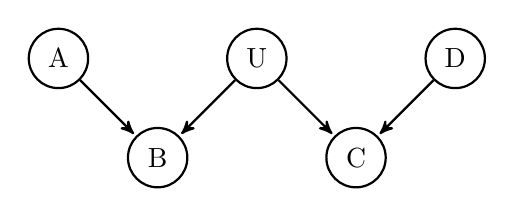
\begin{tikzpicture}[->,>=stealth',shorten >=1pt,auto,node distance=1cm,  thick,main node/.style={punkt}]
 %nodes
\node[main node](1){U}; 
\node[main node, below left = of 1](2){B};
\node[main node, below right = of 1](3){C};
\node[main node, above left= of 2](4){A};
\node[main node, above right = of 3](5){D};

 \path[every node/.style={font=\sffamily\small}]
    (1) edge node {} (2)
    	edge node {} (3)
    (4) edge node {} (2)
    (5) edge node {} (3);
    	
\end{tikzpicture}
\end{figure}
 

The key to constraining the space of possible models is that many latent structures are equivalent (under transforms of the hidden variables). See example figure XXX.

\begin{theorem}
\cite{Verma1993} For every latent structure there is a dependency equivalent structure such that every latent (unobserved) variable is a root node with exactly two children .
\end{theorem}

Since we only care about the causal relationships between observed variables, it is sufficient to search over networks where any hidden variables have no parents and directly cause two of the observed variables. Instead of representing hidden variables explicitly we can capture the necessary independence relations with a more general graphical model that supports bi-directed edges that play the role of a hidden confounding variable. These models, referred to as maximal ancestral graphs (MAGs) are closed under marginalisation and conditioning. 

For any DAG with latent (and selection) variables there is a unique MAG \cite{Richardson2002}. This makes it possible to extend the PC algorithm to latent structures, resulting in the FCI algorithm \cite{Sprites}. The logic behind the algorithm is very similar. Certain structures are ruled out as a consequence of being inconstant with the observed conditional independence relations. The output is an equivalence class of MAGs, which can be represented graphically as a partial ancestral graph PAG. Assuming there are no selection variables (see \cite xxx), the PAG can contain four types of link:

\begin{enumerate}
\item $X \rightarrow Y$, meaning $X$ causes $Y$
\item $X \leftrightarrow Y$, meaning there is a latent variable that causes $X$ and $Y$.
\item $X\ {\circ} {\rightarrow}\ Y$, either $X$ causes $Y$ or a latent variable causes both.
\item $X\ {\circ} {-}  {\circ}\ Y$, either $X$ causes $Y$ or $Y$ causes $X$ or a latent variable causes both.
\end{enumerate}

The circles indicate where it is ambiguous if there should be an arrowhead (ie where there is one in some MAGs and not in others in the equivalence class). Counter-intuitively it is sometimes possible to  rule out or confirm the existence of a confounding variable and fully determine the causal type of a link (see examples in figure \ref{fig:FCIExamples}). 


\todo{put these figures in a table with true graph input on left and FCI output on right}
\todo{uniform styles used for nodes across thesis}
\begin{figure}
\centering
\caption{FCI examples: true graph and FCI output}
\label{fig:FCIExamples}
 \begin{subfigure}[t]{0.8\textwidth}
 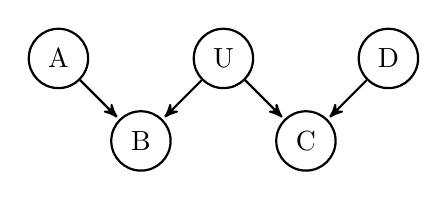
\begin{tikzpicture}[->,>=stealth',shorten >=1pt,auto,node distance=.7cm,  thick,main node/.style={punkt}]
 %nodes
\node[main node](1){U}; 
\node[main node, below left = of 1](2){B};
\node[main node, below right = of 1](3){C};
\node[main node, above left= of 2](4){A};
\node[main node, above right = of 3](5){D};

 \path[every node/.style={font=\sffamily\small}]
    (1) edge node {} (2)
    	edge node {} (3)
    (4) edge node {} (2)
    (5) edge node {} (3);
    	
\end{tikzpicture}
 \end{subfigure}
 \begin{subfigure}[t]{0.8\textwidth}
 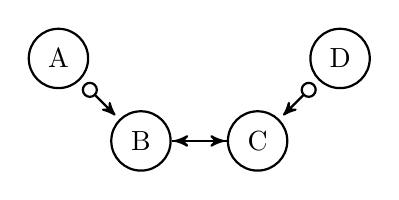
\begin{tikzpicture}[->,>=stealth',shorten >=1pt,auto,node distance=.7cm,  thick,main node/.style={punkt}]
 %nodes

\node[main node](1){A};
\node[main node, below right=of 1](2){B};
\node[main node, right=of 2](3){C};
\node[main node, above right=of 3](4){D};

 \path[every node/.style={font=\sffamily\small}]
    (1) edge[pil] node {} (2)
    (2) edge node {} (3)
    (3) edge node {} (2)
    (4) edge [pil] node {} (3);    	
\end{tikzpicture}
\end{subfigure}
 \begin{subfigure}[t]{0.4\textwidth}
 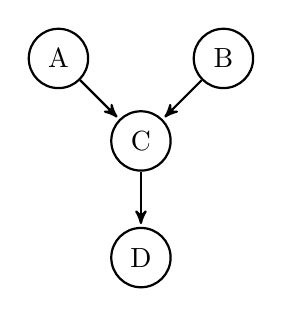
\begin{tikzpicture}[->,>=stealth',shorten >=1pt,auto,node distance=0.7cm,  thick,main node/.style={punkt}]
 %nodes

\node[main node](1){C};
\node[main node, above left=of 1](2){A};
\node[main node, above right=of 1](3){B};
\node[main node, below=of 1](4){D};

 \path[every node/.style={font=\sffamily\small}]
    (1) edge node {} (4)
    (2) edge node {} (1)
    (3) edge node {} (1);    	
\end{tikzpicture}
\end{subfigure}
 \begin{subfigure}[t]{0.4\textwidth}
 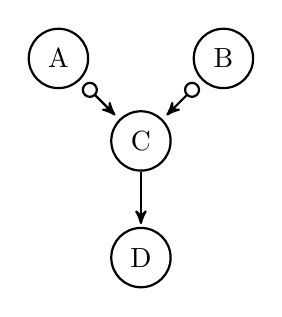
\begin{tikzpicture}[->,>=stealth',shorten >=1pt,auto,node distance=0.7cm,  thick,main node/.style={punkt}]
 %nodes

\node[main node](1){C};
\node[main node, above left=of 1](2){A};
\node[main node, above right=of 1](3){B};
\node[main node, below=of 1](4){D};

 \path[every node/.style={font=\sffamily\small}]
 	(1) edge node {} (4)
    (2) edge [pil] node {} (1)
    (3) edge [pil] node {} (1);    	
\end{tikzpicture}
\end{subfigure}
\end{figure} 

The FCI algorithm can be made complete such that it discovers all aspects of the true causal structure that are identifiable from the conditional independence relations of a distribution over observed variables and the faithfulness assumption \cite{Zhang2008}. More recently \cite{Colombo2012} have proposed the RFCI algorithm, which in some cases returns more ambiguous links than FCI but is substantially faster. \cite{Claassen2013} point out that the problem of learning sparse causal networks from data is not NP-hard and propose the FCI+ algorithm, that requires $O(N^{2(k+2)})$ conditional independence tests, where $k$ is the maximum node degree over the observed variables. 

With latent variables we are not using all the information - so we could go further (to nested Markov models and inequalities.) \cite{Richardson2012} \cite{Shipster2014}


These are all constraint based methods ... efficient because they stop early, but also may not be robust to errors early on. 

A comparison of algorithms 

\renewcommand{\arraystretch}{1.5}
\begin{tabular}{| c | c | p{4cm} | c | c | c |}
\hline
  \textbf {Alg.} &\textbf{ Method }& \textbf{Scales (num.vars) }& $\sim $ \textbf {Vars} & \textbf {Latent } & \textbf {Reference} \\
  \hline
  IC/SGS & Constraint based & Exponential & 10 & No & Pearl(2000)/Sprites(2000)\\
  \hline
  PC & Constraint based & Worst case exponential, polynomial for sparse graphs & 5000 & No & Sprites(2000) \\ 
  \hline
  FCI & Constraint based & Worst case exponential, polynomial variant FCI+ for sparse graphs & 30 & Yes & Sprites(2000) \\
  \hline
  RFCI & Constraint based & ? & 500 & Yes & Colombo(2012) \\
  \hline
  GES & Search \& Score  & Worst case exponential & 50 & No & Chickering(2002) \\
  \hline
  MMHC & Hybrid & ? & 5000 & No & Tsamardinos(2006) \\
 \hline
\end{tabular}

\subsubsection{Doing conditional independence tests}

All the algorithms we have discussed in the previous section rely on being able to perform conditional independence tests. This is non-trivial with high dimensional data. If the functional relationship between the variables is linear with Gaussian noise then the network represents a multivariate normal distribution and a pair of variables $A$ and $B$ are conditionally independent if and only if the corresponding entry in the inverse correlation matrix is non-zero. Where the functions are non-linear 

\begin{itemize}
\item \cite{Zhang2012} Kernel independence tests
\item HSIC \cite{Gretton2008}
\end{itemize}

\subsection{Discovery with functional models}
The algorithms we have considered so far return a Markov equivalence class. They cannot distinguish between two models that result in the same set of conditional independence relations. Consider the very simple case where we have only two variables and the only possible causal structures are $X \rightarrow Y$ or $Y \rightarrow X$. These models have the same dependency structure but in one case $P(Y|do(X)) = P(Y|X)$ and in the other $P(Y|do(X)) = P(Y)$. No algorithm relying purely on conditional independence relations can separate these two cases. 

Let us focus only on the two variable case $X \rightarrow Y$ or $Y \rightarrow X$. What possible clues could there be in the distribution $P(X,Y)$ that could indicate which causal model it was generated from. Recall the functional definition of causality (section \ref{sec:SEM}). There are a number of assumptions about the form of the functions that can allow us to identify the causal direction: non-invertible functions, additive noise \cite{Hoyer2009}, post-non-linear additive noise \cite{Zhang2008a}, linear models with non-Gaussian noise \cite{Hoyer2012}

There is a connection between casual discovery and semi-supervised learning.\cite{causal anti causal}. Suppose we are trying to learn $\P{Y|X}$. The goal of semi-supervised learning is to improve our estimate of $\P{Y|X}$ by leveraging additional data sampled from $\P{X}$. However, if the true causal model is $X \rightarrow Y$ then their is some function mapping values of $X$ to $Y$ which should be invariant to any changes in the input distribution $\P{X}$. Therefor $\P{X}$ should be independent of $\P{Y|X}$ and semi-supervised learning should not perform any better than standard supervised learning. However if the true causal model is $Y \rightarrow X$ then variations in the $P{X}$ can result from both the input distribution over $Y$ and the mapping from $X$ to $Y$ and semi-supervised learning could help.

ONE POINT I'M NOT CERTAIN ON HERE. might not knowledge of $\P{X}$ help define which region of the mapping we need to be most accurate on in order to minimise the loss (ie analogous to the covariate shift problem). \todo {open question}

%If X → Y, what is the relationship between P(X) and P(Y|X)? 
What about P(Y) and P(X|Y)?

%In semi supervised learning we are given training points from P(X,Y) and additional points sampled from P(X). The goal is to learn P(Y|X). The extra points from P(X) will not help if X → Y.

deterministic functions,

IGCI \cite{Janzing2012a}

Independence of input and mechanism. Daniusis et al 2012

Independence of function and input: If $X \rightarrow Y$ and we have a functional causal model $y = f(x,e)$ then the input
distribution $P(X)$ and function $f$ represent independent mechanisms. We do not expect a change in the input distribution to modify the function. 


Instead of positing a functional restriction on the relationship between variables and then developing theory to exploit that assumption, \citep{LopezPaz2014} propose learning what the causal relationship looks like from data. They assume there will be a difference between the relationship of $\P{X}$, $\P{Y}$ and $\P{X|Y}$ between $X \rightarrow Y$ versus $Y \rightarrow X$. Their algorithm requires a data set in which each row is itself a data set consisting of pairs of variables $(x_i,y_i)$ with a label indicating the direction of causality between $X$ and $Y$. They use a kernel mean embedding to represent the distributions $\P{X}$, $\P{Y}$ and $\P{X|Y}$ as features for each individual sub-data set and train an algorithm to learn the direction of causality. Unfortunately we do not have a large collection of data sets where the causal direction is known to train such a model. \citep{LopezPaz2014} instead use a simulated data set so their model will necessarily be base on the assumptions they make when generating the data. Nonetheless this approach makes it possible to rapidly construct a model from a wide range of possible assumptions, without doing a lot of theory to design a specific algorithm optimised to that setting. Their approach performed well in the causal effect pairs challenge, correctly identifying the causal direction in ?? percent of cases (against a benchmark of 50\% from random guessing)\ref{XXX}.


\citep{Peters2014} have extended results from the bi-variate case to the multivariate setting (with no hidden variables)?. They show that if we can come up with a condition that guarantees identifiability for the bi-variate case, we can extend that result to get the conditions under which the multivariate case is identifiable. The build on this to develop an algorithm that allows the construction of causal graphs based on the additive assumption??

\subsection{Granger causality}

Granger causality was developed within economics and is not typically discussed within the causal discovery literature.  

Although it does differ from the previous approaches in the types of assumption it relies upon it none-the-less tackles the same goal 

so we shall include it here. 

Granger casualty essentially assumes that the future cannot cause the past. This may seem an entirely waterproof assumption. However it can be tripped up by unmeasured confounding variables. The cock crows before the sun rises - so does it cause the sun to rise? No. 



\chapter{The interventionist viewpoint}

The previous sections all focus on aspects of the question; how can we estimate the effect of an intervention in a system from data collected prior to taking it. There is an obvious alternative. Instead of trying to infer the outcome of an intervention from passive observations we could just do it and see what happens. There are two key differences between observing a system and explicitly intervening in it. Firstly, when we intervene, we can choose which actions to take and thus get some control over which distributions we learn about. Secondly, if we are explicitly choosing interventions, we have a perfect model of the probability that we select each action given any context, allowing us to control confounding bias. 

\subsection{The role of randomisation}
Randomised controlled trials are often presented as the gold standard for determining causal effects in many areas of social sciences and economics \ref{XXX}. What is it about randomisation that makes it so important when it comes to causality? The graphical model for a randomised controlled experiment is shown in figure \ref{fig:random_experiment_network}. If we assume perfect compliance (everyone takes the treatment that we select for them) then we have a perfect model for the treatment assignment process. Since treatment is assigned randomly, there can be no other variables that influence it and thus no confounding variables that effect both treatment and outcome. 

\begin{figure}[h]
\caption{causal network for a randomised experiment}
\label{fig:random_experiment_network}
\centering
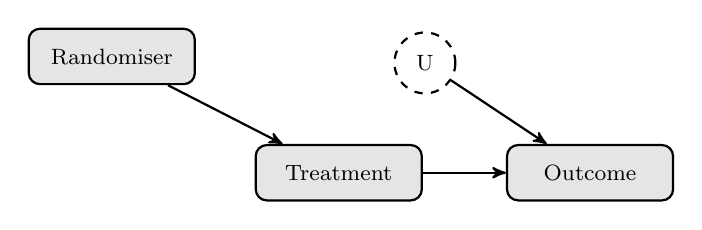
\begin{tikzpicture}[->,shorten >=0pt,shorten <=0pt,node distance=3em,thick, node/.style={observedrect}, lt/.style={latent}]
\node[node](1){Treatment};
\node[node, above left=of 1](2){Randomiser};
\node[node, right=of 1](3){Outcome};
\node[lt, above left=of 3](4){U};
\path[]
	(2) edge (1)
	(1) edge (3)
	(4) edge (3);
\end{tikzpicture}
\end{figure} 

\todo {turn this into something}
This would be a natural place to discuss what happens with finite data sets where there are many other variables that influence the outcome. We expect that across at least some of these variables, the target and control group will not be balanced. Does this not inject bias into the causal estimates? The answer is no, (I think - a better more general proof would be nice). The more such attributes there are, the higher is the variance in the outcome within the target and control group. When we perform a confidence test to ascertain whether or not there is a difference ... what happens.

Randomisation does not ensure target and control group are exactly alike. The more other features (observed or latent) influence the outcome, the more likely it is that there will be a significant difference in the joint distribution of these variables in a between the target and control groups in a finite data sample. However, the variance in the outcome within both the target and control groups also increases. The net result is increased variance (but not bias) in  the estimate of causal effects. 

DISCUSS STRATIFIED RANDOM EXPERIMENT

What is the role of randomisation? How do bandits algorithms work despite being only partially randomised? What else can you do to improve randomised studies (variance reduction, lower regret).

The benefit provided by randomisation in breaking the link between the treatment variable and any con founders should not be understated. The possibility of confounders cannot be empirically ruled out from observational data \citep{Pearl2000} (test for confounding). This means causal estimates from non-experimental data are always subject to the criticism that an important confounder may have been overlooked or not properly adjusted for. However, randomised experimentation does have some limitations. 

\subsubsection{Limitations of randomised experiments}
\label{subsec:limitations_of_experiment}
\begin{enumerate}

\item The probability that an individual is treated is set in advance and fixed over the course of the experiment. As the experiment proceeds we may start to see evidence that one treatment is much more effective than another. However (in a pure randomised experiment) we don't use this information to update the treatment that later patients revive. The result is that some will unessential be given a sub-optimal treatment. 
\item Experiments are expensive and difficult to conduct. This means experimental data sets are often much smaller than observational ones, limiting the complexity of models we can explore.

\item Experiments are often conducted on a convenient but unrepresentative sample of the broader population of interest (for example first year collage students at research universities). This can result in estimates with high \emph{internal validity} \citep{Campbell1963} in that they should replicate well in a similar population, but very low \emph{external validity}. The results may not carry over to the general population of interest. The question of whether an experiment conducted on one population can be mapped to another is referred to as the transportability problem \citep{Bareinboim2013} \todo{check ref} and relies on very similar assumptions and arguments to causal inference and the do-calculus. 

\item The idealised notion of an experiment represented by figure \ref{fig:random_experiment_network} does not capture the complexities of randomised experiments in practice. There may be imperfect compliance: the treatment selected by the randomiser is not always followed. Or output censoring: the experimenter is not able to observe the outcome for all units (for example if people drop out). If compliance or attrition is not random but associated with (potentially latent) variables that also effect the outcome then the problem of confounding bias returns. See figure XXX for a the graphical model of a randomised experiment with imperfect compliance and outcome censoring. 

\item It is not always possible or ethical to conduct a randomised experiment \cite{parachutes} \ref{Parachute use to prevent death and major trauma related to gravitational challenge: systematic review of randomised controlled trials}. 
\end{enumerate}


\begin{figure}[h]
\begin{center}
\caption{Experiments are not always ethical}
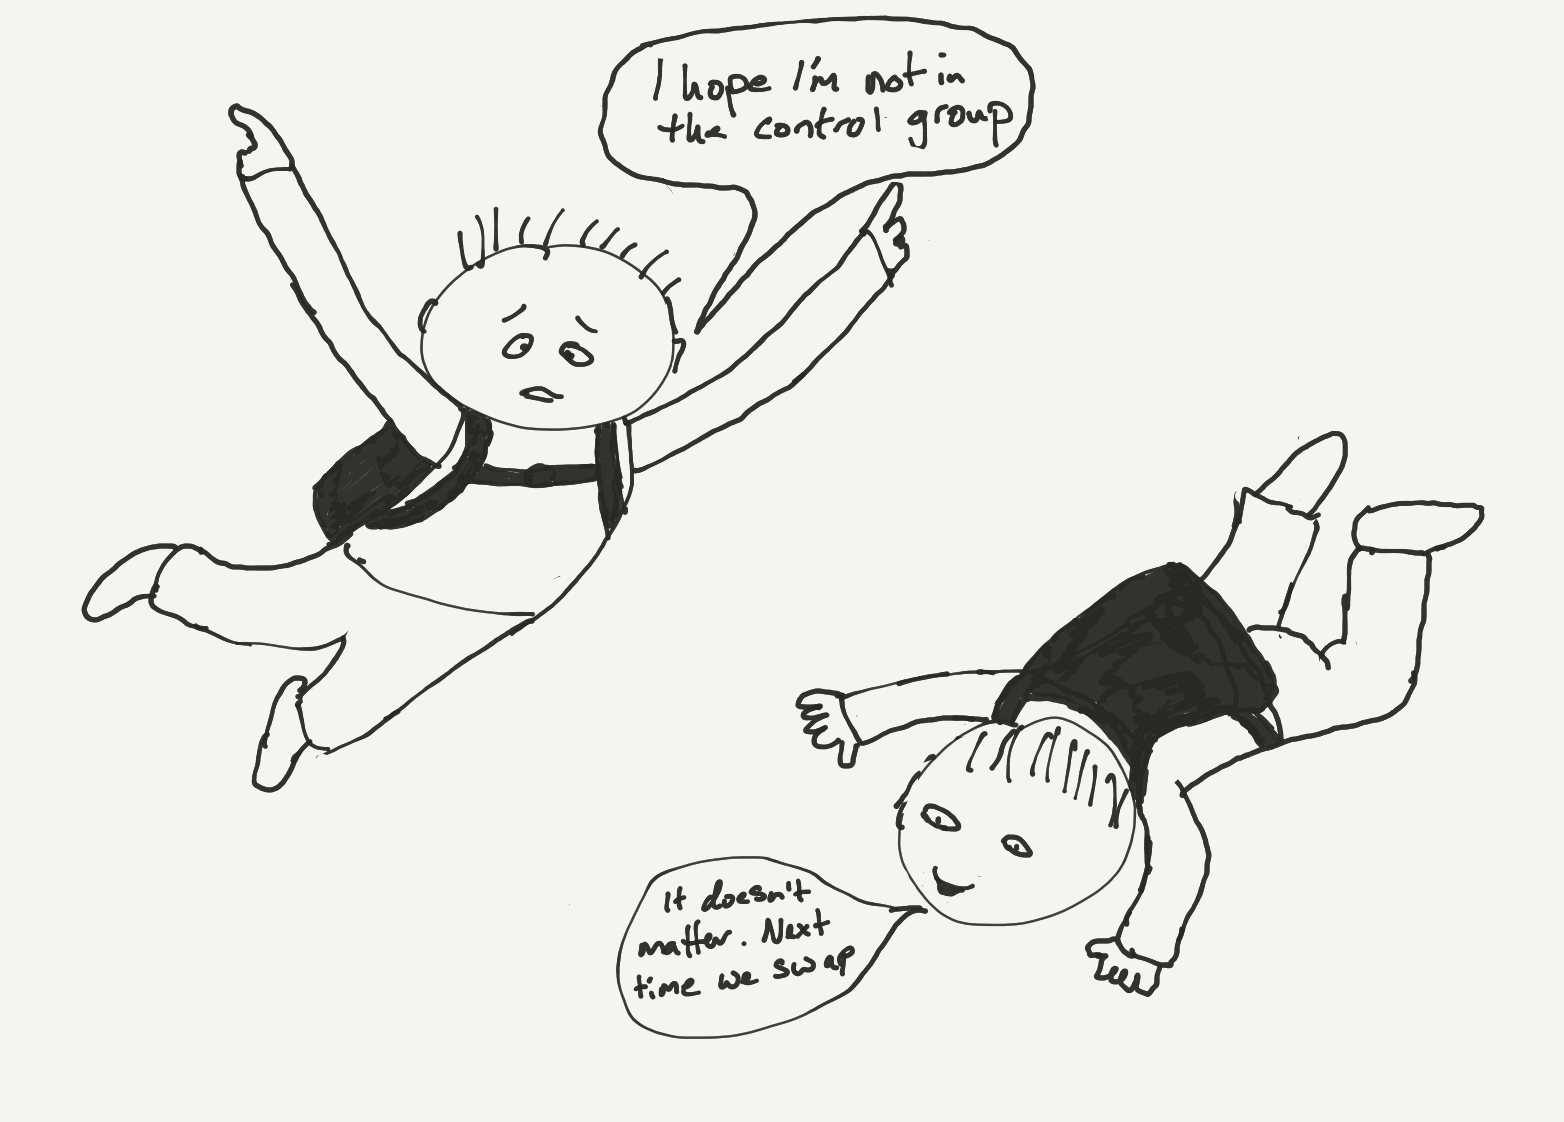
\includegraphics[scale=.4]{double_blind_parashute_trial_cartoon.png}
\end{center}
\end{figure}

\section{Multi armed bandits}
\todo{is there a way in latex to have a command for referring to each type of thing like figure, subsection, etc such that it can be updated programatically?}

Multi-armed bandits were originally introduce by XXXX to address the problem that it is sub-optimal to fix a probability of treatment in advance as we discussed in subsection \ref{subsec:limitations_of_experiment}. The problem can be formally stated as follows:

\paragraph*{Definition} 
In its classic formulation \cite{Robbins1952} the (stochastic) K-armed bandit describes a sequential decision making problem, with $K$ possible actions or arms. Each arm $i$ is associated with a fixed but unknown reward distribution $\nu_i$. In order to obtain regret bounds, some assumptions are required on the distributions $\nu_i$. It sufficient to assume they are sub-Gaussian.  For each time step $t$ upto a horizon $T$ the learner selects an action $I_t \in \set{1...K}$ and receives a reward, $g_{I_t,t}$, sampled i.i.d from $\nu_i$. The goal of the learner is to maximise the total reward they receive. This problem introduces the fundamental exploration-exploitation trade-off. The learner must balance playing arms that have yielded good results previously with exploring arms about which they are uncertain. 

The performance of bandit algorithms is generally described by the (pseudo) regret, $R(T)$. This is the difference between the expected reward obtained by the algorithm and the expected reward of selecting the best action in every time step. 

\subsection{Regret} How do we measure the performance of a bandit algorithm?

%$\simpleregret = \mu^* - \E{\mu_{\hat a^*_T}}.$ 

Expected Regret
\eqn{
R_T(\pi) = \E{max_{i \in [k]} \sum_{t=1}^T{X_{t,i}}} - \E{\sum_{t=1}^T{X_{t,A(t)}}}
}

Pseudo-Regret
\eqn{
R_T(\pi) &= max_{i \in [k]}\E{\sum_{t=1}^T{X_{t,i}}} - \E{\sum_{t=1}^T{X_{t,A(t)}}} \\
&= n\mu_{i^*} - \E{\sum_{t=1}^T{X_{t,A(t)}}}
}

Simple Regret
\eqn{
\mu_{i^*} - \E{\mu_{\hat i^*}}.
}


An algorithm is learning if it obtains regret that is sub-linear in $T$. 

Scholars in the 1940's found this problem so frustrating that they suggested it be dropped over Germany to distract the scientists there from the war effort.\cite{XXX}. 


Another problem that has attracted a lot of recent attention \cite{Bubeck2009,Audibert2010,Gabillon2012,Karnin2013} within the multi-armed bandit framework is \textit{pure exploration} or \textit{best arm identification}. In this setting, the horizon $T$ represents a fixed budget for exploration after which the algorithm outputs a single best arm $i$. The performance of the algorithm is measured by the simple regret; the expected difference between the mean reward of the (truly) optimal arm and the mean reward of the arm selected by the algorithm, $R_s(T) = \mu^* - \E{\mu_i}$ . This problem arises naturally in applications where there is a testing or evaluation phase, during which regret is not incurred, followed by a commercialisation or exploitation phase. For example, many strategies might be assessed via simulation prior to one being selected and deployed. The simple regret for a K-armed bandit is lower bounded by $\bigo{\sqrt{K/T}}$ \cite{Bubeck2009}.

\todo{connect bandit regret to early stopping of experiment problem}
The problem of when to stop an experiment early can also be phrased as a bandit problem and analysed with the same techniques. XXX et al showed that if use an experimental setup with early stopping, the regret you obtain will be at least twice that you could have achieved had you made each decision sequentially using a bandit approach. Of course this neglect any costs that might be associated with the complexity in implementation of the two approaches. 

\subsection{The exploration/exploitation trade-off}
A central aspect to bandit problem is the trade of between exploiting the information we have already obtained with exploring options about which we remain uncertain. Suppose you have sampled five of your local restaurants and found one which you really enjoyed. How often should you eat there versus exploring new options. The degree to which you should explore versus exploit depends on how many step remain to go in the game and what assumptions you make about the distributions from which the rewards are sampled. If this is your last meal you might as well just eat the food you enjoy most but if you hope to live for many meals to come then you stand to gain by sampling a wider range of options. In many cases, the total number of rounds that you will get to play in the game is unknown. If you cannot imagine that it would be possible for a meal to be substantially better than that which you obtain (in expectation) at your current favourite then there is little point exploring further. 

\subsection{Key approaches and results}

The lower bound on the worst case regret for any algorithm (stochastic or adversarial) for the K-armed bandit problem is  $\bigomega{\sqrt{TK}}$ \cite{Auer1995}.

A key algorithm for stochastic bandits, with tractable analysis and strong performance guarantees, is the UCB algorithm \cite{Auer2002}. They key to this algorithm is that it keeps track of an upper confidence bound (hence UCB) on the expected reward for each arm and selects the arm with the highest one. This balances exploration and exploitation as an arm with a high upper confidence bound must have either a high expected reward or large uncertainty on the expected reward. Assume for rotational simplicity that $\mu_1 > \mu_2 > ... > \mu_K$, such that $\mu^* = \mu_1$, and let $\Delta_i = \mu_i - \mu^*$ be the sub-optimal for each arm. The (problem dependent) regret for UCB is bounded by: 

\eqn {
R^{ucb}(T) \in \bigo{\sum_{i=2}^K \frac{1}{\Delta_i}\log(T)}
}

This bound blows up as differences $\Delta_i \rightarrow 0$, however the regret itself does not - since although we may not be able to distinguish arms with very small $\Delta_i$ from the optimal arm, we also do not lose much by selecting them. In the worst case, $R^{ucb}(T) = \bigo{\sqrt{TK\log(T)}}$ \cite{Bubeck2012}. Subtle modifications to the UCB algorithm can eliminate the logarithmic term in this worst case regret bound. This yields $R^{ucb}(T) = \bigo{\sqrt{TK}}$ and closes the gap with the worst case lower bound \cite{Audibert2009,Lattimore2015}, whilst retaining a good problem dependent bound of the form achieved by UCB \cite{Lattimore2015}.


One key principle that has motivated the design of a number \todo{ask Tor are there actually others aside from UCB?} of key bandit algorithms is the idea of \emph{optimism in the face of uncertainty}. An algorithm is trying to simultaneously obtain large rewards and extract as much information as possible. If an action has a high upper bound on the possible reward then either the expected reward must be high or the algorithm must be very uncertain about it. Choosing it should yield either a good reward or useful information. This is the key idea behind the UCB algorithm \citep{xxx}. The remaining complexity lies in optimising how we compute confidence intervals to trade of exploration and exploitation as the game proceeds. Subtle variations in how the confidence intervals are defined lead to a number of algorithms, which are optimised to slightly different settings. SETTINGS NOT QUITE RIGHT WORD. \citep{xxx}.


\subsection{The need to add structure}
The regret for a bandit problem grows linearly with the number of (sub-optimal) actions. This makes problems with large or infinite actions spaces intractable. REFERENCE equation showing linearity with arms. CHECK ITS TRUE. 

The classic multi-armed bandit is a powerful tool for sequential decision making. However, the regret grows linearly with the number of (sub-optimal) actions and many real world problems have large or even infinite action spaces. This has led to the development of a wide range of models that assume some structure across the reward distributions for different arms, for example generalised linear bandits \cite{filippi2010parametric}, dependent bandits \cite{Pandey2007}, X-armed bandits \cite{Bubeck2010} and Gaussian process bandits \cite{srinivas2009gaussian}, or that consider more complex feedback, for example the recent work on graph feedback \cite{Mannor2011,Lelarge2012,Alon2013,Buccapatnam2014,Kocak2014,Alon2015} and partial monitoring \cite{Piccolboni2001,Bartok2014}. 


\subsection{Key related settings}

\subsubsection{Adversarial Bandits}
In the classical multi-armed bandit problem, the rewards for each arm are sampled stochastically from a fixed (but unknown) distribution. There is a large body of work analysing a more general formulation of the bandit problem that relaxes this stochastic assumption. 

Adversarial bandits are an alternate, widely studied, setting that relaxes the assumption that rewards are generated stochastically. Instead, simultaneously with the learner selecting an action $I_t$, a potentially malicious adversary selects the reward vector $\boldsymbol{g}_t$. As in the stochastic setting, the learner then receives reward $g_{I_t,t}$. The seminal algorithm for adversarial bandits is Exp-3, which, like UCB, obtains regret $\bigo{\sqrt{TK\log(T)}}$ regret \cite{Auer1995}. Optimal algorithms, with $R(T) = \bigo{\sqrt{TK}}$, have also been demonstrated for the adversarial setting \cite{Audibert2009}.

\paragraph*{Definition of the Adversarial bandit problem}
\begin{itemize}
\item Different notation of regret
\item Adversarial bandits are not immune to issues of feedback cycles or drift in the reward distribution because a constancy is implicit in the definition of regret. 
\end{itemize}

\subsubsection{Contextual bandits}
In the previous sections each decision was identical. If we were imaging treating patients, we assume that we have no additional information about each patient that is relevant to deciding how to treat them. However, in many key applications such as serving ads, etc, etc. we clearly do have additional information that we wish to take into account. In the contextual bandit setting the goal is to learn 

\eq {
\P{Y|a,x}
} 

As opposed to the standard bandit setting where we are attempting to estimate 

\eq{
\P{Y|a}
}

The formal definition of a contextual bandit problem is

The simplest way to generalise the standard bandit algorithms to the contextual case (where the context is discrete) is to simply have a separate standard bandit instance for each possible setting of the context. Regrettably this approach scales terribly with increasing complexity of the context. \todo{quantify this}. It cannot be applied at all if the context is continuous. 

The approach to solving this problem parallels those from supervised learning and continuous armed bandits. We make assumptions about the smoothness of the problem. Values of context that are similar should lead to comparable rewards for a given action. 

Regret bounds \todo {insert regret bounds for contextual bandits} 

It should be noted that there is an important difference between the approaches we can apply to the contextual bandit versus the supervised learning setting. As for the casual effect estimation problem, we cannot utilise cross-validation offline to select model parameters. This makes contextual bandit algorithms degrade faster than supervised learning ones as we add irrelevant variables. \todo{ask Tor if he thinks this is correct}

RUN A SIMULATION COMPARING HOW supervised learning and contextual bandits degrade as we add more features. What would be a fair comparison?

\subsubsection{Markov decision processes}
In the bandit setting the reward distributions for each arm are assumed to be fixed. A much studied generalisation is the Markov decision process or MDP. In an MDP we assume there the environment has some state. The reward an agent receives depends on the state of the environment and the action the agent selects. The environment then evolves stochastically depending on the agents action. Multi-armed bandits can be considered a single state MDP, where no matter what action the agent selects, the environment returns to that state. 

Insert a graphical representation of an MDP

What assumptions are required to make MDPs tractable. 

What is the basic algorithm (Q-learning)

What are the key results.

\subsubsection{Dynamic Systems}
\begin{itemize}
\item An explicit model of actions in a partially known system (eg HMM)
\item Feynman-Kac Lemma; Solving a PDE can be converted to a stochastic process
\end{itemize}


\chapter{Causal Bandits: Unifying the approaches}

\section{The framework}
A natural way to connect the causal framework with the bandit setting is to model the action space as interventions on variables in a causal directed acyclic graph. Each possible assignment of variables to values is a potential action (or bandit arm), see figure \ref{} for a simple example. In some settings, it makes sense to restrict the action space available to the agent to a subset of all the possible actions, for example only the set of single variable interventions. The reward could be a general function of the action selected and the final state of the graph. However for simplicity, we will consider the reward to be the value of a single specified node minus the cost of the selected action. In this thesis I examine the case where the causal graph is known. We refer to these problems as \emph{causal bandit problems}.  Extending this work to simultaneously learning the casual graph is discussed in section \ref{XXX}.

\subsubsection{Definition of casual bandit problem} \todo{make proper definition}
A learner for a casual bandit problem is given the casual model's graph $\mathcal{G}$ and a set of \emph{allowed actions} $\mathcal{A}$.
One variable $Y \in \mathcal{X}$ is designated as the \emph{reward variable} and takes on values in $\{0, 1\}$.


\begin{figure}[h]
\caption{A simple causal graphical model and corresponding complete action space. A and B represent binary variables that can be intervened on and Y represents the reward.}
\label{fig:unify_frameworks}
\centering
\begin{subfigure}[c]{0.3\textwidth}
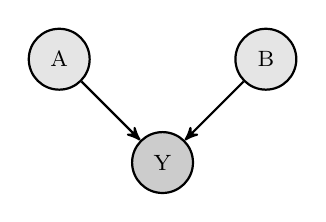
\begin{tikzpicture}[->,shorten >=0pt,shorten <=0pt,node distance=3em,thick,main node/.style={observed}, tg/.style={target}]
\node[main node](1){A};
\node[tg, below right=of 1](2){Y};
\node[main node, above right=of 2](3){B};
\path[]
	(1) edge (2)
	(3) edge (2);
\end{tikzpicture}
\end{subfigure}
\begin{subfigure}[t]{0.4\textwidth}
Actions = \begin{tabular}{|c|}
	\hline
  do(A=0,B=0) \\
  do(A=0,B=1) \\
  do(A=1,B=0) \\
  do(A=1,B=1) \\
  \hline
  do(A=0) \\
  do(A=1) \\
  do(B=0) \\
  do(B=1) \\
  do() \\
  \hline
\end{tabular}
\end{subfigure}
\end{figure} 

The number of actions or arms grows exponentially with the number of variables in the graph,
making it important to use algorithms that leverage the graph structure to reduce the
search space. Modelling a problem as a causal graph only makes sense when rewards are generated stochastically - since causal graphs fundamentally model probability distributions over variables. Thus the connection is to stochastic bandit problems (although adversarial bandits algorithms may be applied to stochastic problems).

We now need to specify the feedback model for the causal bandit problem. What information is available to the decision making agent before and after they select an action? The causal bandit problem takes on characteristics of different bandit settings depending on the assumptions we make about what actions are available to the agent, what variables are observed and whether they are observed before or after the action is chosen. 

Enumerate the settings
\begin{enumerate}
\item Bandit feedback: the agent selects an action and then observes only the reward of that action. If feedback is received only on the reward node then the do-calculus can be applied to eliminate some actions immediately, before any experiments are performed and then a standard bandit algorithm can be run on the remaining actions. See figure XXX as an example. 
\item Bandit feedback with side information (context). The agent can view the value of some variables prior to selecting an action. After selecting they observe the reward of the selected node. 
\item Post action feedback:
\end{enumerate}

If we receive feedback on additional nodes, the problem can be more interesting. In addition to being able to eliminate some actions prior to sampling any data as in the previous case, taking one action may give us some information on actions that were not selected. Consider again the model in figure \ref{fig:unify_frameworks}. The causal structure implies: 

\eqn {
P(Y|do(A = 0)) &= P(Y|do(),A = 0) \\
&= P(Y|do(B=0),A=0)P(B=0)+P(Y|do(B=1),A=0)P(B=1) 
}

Thus we gain information about the reward for the action $do(A=0)$ from selecting the action $do()$ or $do(B = b)$ and then observing $A = 0$.  

We only get this form of side information for actions that don't specify the value of every variable, ie those in the bottom half of the table in figure \ref{fig:unify_frameworks}. Since the reward distribution for actions that set a subset of the variables is the result of marginalising out other variables, they can only be optimal if they have lower cost. So if the cost of all actions is constant (no matter how many variables must be set), then the problem has the same characteristics as if only the reward node were observable.

If the information on the value of additional nodes is available prior to selecting an action the problem resembles a contextual bandit. For example if we observe $A = 0$ then, in deciding between the actions $do(B=0)$ and $do(B=1)$, we would want information on $P(Y|A=0,B=0)$ and $P(Y|A=0,B=1)$.  Note, side information can still arise if we learn the value of some variables prior to selecting an action and some afterwards. 

Although we will focus on the intervene-then-observe ordering of events within each round, other scenarios are possible. If the non-intervened variables are observed before an intervention is selected our framework reduces to stochastic contextual bandits, which are already reasonably well understood~\citep{Agarwal2014}. Even if no observations are made during the rounds, the causal model may still allow offline pruning of the set of allowable interventions thereby reducing the complexity.


\section{Related work}
\begin{enumerate}
\item leaning from log data
\item bandits with imperfect compliance
\item rigged casino paper
\end{enumerate}

\begin{figure}[h]
\caption{Example causal graph (based on \cite{Koller2009}) where the outcome of interest (reward) is cholesterol level . The do-calculus can be applied to eliminate some actions immediately without the need to do any experiments. For example, no actions involving 'Test Result' need to be considered and interventions on 'Diet' do not need to be considered in conjunction with any other variables.}
\label{fig:cholesterol_graph}
\centering
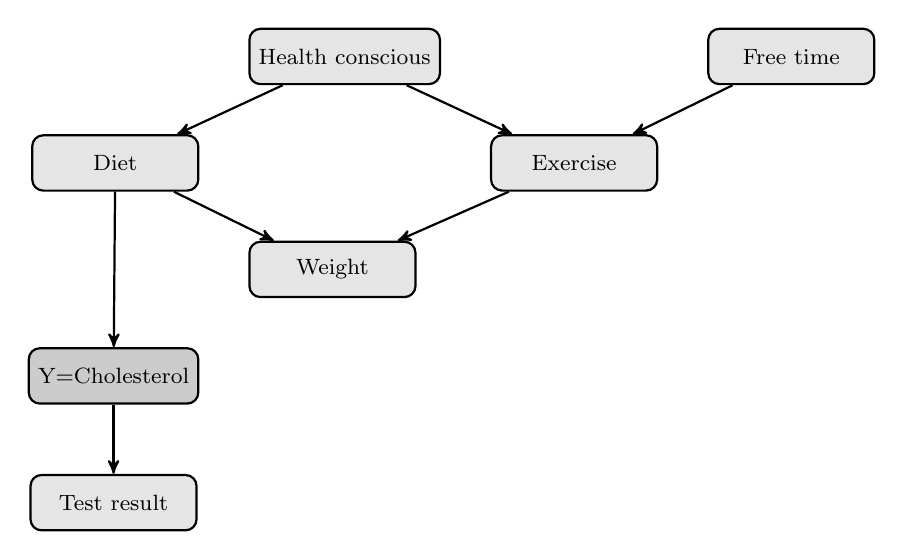
\begin{tikzpicture}[->,shorten >=0pt,shorten <=0pt,node distance=2.5em,thick,node/.style={observedrect},tg/.style={targetrect}]
\node[node](1){Health conscious};
\node[node, below left=of 1](2){Diet};
\node[node, below right=of 1](3){Exercise};
\node[node, below right=of 2](4){Weight};
\node[tg,below left=of 4](5){Y=Cholesterol};
\node[node, below =of 5](6){Test result};
\node[node, above right=of 3](7){Free time};
\path[]
	(1) edge (2) edge (3)
	(2) edge (4) edge (5)
	(3) edge (4)
	(5) edge (6)
	(7) edge (3);
\end{tikzpicture}
\end{figure}


\section{Causal bandits with post action feedback}
WHY THIS PROBLEM. This work was presented at NIPS 2016 \ref{}.
\todo{add relevant stuff from introduction section}

\subsection{Notation}

We will assume each variable only takes on a finite number of distinct values. (The path to relaxing this assumption would be through levering the work on continuous armed bandits). 

The \emph{parents} of a variable $X_i$, denoted $\parents{X_i}$, is the set of all variables $X_j$ such that there is an edge from $X_j$ to $X_i$ in $\mathcal{G}$.

An \emph{intervention or action (of size $n$)}, denoted $do(\vec{X}=\vec{x})$, assigns the values $\vec{x}=\{x_1, \ldots, x_n\}$ to the corresponding variables $\vec{X}=\{X_1, \ldots, X_n\} \subset \mathcal{X}$ with the empty intervention (where no variable is set) denoted $do()$.


We denote the expected reward for the action $a = do(\vec{X} = \vec{x})$ by $\mu_{a} := \E{Y | do(\vec{X} = \vec{x})}$ and 
the optimal expected reward by $\mu^* := \max_{a\in\actions} \mu_{a}$. 


\subsection{Definition of causal bandit game with post-action feedback}
\todo{ re-read and incorporate response from reviewer feedback for NIPS}

The causal bandit game proceeds over $T$ rounds.
In round $t$, the learner \emph{intervenes} by choosing $a_t = do(\vec{X}_t = \vec{x}_t) \in \mathcal{A}$ based on previous observations. 
It then \emph{observes} sampled values for all non-intervened variables $\vec{X}^c_t$ drawn from $\P{\vec{X}^c_t | do(\vec{X}_t = \vec{x}_t)}$, 
including the \emph{reward} $Y_t \in \{0,1\}$. 
After $T$ observations the learner outputs an estimate of the optimal action $\hat a^*_T \in \actions$ based on its prior observations.

The objective of the learner is to minimise the simple regret $\simpleregret = \mu^* - \E{\mu_{\hat a^*_T}}.$ This is sometimes refereed to as a ``pure exploration''~\citep{Bubeck2009a} or ``best-arm identification'' problem~\citep{Gabillon2012a} and is most appropriate when, as in drug and policy testing, the learner has a fixed experimental budget after which its policy will be fixed indefinitely. 

We note that classical $K$-armed stochastic bandit problem can be recovered in our framework by considering a simple causal model with one edge connecting a single variable $X$ that can take on $K$ values to a reward variable $Y \in \set{0,1}$ where $\P{Y = 1|X} = r(X)$ for some arbitrary but unknown, real-valued function $r$. The set of allowed actions in this case is $\mathcal{A} = \{ do(X = k) \colon k \in \{1, \ldots, K\}\}$. Conversely, any causal bandit problem can be reduced to a classical stochastic $|\mathcal{A}|$-armed bandit problem by treating each possible intervention as an independent arm and ignoring all sampled values for the observed variables except for the reward. Intuitively though, one would expect to perform better by making use of the extra structure and observations.


\subsection{The parallel bandit problem}

In this section we propose and analyse an algorithm for achieving the optimal regret in a natural special case of the causal bandit problem which we call the {\it parallel bandit}.
It is simple enough to admit a thorough analysis but rich enough to model the type of problem discussed in \ref{XXX}, including the farming example. It also suffices to witness the regret gap between algorithms that make use of causal models and those which do not.

The causal model for this class of problems has $N$ binary variables $\{ X_1, \ldots, X_N \}$ where each $X_i \in \{0,1\}$ are independent causes of a reward variable $Y \in \set{0,1}$, as shown in Figure~\ref{fig:parallel}. All variables are observable and the set of allowable actions are all size 0 and size 1 interventions: $\mathcal{A} = \set{do()} \cup \set{ do(X_i = j) \colon 1 \leq i \leq N \text{ and } j \in \set{0,1}}$

In the farming example from the introduction, $X_1$ might represent temperature (\eg, $X_1=0$ for low and $X_1=1$ for high). The interventions $do(X_1 = 0)$ and $do(X_1 = 1)$ indicate the use of shades or heat lamps to keep the temperature low or high, respectively.

\begin{figure}
    \begin{subfigure}[b]{0.34\textwidth}
	\centering    
          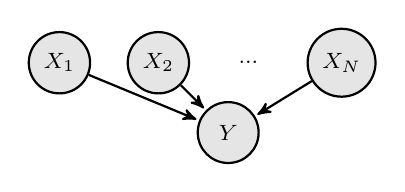
\begin{tikzpicture}[->,>=stealth',shorten >=1pt,auto,node distance=.45cm,
  thick,main node/.style={observed}, hidden/.style={empty},background rectangle/.style={fill=olive!45}]
%every node/.style={scale=0.6}
 %nodes
\node[main node](1){$X_{1}$};
\node[main node, right=of 1](2){$X_{2}$};
\node[hidden, right=of 2](3){$...$};
\node[main node, right=of 3](4){$X_{N}$};
\node[main node, below right=of 2](5){$Y$};
 \path[every node/.style={font=\tiny}]
    (1) edge (5)
    	(2) edge (5)
    (4) edge (5);
\end{tikzpicture}
        \caption{Parallel graph}
        \label{fig:parallel}
    \end{subfigure}
    \begin{subfigure}[b]{0.2\textwidth}
    \centering
        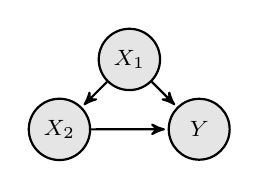
\begin{tikzpicture}[->,>=stealth',shorten >=1pt,auto,node distance=.45cm,
  thick,main node/.style={observed}, hidden/.style={empty},background rectangle/.style={fill=olive!45}]
\node[main node](1){$X_1$};
\node[main node, below left=of 1](2){$X_2$};
\node[main node, below right=of 1](4){$Y$};
 \path[every node/.style={font=\tiny}]
    (1) edge (2)
    (1) edge (4)
    (2) edge (4);
\end{tikzpicture}
        \caption{Confounded graph}
        \label{fig:causalStructure_confounded}
    \end{subfigure}
    \begin{subfigure}[b]{0.4\textwidth}
    \centering
         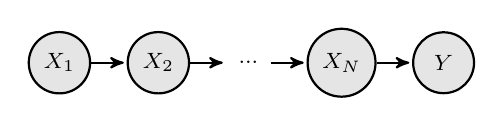
\begin{tikzpicture}[->,>=stealth',shorten >=1pt,auto,node distance=.45cm,
  thick,main node/.style={observed}, hidden/.style={empty},background rectangle/.style={fill=olive!45}]
\node[main node](1){$X_{1}$};
\node[main node, right=of 1](2){$X_{2}$};
\node[hidden, right=of 2](3){$...$};
\node[main node, right=of 3](4){$X_{N}$};
\node[main node, right=of 4](5){$Y$};
 \path[every node/.style={font=\tiny}]
    (1) edge (2)
  	(2) edge (3)
    (3) edge (4)
    (4) edge (5);
\end{tikzpicture}
        \caption{Chain graph}
        \label{fig:causalchain}
    \end{subfigure}
    \caption{Causal Models}\label{fig:causalmodels}
    \vspace{-.5cm}
\end{figure}


In each round the learner either purely observes by selecting $do()$ or sets the value of a single variable. The remaining variables are simultaneously set by independently biased coin flips. The value of all variables are then used to determine the distribution of rewards for that round. Formally, when not intervened upon we assume that each $X_i \sim \bernoulli(q_i)$ where $\vec{q} = (q_1, \ldots, q_N) \in [0,1]^N$ so that $q_i = \P{X_i = 1}$.

The value of the reward variable is distributed as $\P{Y = 1|\vec{X}} = r(\vec{X})$ where 
$r : \{0,1\}^N \to [0,1]$ is an arbitrary, fixed, and unknown function. 
In the farming example, this choice of $Y$ models the success or failure of a seasons crop, 
which depends stochastically on the various environment variables.


\paragraph{The Parallel Bandit Algorithm}
%\label{sub:par-bandit-alg}
The algorithm operates as follows. For the first $T/2$ rounds it chooses $do()$ to collect observational data. As the only link from each $X_1,\ldots,X_N$ to $Y$ is a direct, causal one, $\P{Y|do(X_i=j)}=\P{Y|X_i=j}$. Thus we can create good estimators for the returns of the actions $do(X_i = j)$ for which $\P{X_i = j}$ is large. The actions for which $\P{X_i = j}$ is small may not be observed (often) so  estimates of their returns could be poor. To address this, the remaining $T/2$ rounds are evenly split to estimate the rewards for these infrequently observed actions. The difficulty of the problem depends on $\vec{q}$ and, in particular, how many of the variables are unbalanced (\ie, small $q_i$ or $(1-q_i)$). For $\tau \in [2...N]$ let $I_\tau = \set{ i : \min\set{q_i, 1-q_i} < \frac{1}{\tau}}$. Define

\eq{
\label{eq:m-simple}
m(\vec{q}) = \min \set{ \tau : |I_{\tau}| \leq \tau}\,.
}


\begin{algorithm}[H]
\caption{Parallel Bandit Algorithm}\label{alg:simple}
\begin{algorithmic}[1]
\STATE {\bf Input:} Total rounds $T$ and $N$.
\FOR{$t \in 1,\ldots,T / 2$}
\STATE Perform empty intervention $do()$
\STATE Observe $\vec{X}_t$ and $Y_t$
\ENDFOR
\FOR{$a = do(X_i = x) \in \actions$}
\STATE Count times $X_i = x$ seen: $T_a = \sum_{t=1}^{T/2} \ind{X_{t,i} = x}$
\STATE Estimate reward: $\hat{\mu}_a = \frac{1}{T_a} \sum_{t=1}^{T/2} \ind{X_{t,i} = x} Y_t$ \\[0.2cm]
\STATE Estimate probabilities: $\hat{p}_a = \frac{2 T_a}{T}$,\,\, $\hat q_i = \hat p_{do(X_i = 1)}$
\ENDFOR
\STATE Compute $\hat{m} = m(\vec{\hat q})$ and $A = \set{a \in \actions \colon \hat{p}_a \leq \frac{1}{\hat m}}$.
\STATE Let $T_A := \frac{T}{2 |A|}$ be times to sample each $a\in A$.
\FOR{$a = do(X_i = x) \in A$}
\FOR{$t \in 1,\ldots,T_A$}
\STATE Intervene with $a$ and observe $Y_t$
\ENDFOR
\STATE Re-estimate $\hat{\mu}_a = \frac{1}{T_A} \sum_{t=1}^{T_A} Y_t$
\ENDFOR
\RETURN estimated optimal $\hat{a}^*_T \in \argmax_{a\in\actions} \hat{\mu}_a$
\end{algorithmic}
\end{algorithm}

$I_\tau$ is the set of variables considered unbalanced and we tune $\tau$ to trade off identifying the low probability actions against not having too many of them, so as to minimise the worst-case simple regret. When $\vec{q} = (\frac{1}{2}, \ldots, \frac{1}{2})$ we have $m(\vec{q}) = 2$ and when $\vec{q} = (0, \ldots, 0)$ we have $m(\vec{q}) = N$. We do not assume that $\vec{q}$ is known, thus Algorithm \ref{alg:simple} also utilises the samples captured during the observational phase to estimate $m(\vec{q})$. Although very simple, the following two theorems show that this algorithm is effectively optimal.


\begin{theorem}\label{thm:uq-simple}
Algorithm \ref{alg:simple} satisfies
\eq{
\simpleregret \in \bigo{\sqrt{\frac{m(\vec{q})}{T}\log\left(\frac{NT}{m(\vec{q})}\right)}}\,.
}
\end{theorem}


\begin{theorem}\label{thm:lower}
For all strategies and $T$, $\vec{q}$, there exist rewards such that
$\displaystyle \simpleregret 
\in \Omega\left(\sqrt{\frac{m(\vec{q})}{T}}\right)$.
\end{theorem}


The proofs of Theorems \ref{thm:uq-simple} and \ref{thm:lower} may be found in Sections \ref{sec:thm:uq-simple} and \ref{sec:thm:lower} respectively.

The proofs of Theorems \ref{thm:uq-simple} and \ref{thm:lower} follow by carefully analysing the concentration
of $\hat p_a$ and $\hat m$ about their true values and may be found in the supplementary material.

%We prove a lower bound on the simple regret that matches up to logarithmic factors the upper bound given in Theorem \ref{thm:uq-simple}. 
By utilising knowledge of the causal structure, Algorithm \ref{alg:simple} effectively only has to explore the $m(\vec{q})$ 'difficult' actions. Standard multi-armed bandit algorithms must explore all $2N$ actions and thus achieve regret  $\smash{\Omega(\sqrt{N/T})}$. Since $m$ is typically much smaller than $N$, the new algorithm can significantly outperform classical bandit algorithms in this setting. In practice, you would combine the data from both phases to estimate rewards for the low probability actions. We do not do so here as it slightly complicates the proofs and does not improve the worst case regret.

\subsection{General graphs}
We now consider the more general problem where the graph structure is known, but arbitrary. For general graphs, $\P{Y|X_i=j} \neq \P{Y|do(X_i=j)}$ (correlation is not causation). However, if all the variables are observable, any causal distribution $\P{X_1...X_N|do(X_i=j)}$ can be expressed in terms of observational distributions via the truncated factorisation formula \citep{Pearl2000}. 
\eq{
\P{X_1...X_N|do(X_i=j)} = 
\prod_{k \neq i}\P{X_k|\parents{X_k}}\delta(X_i - j)\,, 
} 
where $\parents{X_k}$ denotes the parents of $X_k$ and $\delta$ is the Dirac delta function. 

We could naively generalize our approach for parallel bandits by observing for $T/2$ rounds, applying the truncated product factorisation to 
write an expression for each $\P{Y|a}$ in terms of observational quantities and explicitly playing the actions for which the observational 
estimates were poor. However, it is no longer optimal to ignore the information we can learn about the reward for intervening on one variable 
from rounds in which we act on a different variable. Consider the graph in Figure \ref{fig:causalchain} and suppose each variable deterministically 
takes the value of its parent, $X_k = X_{k-1}$ for $k\in {2,\ldots,N}$ and $\P{X_1} = 0$. We can learn the reward for all the interventions $do(X_i = 1)$ 
simultaneously by selecting $do(X_1 = 1)$, but not from $do()$. In addition, variance of the observational estimator for $a = do(X_i = j)$ can be 
high even if $\P{X_i = j}$ is large. Given the causal graph in Figure \ref{fig:causalStructure_confounded}, $\P{Y|do(X_2= j)} = \sum_{X_1}\P{X_1}\P{Y|X_1, X_2 = j}$. 
Suppose $X_2 = X_1$ deterministically, no matter how large $\P{X_2 = 1}$ is we will never observe $(X_2=1,X_1 = 0)$ and so cannot 
get a good estimate for $\P{Y|do(X_2=1)}$. 

To solve the general problem we need an estimator for each action that incorporates information obtained from every other action and a way to optimally 
allocate samples to actions. To address this difficult problem, we assume the conditional interventional distributions $\P{\parents{Y}|a}$ (but not $\P{Y|a}$) 
are known. These could be estimated from experimental data on the same covariates but where the outcome of interest differed, such that $Y$ was not included, 
or similarly from observational data subject to identifiability constraints. Of course this is a somewhat limiting assumption, but seems like a natural place to
start. The challenge of estimating the conditional distributions for all variables in an optimal way is left as an interesting future direction.
Let $\eta$ be a distribution on available interventions $a \in \calA$ so $\eta_a \geq 0$ and $\sum_{a \in \calA} \eta_a = 1$. 
Define $Q = \sum_{a \in \calA} \eta_a \P{\parents{Y}|a}$ to be the mixture distribution over the interventions with respect to $\eta$.



\begin{algorithm}[H]
\caption{General Algorithm}\label{alg:general}
\begin{algorithmic}
\STATE {\bf Input:} $T$, $\eta \in [0,1]^{\calA}$, $B \in [0,\infty)^{\calA}$
\FOR{$t \in \set{1,\ldots,T}$}
\STATE Sample action $a_t$ from $\eta$
\STATE Do action $a_t$ and observe $X_t$ and $Y_t$
\ENDFOR
\FOR{$a \in \calA$}
\STATE
\eq {
\hat \mu_a =  \frac{1}{T} \sum_{t=1}^T Y_t R_a(X_t)  \ind{R_a(X_t) \leq B_a}
}
\ENDFOR
\STATE {\bf return} $\hat a^*_T = \argmax_a \hat \mu_a$
\end{algorithmic}
\end{algorithm}


Our algorithm samples $T$ actions from $\eta$ and uses them to estimate the returns $\mu_a$ for all $a \in \calA$ simultaneously via a truncated importance weighted estimator. Let $\parents{Y}(X)$ denote the realisation of the variables in $X$ that are parents of Y and define $R_a(X) = \frac{\Pn{a}{\parents{Y}(X)}}{\Q{\parents{Y}(X)}}$

\eq {
\hat \mu_a =  \frac{1}{T} \sum_{t=1}^T Y_t R_a(X_t)  \ind{R_a(X_t) \leq B_a}\,, 
} 

where $ B_a \geq 0$  is a constant that tunes the level of truncation to be chosen subsequently. The truncation introduces a bias in the estimator, but simultaneously chops the potentially heavy tail that is so detrimental to its concentration guarantees. 

The distribution over actions, $\eta$ plays the role of allocating samples to actions and is optimised to minimise the worst-case simple regret. Abusing notation we define $m(\eta)$ by
\eq{
m(\eta) = \max_{a \in \calA} \EEa\left[\frac{\Pn{a}{\parents{Y}(X)}}{\Q{\parents{Y}(X)}}\right]\,,\text{ where } \EEa \text{ is the expectation with respect to } \Pn{a}.
}

We will show shortly that $m(\eta)$ is a measure of the difficulty of the problem that approximately coincides with the version for parallel bandits, justifying the name overloading.

\begin{theorem}\label{thm:general}
If Algorithm \ref{alg:general} is run with $B \in \R^{\calA}$ given by $B_a = \sqrt{\frac{m(\eta)T}{\log\left(2T|\calA|\right)}}\,.$

\eq{
\simpleregret \in \bigo{\sqrt{\frac{m(\eta)}{T} \log\left(2T|\calA|\right)}}\,.
}
\end{theorem}

The proof is in Section \ref{sec:thm:general}.

Note the regret has the same form as that obtained for Algorithm \ref{alg:simple}, with $m(\eta)$ replacing $m(q)$. Algorithm \ref{alg:simple} assumes only the graph structure and not knowledge of the conditional distributions on $X$. Thus it has broader applicability to the parallel graph than the generic algorithm given here. We believe that Algorithm \ref{alg:general} with the optimal choice of $\eta$ is close to minimax optimal, but leave lower bounds
for future work.


\paragraph{Choosing the Sampling Distribution} Algorithm \ref{alg:general} depends on a choice of sampling distribution $\operatorname{Q}$ that is determined by $\eta$. In light of Theorem \ref{thm:general}
a natural choice of $\eta$ is the minimiser of $m(\eta)$.
\eq{
\eta^* 
= \argmin_\eta m(\eta) = \argmin_\eta \underbrace{\max_{a \in \calA} \EEa \left[\frac{\Pn{a}{\parents{Y}(X)}}{\sum_{b \in \calA} \eta_b \Pn{b}{\parents{Y}(X)}}\right]}_{m(\eta)}\,.
}
Since the mixture of convex functions is convex and the maximum of a set of convex functions is convex, we see that $m(\eta)$ is convex (in $\eta$).
Therefore the minimisation problem may be tackled using standard techniques from convex optimisation. The quantity $m(\eta^*)$ may be interpreted as the minimum achievable worst-case variance of the importance weighted estimator. In the experimental section we present some special cases, but for now we give two simple results. The first shows that $|\calA|$ serves as an upper bound on $m(\eta^*)$.

\begin{proposition}\label{pro:m-bound}
$m(\eta^*) \leq |\calA|$. \textit{Proof.} 
\textup{By definition, $m(\eta^*) \leq m(\eta)$ for all $\eta$. Let $\eta_a = 1/|\calA|\,\forall a$.}
\eq{
m(\eta) 
= \max_a \EEa\left[\frac{\Pn{a}{\parents{Y}(X)}}{\Q{\parents{Y}(X)}}\right] 
\leq \max_a \EEa\left[\frac{\Pn{a}{\parents{Y}(X)}}{\eta_a \Pn{a}{\parents{Y}(X)}}\right] 
= \max_a \EEa\left[\frac{1}{\eta_a}\right] = |\calA| %\qedhere
}
\end{proposition} 

The second observation is that, in the parallel bandit setting, $m(\eta^*) \leq 2m(\boldsymbol{q})$. This is easy to see by letting $\eta_a = 1/2$ for $a = do()$ and $\eta_a = \ind{\P{X_i = j} \leq 1/m(\boldsymbol{q})} / 2m(\boldsymbol{q})$ for the actions corresponding to $do(X_i=j)$, and applying an argument like that for Proposition~\ref{pro:m-bound}. 
The proof is in section XXX.

\begin{remark}\label{rem:truncate}
The choice of $B_a$ given in Theorem \ref{thm:general} is not the only possibility. As we shall see in the experiments, it is 
often possible to choose $B_a$ significantly
larger when there is no heavy tail and this can drastically improve performance by eliminating the bias. This is especially true when the ratio $R_a$ is never too large
and Bernstein's inequality could be used directly without the truncation. For another discussion see the article by \citet{BJQ13} who also use importance weighted estimators
to learn from observational data.
\end{remark}


\subsection{Experiments}
We compare Algorithms \ref{alg:simple} and \ref{alg:general} with the Successive Reject algorithm of \cite{audibert2010best}, Thompson Sampling and UCB under a variety of conditions. Thomson sampling and UCB are optimised to minimise cumulative regret. We apply them in the fixed horizon, best arm identification setting by running them upto horizon $T$ and then selecting the arm with the highest empirical mean. The importance weighted estimator used by Algorithm \ref{alg:general} is not truncated, which is justified in this setting by Remark \ref{rem:truncate}. 

Throughout we use a model in which $Y$ depends only on a single variable $X_1$ (this is unknown to the algorithms). $Y_t \sim \bernoulli(\frac{1}{2}+\epsilon)$ if $X_1=1$ and $Y_t \sim \bernoulli(\frac{1}{2}-\epsilon')$ otherwise, where $\epsilon' = q_1\epsilon/(1-q_1)$. This leads to an expected reward of $\frac{1}{2}+\epsilon$ for $do(X_1=1)$, $\frac{1}{2}-\epsilon'$ for $do(X_1=0)$ and $\frac{1}{2}$ for all other actions. We set $q_i = 0$ for $i \leq m$ and $\frac{1}{2}$ otherwise. Note that changing $m$ and thus $\boldsymbol{q}$ has no effect on the reward distribution. For each experiment, we show the average regret over 10,000 simulations with error bars displaying three standard errors. The code is available from \url{<https://github.com/finnhacks42/causal_bandits>} 

In Figure \ref{fig:simple_vs_m} we fix the number of variables $N$ and the horizon $T$ and compare the performance of the algorithms as $m$ increases. The regret for the Successive Reject algorithm is constant as it depends only on the reward distribution and has no knowledge of the causal structure. For the causal algorithms it increases approximately with $\sqrt{m}$. As $m$ approaches $N$, the gain the causal algorithms obtain from knowledge of the structure is outweighed by fact they do not leverage the observed rewards to focus sampling effort on actions with high pay-offs.


\begin{figure}[h]
    \begin{subfigure}[t]{0.3\textwidth}
		\centering    
    		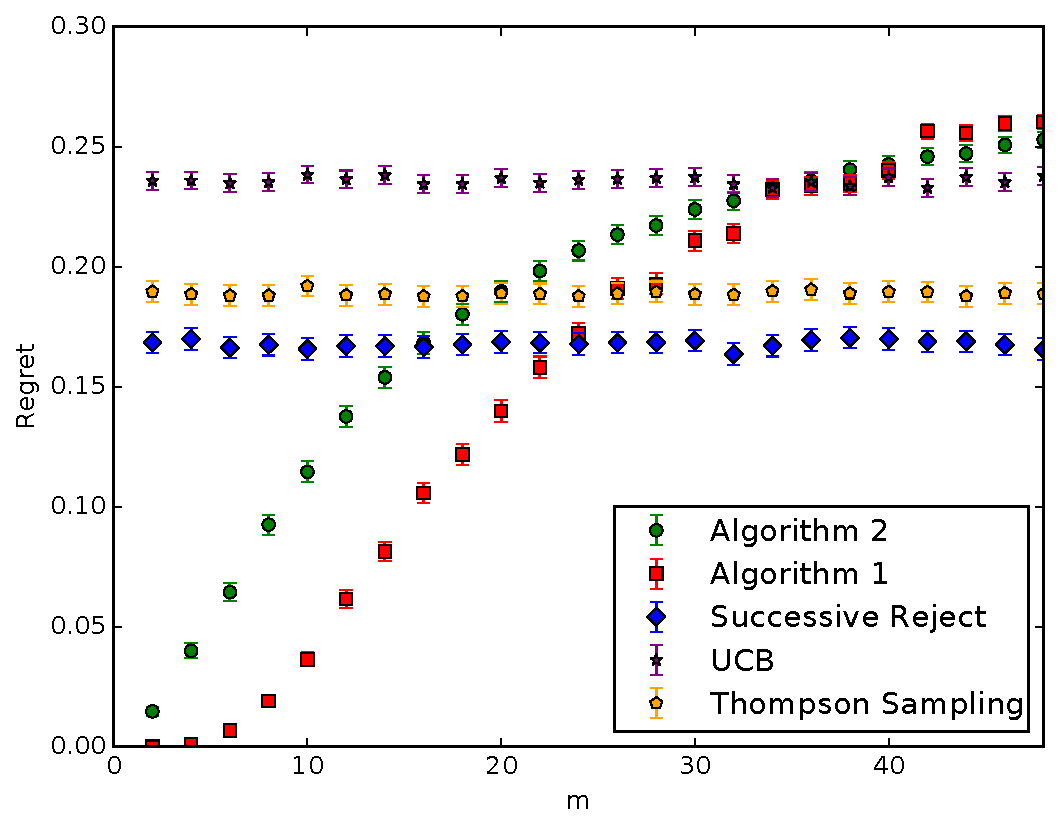
\includegraphics[width=\textwidth]{experiment1_20161020_1247.pdf}
    		\caption{Simple regret vs $m(\boldsymbol{q})$ for fixed horizon $T=400$ and number of variables $N = 50$}
        \label{fig:simple_vs_m}
    \end{subfigure}\hfill
    \begin{subfigure}[t]{0.3\textwidth}
    		\centering
        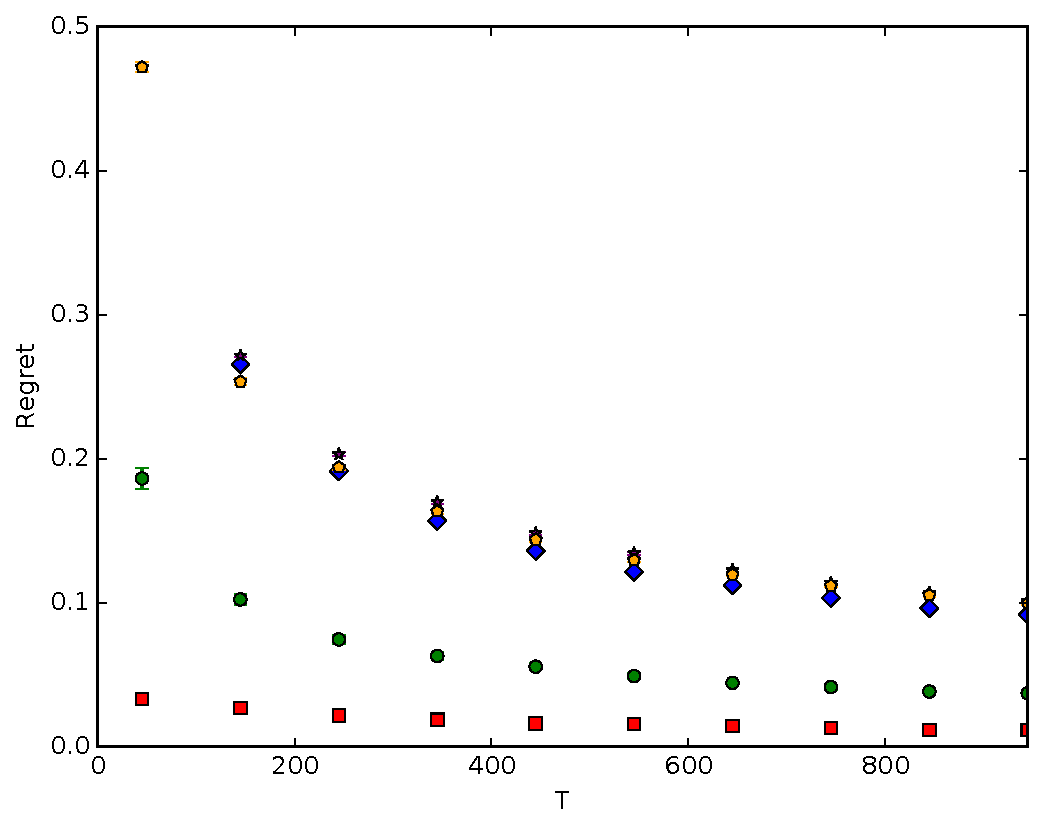
\includegraphics[width=\textwidth]{experiment2_20161020_1249.pdf}
    		\caption{Simple regret vs horizon, $T$, with $N = 50$, $m=2$ and $\epsilon = \sqrt{\frac{N}{8T}}$}
        \label{fig:simple_vs_T_vary_epsilon}
    \end{subfigure}\hfill
    \begin{subfigure}[t]{0.3\textwidth}
    		\centering
    		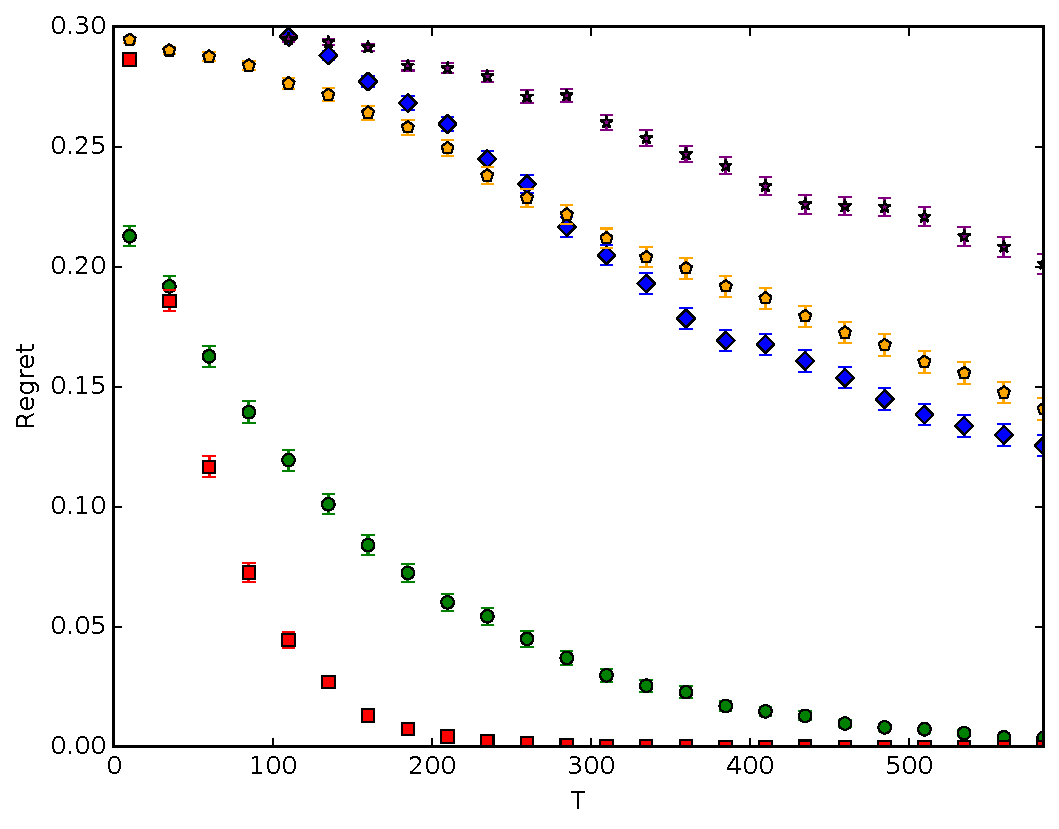
\includegraphics[width=\textwidth]{experiment3_20161020_1252.pdf}
    		\caption{Simple regret vs horizon, $T$, with $N = 50$, $m=2$ and fixed $\epsilon = .3$}
    		\label{fig:simple_vs_T}
    \end{subfigure}
    \caption{Experimental results}
    \label{fig:experiments}
\end{figure}

Figure \ref{fig:simple_vs_T_vary_epsilon} demonstrates the performance of the algorithms in the worst case environment for standard bandits, where the gap between the optimal and sub-optimal arms, $\smash{\epsilon = \sqrt{N/(8T)}}$ , is just too small to be learned. This gap is learn-able by the causal algorithms, for which the worst case $\epsilon$ depends on $m \ll N$. In Figure \ref{fig:simple_vs_T} we fix $N$ and $\epsilon$ and observe that, for sufficiently large $T$, the regret decays exponentially. The decay constant is larger for the causal algorithms as they have observed a greater effective number of samples for a given $T$. 

For the parallel bandit problem, the regression estimator used in the specific algorithm outperforms the truncated importance weighted estimator in the more general algorithm, despite the fact the specific algorithm must estimate $\boldsymbol{q}$ from the data. 
This is an interesting phenomenon that has been noted before in off-policy evaluation where the regression (and not the importance weighted) estimator is known to be minimax optimal asymptotically \citep{LMS14}.


\subsection{Additional experiments} \todo {tie section together}
\begin{figure}[H]
	\centering    
          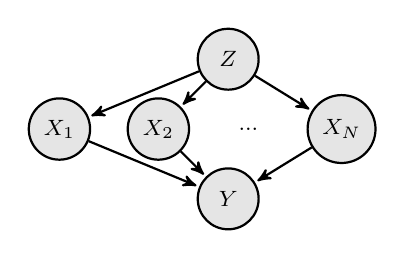
\begin{tikzpicture}[->,>=stealth',shorten >=1pt,auto,node distance=.45cm,
  thick,main node/.style={observed}, hidden/.style={empty},background rectangle/.style={fill=olive!45}]
%every node/.style={scale=0.6}
 %nodes
\node[main node](1){$X_{1}$};
\node[main node, right=of 1](2){$X_{2}$};
\node[hidden, right=of 2](3){$...$};
\node[main node, right=of 3](4){$X_{N}$};
\node[main node, below right=of 2](5){$Y$};
\node[main node, above right=of 2](6){$Z$};
 \path[every node/.style={font=\tiny}]
    (1) edge (5)
    	(2) edge (5)
    (4) edge (5)
    (6) edge (1) edge (2) edge (4);
\end{tikzpicture}
        \caption{Confounded graph}
        \label{fig:parallel_confounded} 
\end{figure}


We now compare the general algorithm with a range of standard bandit algorithms on the confounded graph in Figure \ref{fig:parallel_confounded}. All the variables are binary and the action space consists of the set of single variable interventions plus the do nothing action, $\calA = \set{\set{do(X_i = j)} \cup \set{do(Z = j)} \cup \set{do()}: 1\leq i \leq N,\; j \in \set{0,1}}$. We choose this setting because it generalises the parallel bandit, while simultaneously being sufficiently simple that we can compute the exact reward and interventional distributions for large $N$ (in general inference in graphical models is exponential in $N$). As before, we show the average regret over 10,000 simulations with error bars showing three standard errors. 

In Figure \ref{fig:simple_vs_m_general} we fix $N$ and $T$ and $P(Z=1) = .4$. For some $2 \leq N_1 \leq N$ we define 
\eq{
P(X_i = 1|Z = 0) &= \begin{cases} 0 & \text{ if } i \in \set{1,...N_1} \\ .4 & \text{ otherwise } \end{cases}\\
P(X_i = 1|Z = 1) &= \begin{cases} 0 & \text{ if } i \in \set{1,...N_1} \\ .65 & \text{ otherwise } \end{cases}
}
As in the parallel bandit case, we let $Y$ depend only on $X_1$, $P(Y|do(X_1=1)) = \frac{1}{2} + \epsilon$ and $P(Y|do(X_1=0)) = \frac{1}{2}-\epsilon'$, where $\epsilon' = \epsilon P(X_1=1) / P(X_1=0)$. The value of $N_1$ determines $m$ and ranges between $2$ and $N$. The values for the CPD's have been chosen such that the reward distribution is independent of $m$ and so that we can analytically calculate $\eta*$. This allows us to just show the dependence on $m$, removing the noise associated with different models selecting values for $\eta*$ with the same $m$ (and also worst case performance), but different performance for a given reward distribution. 

In Figure \ref{fig:simple_vs_T_general} we fix the model and number of variables, $N$, and vary the horizon $T$. $P(Z)$ and $P(X|Z)$ are the same as for the previous experiment.  
In Figure \ref{fig:simple_vs_T_misspecified} we additionally show the performance of Algorithm 1, but exclude actions on $Z$ from the set of allowable actions to demonstrate that Algorithm 1 can fail in the presence of a confounding variable, which occurs because it incorrectly assumes that $P(Y|do(X)) = P(Y|X)$. 
We let $P(Z) = .6$, $P(Y|\boldsymbol{X}) = X_7 \oplus X_N$ and $P(X|Z)$ be given by:

\eq{
P(X_i = 1|Z = 0) &= 
\begin{cases} 
.166 & \text{ if } i \in \set{1,..., 6} \\
.2 & \text{ if } i = 7 \\
.7 & \text { otherwise} 
 \end{cases}\\
 P(X_i = 1|Z = 1) &= 
\begin{cases} 
.166 & \text{ if } i \in \set{1,..., 6} \\
.8 & \text{ if } i = 7 \\
.3 & \text { otherwise} 
 \end{cases}\\
}

In this setting $X_7$ tends to agree with $Z$ and $X_N$ tends to disagree. It is sub-optimal to act on either $X_7$ or $X_N$, while all other actions are optimal. The first group of $X$ variables with $i \leq 6$ will be identified by the parallel bandit as the most unbalanced ones and played explicitly. All remaining variables are likely to be identified as balanced and estimated from observational estimates. The CPD values have been chosen to demonstrate the worst case outcome, where the bias in the estimates leads Algorithm 1 to asymptotically select a sub-optimal action.

\begin{figure}[H]
    \begin{subfigure}[t]{0.3\textwidth}
		\centering    
    		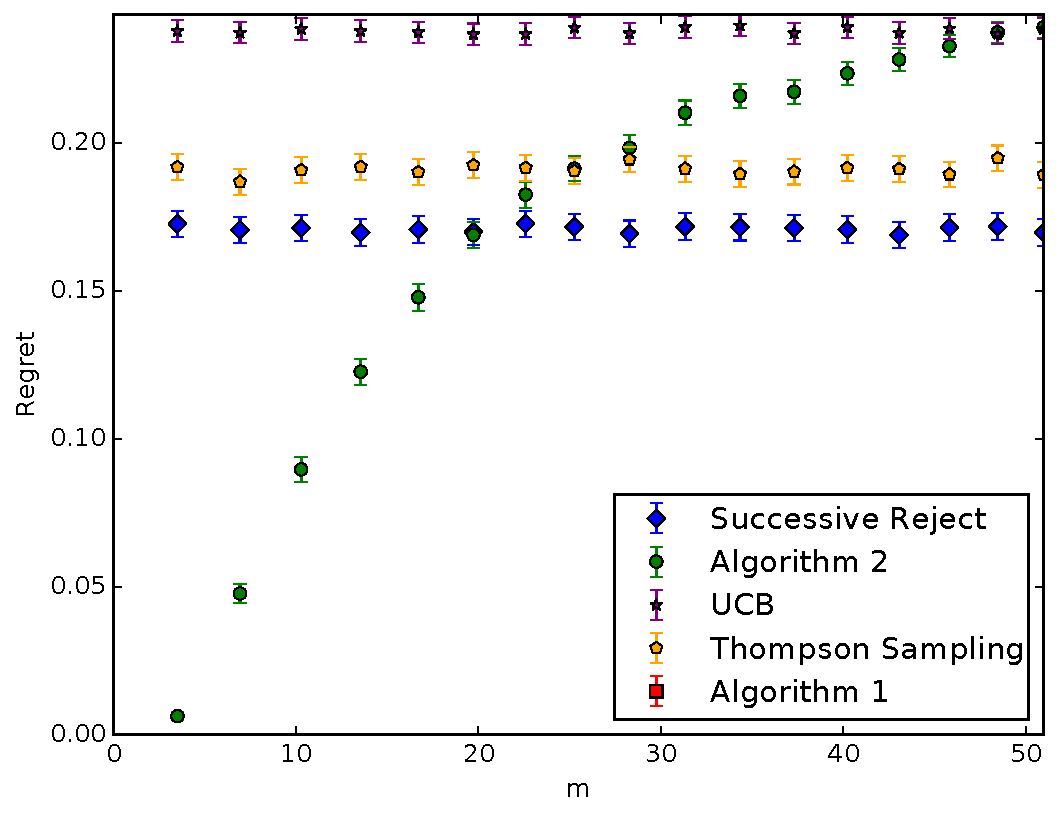
\includegraphics[width=\textwidth]{experiment4_20161023_2120.pdf}
    		\caption{Simple regret vs $m(\eta*)$ for fixed horizon $T=400$ and number of variables $N = 50$}
        \label{fig:simple_vs_m_general}
    \end{subfigure}\hfill
    \begin{subfigure}[t]{0.3\textwidth}
    		\centering
        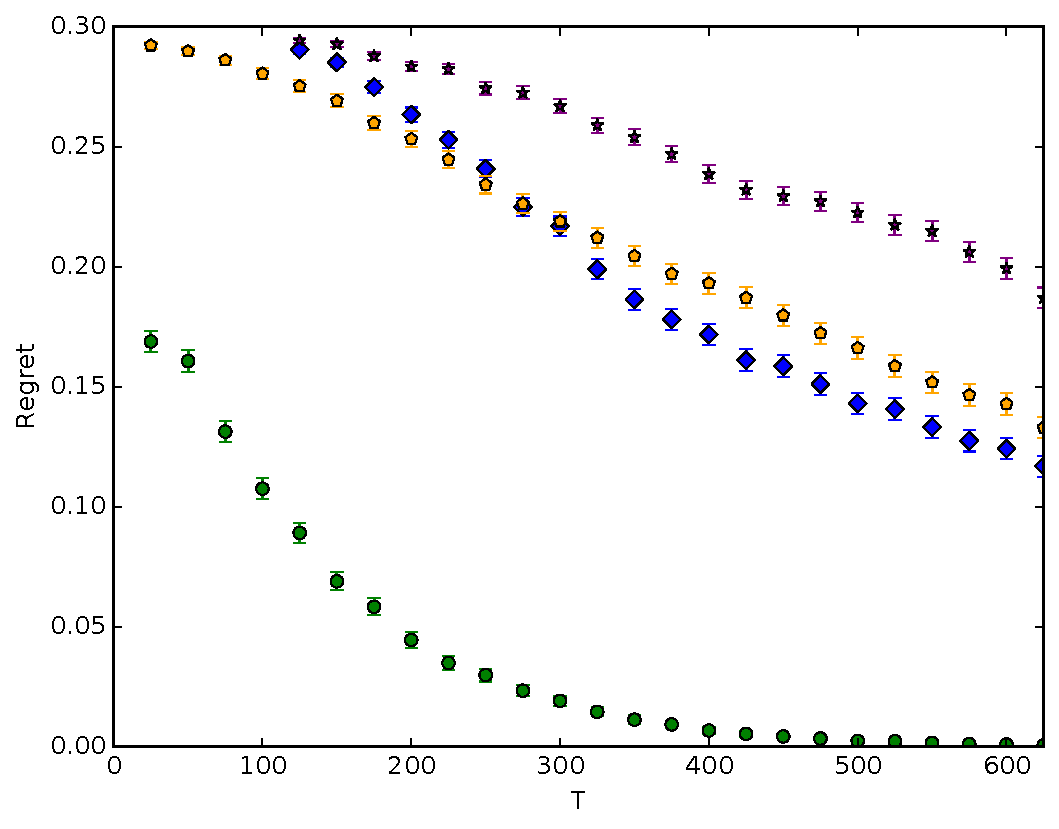
\includegraphics[width=\textwidth]{experiment7_20161020_1257.pdf}
    		\caption{Simple regret vs horizon, $T$, with $N = 50$ and $m(\eta*)=3.1$ }
        \label{fig:simple_vs_T_general}
    \end{subfigure}\hfill
    \begin{subfigure}[t]{0.3\textwidth}
    		\centering
    		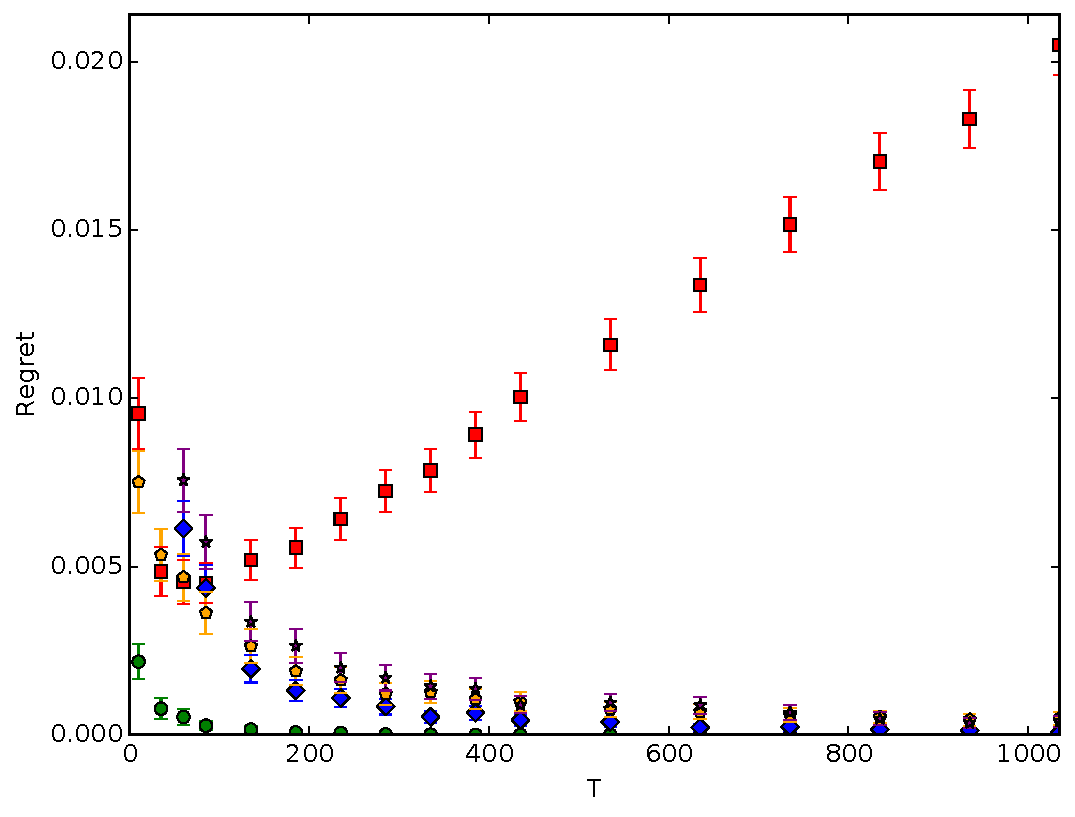
\includegraphics[width=\textwidth]{experiment5_20161023_2118.pdf}
    		\caption{Simple regret vs horizon, $T$, with $N = 21$, $m(\eta*)=4.3$ with no actions setting $Z$}
    		\label{fig:simple_vs_T_misspecified}
    \end{subfigure}
    \caption{Experimental results on the confounded graph}
    \label{fig:experiments_confounded}
\end{figure}

\subsection{Discussion \& Future work}

Algorithm~\ref{alg:general} for general causal bandit problems 
estimates the reward for all allowable interventions $a \in \calA$ over $T$ rounds by sampling and applying interventions from a distribution $\eta$.
Theorem~\ref{thm:general} shows that this algorithm has (up to log factors) simple regret that is $\smash{\mathcal O(\sqrt{m(\eta)/T)}}$ where 
the parameter $m(\eta)$ measures the difficulty of learning the causal model and is always less than $N$.
The value of $m(\eta)$ is a uniform bound on the variance of the reward estimators $\hat{\mu}_a$ and, intuitively, problems where all variables' values in the causal model ``occur naturally'' when interventions are sampled from $\eta$ will have low values of $m(\eta)$.

The main practical drawback of Algorithm~\ref{alg:general} is that both the estimator $\hat{\mu}_a$ and the optimal sampling distribution $\eta^*$ (\ie, the one that minimises $m(\eta)$) require knowledge of the conditional distributions $\Pn{a}{\parents{Y}}$ for all $a \in \calA$. In contrast, in the special case of parallel bandits, Algorithm~\ref{alg:simple} uses the $do()$ action to effectively estimate $m(\eta)$ and the rewards then re-samples the interventions with variances that are not bound by $\hat{m}(\eta)$.
Despite these extra estimates, Theorem~\ref{thm:lower} shows that this approach is optimal (up to log factors).Finding an algorithm that only requires the causal graph and lower bounds for its simple regret in the general case is left as future work.


\paragraph{Making Better Use of the Reward Signal}
Existing algorithms for best arm identification are based on ``successive rejection'' (SR) of arms based on UCB-like bounds on their rewards~\citep{Even-Dar2002}. In contrast, our algorithms completely ignore the reward signal when developing their arm sampling policies and only use the rewards when estimating $\hat{\mu}_a$. Incorporating the reward signal into our sampling techniques or designing more adaptive reward estimators that focus on high reward interventions is an obvious next step. This would likely improve the poor performance of our causal algorithm relative to the successive rejects algorithm for large $m$, as seen in Figure~\ref{fig:simple_vs_m}.

For the parallel bandit the required modifications should be quite straightforward. The idea would be to adapt the algorithm to essentially use successive elimination in the second phase so arms are eliminated as soon as they are provably no longer optimal with high probability. In the general case a similar modification is also possible by dividing the budget $T$ into phases and optimising the sampling distribution $\eta$, eliminating arms when their confidence intervals are no longer overlapping. Note that these modifications will not improve the minimax regret, which at least for the parallel bandit is already optimal. For this reason we prefer to emphasise the main point that causal structure should be exploited when available. Another observation is that Algorithm \ref{alg:general} is actually using a fixed design, which in some cases may be preferred to a sequential design for logistical reasons. This is not possible for Algorithm \ref{alg:simple}, since the $\vec{q}$ vector is unknown.


\paragraph{Cumulative Regret}
Although we have focused on simple regret in our analysis, it would also be natural to consider the cumulative regret. In the case of the parallel bandit problem we can slightly modify the analysis from \citep{wu2015online} on bandits with side information 
to get near-optimal cumulative regret guarantees. They consider a finite-armed bandit model with side information where in reach round the learner chooses an action and receives a Gaussian reward signal for all actions, but with a known variance that depends on the chosen action. In this way the learner can gain information about actions it does not take with varying levels of accuracy. The reduction follows by substituting the importance weighted estimators in place of the Gaussian reward. In the case that $\vec{q}$ is known this would lead to a known variance and the only (insignificant) difference is the Bernoulli noise model. In the parallel bandit case we believe this would lead to near-optimal cumulative regret,
at least asymptotically. 

%Their model assumes the rewards for all arms $a$ are Gaussian with mean $\mu_a$ and variance $\sigma^2_{ab}$ and that playing an arm $a$ will reveal a side observation $Y_{ab}$ of the reward for all arms $b$ distributed with mean $\mu_b$ and variance $\sigma^2_{ab}$.
%We can build a similar dependence structure with variances for a Bernoulli reward variable that is derived from the $\vec{q}$ vector of probabilities.
%\todom{Check this!}
%Even though the original results are for Gaussian rewards we believe the analysis will go through largely unchanged.

The parallel bandit problem can also be viewed as an instance of a time varying graph feedback problem \citep{Alon2015,Kocak2014}, where at each time step the feedback graph $G_t$ is selected stochastically, dependent on $\boldsymbol{q}$, and revealed after an action has been chosen. The feedback graph is distinct from the causal graph. A link $A \rightarrow B$ in $G_t$ indicates that selecting the action $A$ reveals the reward for action $B$. For this parallel bandit problem, $G_t$ will always be a star graph with the action $do()$ connected to half the remaining actions. However, \citet{Alon2015,Kocak2014} give adversarial algorithms, which when applied to the parallel bandit problem obtain the standard bandit regret. A malicious adversary can select the same graph each time, such that the rewards for half the arms are never revealed by the informative action. This is equivalent to a nominally stochastic selection of feedback graph where $\boldsymbol{q} = \boldsymbol{0}$. 

\cite{Lelarge2012} consider a stochastic version of the graph feedback problem, but with a fixed graph available to the algorithm before it must select an action. In addition, their algorithm is not optimal for all graph structures and fails, in particular, to provide improvements for star like graphs as in our case. \cite{Buccapatnam2014} improve the dependence of the algorithm on the graph structure but still assume the graph is fixed and available to the algorithm before the action is selected. 



\paragraph{Causal Models with Non-Observable Variables}
If we assume knowledge of the conditional \textit{interventional} distributions $\Pn{a}{\parents{Y}}$ our analysis applies unchanged to the case of causal models with 
non-observable variables. Some of the interventional distributions may be non-identifiable meaning we can not obtain prior estimates for $\Pn{a}{\parents{Y}}$ from 
even an infinite amount of observational data. Even if all variables are observable and the graph is known, if the conditional distributions are unknown, then Algorithm
\ref{alg:general} cannot be used. Estimating these quantities while simultaneously minimising the simple regret is an interesting and challenging open problem.

% For example, if we had access to a data set of \textit{experiments} in which the reward variable $Y$ was not available from which to build estimates of $P_a$.
% In this case, some conditional distributions may be non-identifiable. 
% The corresponding actions can be immediately added to the set $A$ prior to collecting any data. 
% We can then use the same algorithm as in the case where there are no latent variables, except that we will have to use the more general do-calculus rather than simply adjusting for the parents to write the expression for each action in terms of observational data.
% Combining our estimation techniques with insights from \citet{Bareinboim2015} for handling unobserved confounders would be worth investigation.


% More generally, assuming causal structure creates more complex types of side information, such as that shown in equation \ref{eq:estimation_transfer}. In this case, selecting one action does not fully reveal an alternate action but provides some information towards an estimate. The quality of the estimate notably depends not only on the number of times that action was selected. For example, to get a good estimate for $X_1 = 1$ by intervening on $X_2$ requires us to sample both $X_2=0$ and $X_2=1$, in proportions dependent on $q_2$. This more complex side information does not fit within the graph feedback framework.


\paragraph{Partially or Completely Unknown Causal Graph}
A much more difficult generalisation would be to consider causal bandit problems where the causal graph is completely unknown or known to be a member of class of models.
The latter case arises naturally if we assume free access to a large observational data set, from which the Markov equivalence class can be found via causal discovery techniques. 
Work on the problem of selecting experiments to discover the correct causal graph from within a Markov equivalence class~\cite{Eberhardt2005,eberhardt2010causal,hauser2014two,Hu2014b} could potentially be incorporated into a causal bandit algorithm.
In particular, \citet{Hu2014b} show that only $\bigo{\log \log n}$ multi-variable interventions are required on average to recover a causal graph over $n$ variables once purely observational data is used to recover the ``essential graph''.
Simultaneously learning a completely unknown causal model while estimating the rewards of interventions without a large observational data set would be much more challenging.

\subsection{Proofs}

\chapter{List of software programs for causal inference}

\begin{itemize}
\item Pcalg. A library in R that implements ...
\item Tetrad.
\item There has to be a library for the bayesian trees thing
\item Linear regression (you can do this anywhere)

\end{itemize}

\chapter{Causality \& Interpretability}

\chapter{Causality \& Fairness}

As machine learning is incorporated into decision making systems that have fundamental impacts on people’s lives, such as in employment, criminal justice, health and financial services, there are increasing concerns over transparency and fairness \cite{WMD, etc}. Realisation that machine learning algoithms can be inherit biases from the data we feed into them and the choices those building them make about what variables to enclude, etc. 

The European Union’s General Data Protection Regulation \cite{Goodman2016}\todo{check}, due to come into effect in 2018, requires that people can obtain "meaningful information about the logic involved" in an automated decision process . It also stipulates that such decisions should not be based on special categories of personal data (related to ethnicity, political and religions affiliation or sexuality) unless there "suitable measures" to safeguard individual interests. A key concern is discrimination against disadvantaged groups. 

Discrimination is frequently defined in terms of either disparate treatment- treating otherwise similar individuals differently on the basis of a protected attribute such as race or gender, or disparate impact - a process that yields a significant difference in outcome between groups. We consider how the notions of disparate treatment and impact may be formalised and the implications of how this is done for machine learning. We examine the overlap between the motivations for interpretable and causal models, especially with respect to assessing fairness. We look at how causal models mitigate some of the trade-offs between transparency and predictive accuracy and we examine to what extent the causal relationship between an attribute, any protected attributes and the outcome of interest is relevant to assessing the impact on fairness of its inclusion in a machine learning model.

The lack of part-time work in tech could be argued to constitute indirect discrimination against women. 
A fear that advertising themselves as supporting flexible working options would attract candidates who lacked drive and ambition.
Cultural bais that favours those driven by monitary ambition against those 


Stability - a non causal model can't tell us about a simple do type opperation on  a single variable. 

More broadly, we could draw a model representing the system now that could tell us the result of an intervention on a particular variable (such as setting gender), but the system itself could change (for example with customer preferences). There is a notion that a true causal model should be invariant for all time.

Connection to Simpson's paradox. But what should we condition on? \cite{Romie2010} argue that looking at the department level is the correct viewpoint, since this the point at which hiring decions were made. However, it could be argued that if one department was attracting a large number of higher quality candidates, the overall size of that deparmtment should be higher and that the results seen at Berkley reflected a bias in favour of male dominated fields. 

Different measures of discrimination - is there a difference between groups (after conditioning on xxx)

To understand how we measure and penalise discrimination, we need to take a step back and ask what are the underlying motivations for fairness?

These differences in underlying cause suggest differences in the approach we should take to remedy them.  

\section{How does discrimination arise in ML models}
\begin{itemize}
\item bias in historical decisions fed in as training data
\item selection bias in input data, due to deliberate or implicit discrimination such as stop and search
\item deliberate manipulation on the part of the person building the model.
\item The hardest case is historical disadvantage, creating genuine differences between relevent attributes of groups.
\item in bias in the label - what happens if you hire minorities but then your staff treat them badly and as a result they underperform or leave.  
\end{itemize}

\section{Defining Descrimination}

Define discrimination in terms of causal effect of protected variable in decision making process. 

\cite{Romei2012} note the relevence of causal inference on discrimintation analysis.

“the central question in any employment- discrimination case is whether the employer would have taken the same action had the employee been of 7A recurring problem known as the omitted-variable bias.
A multidisciplinary survey on discrimination analysis 9
a different race (age, sex, religion, national origin etc.) and everything else had been the same” (Carson v. Bethlehem)


Let us mathematically define disparate treatment and disparate impact with respect to a statistical model. We will focus on discrete variables for notational simplicity. Assume we have an outcome of interest $Y$, protected attributes $X$, other covariates $Z$ and a (potentially stochasitic) model $f$ that maps $\{x, z\}$ to $y_f \in Y$. For a given model $f$, we have a distribution over the predicted outputs given the inputs, $\P{Y_f|X,Z}$
\vspace{.2cm}
\begin{definition}{Disparate Impact}: A model, $f$, that produces a predictive distribution $\P{Y_f|X,Z}$ has disparate impact if the marginal distribution over the predicted outcome, $Y_f$, depends on a protected attribute.
\eqn{
\exists \set{x_1,x_2} \subset X: \sum_z{\P{Y_f|Z,x_1}\P{Z|x_1}} \neq \sum_z{\P{Y_f|Z,x_2}\P{Z|x_2}}
}
\end{definition}

\begin{definition}{Disparate Treatment}: A model yeilds disparate treatment if people with identical attributes (excuding protected attributes) are treated differently. 
\eqn{
\P{Y_f|Z,X} \neq \P{Y_f|Z}
}
\end{definition}

Avoiding treating people differently purely on the basis of attributes such as ethnicity and gender and avoiding large differences in important outcomes such as education and income between such groupings both seem like desirable goals. Unfortunately, in general, they conflict with one another, see theorem \ref{thm:disparate_conflict}. Any variable we might wish to aviod discriminating on will be correlated to some other measurable covariate $Z$, making it impossible to avoid both disparate treatment and disparate impact. 
\vspace{.2cm}
\begin{theorem} 
\label{thm:disparate_conflict}
Disparate impact and disparate treatment conflict. Given covariates $Z$ and protected attributes $X$, a model, $f$, cannot be fair with respect to both disparate impact and disparate treatment unless $\P{Z|X} = \P{Z}$.
\begin{proof} Assume $f$ yeilds no different treatment, then $\P{Y_f|Z,X} = \P{Y_f|Z}$. If we additionally assume no disparate impact, $\sum_z{\P{Y_f|Z}\P{Z|x_1}} = \sum_z{\P{Y_f|Z}\P{Z|x_2}} \;\; \forall \set{x_1,x_2}\subset X$. This holds if and only if $\P{Z|x_1} = \P{Z|x_2} \;\; \forall \set{x_1,x_2} \implies \P{Z|X} = \P{Z}$
\end{proof} 
\end{theorem}  

Further issues.


Disparate treatment, with respect to an observed set of variables $Z$, can be trivially avoided by excluding protected attributes from the training data. 

Problems:
\begin{itemize}
\item Disparate impact and disparate treatment conflict
\item 
\end{itemize}



\section{Addressing discrimination}

Ommititting the protected attribute from the model can increase disparate impact, even if the protected attribute is negatively correlated with the outcome. 


\textit{Disparate treatment} can be trivially avoided by excluding the protected variable from the model. However, this is deeply unsatisfying given the presence of proxy variables and can increase bias (figure \ref{fig:recidivism})

Avoiding \textit{disparate impact} may be be expensive in terms of predictive accuracy and/or require \textit{disparate treatment}. 

\begin{figure}[H]
\caption{Proxies}
\label{fig:recidivism}
	\centering    
          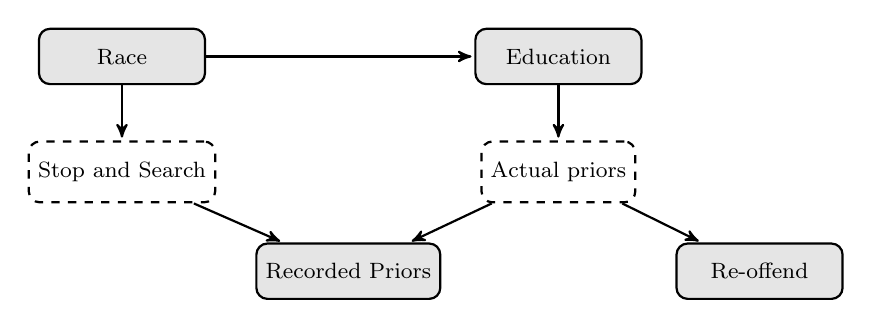
\begin{tikzpicture}[->,>=stealth',shorten >=1pt,auto,node distance=.7cm,
  thick,main node/.style={observedrect}, lt/.style={latentrect} , hidden/.style={empty},background rectangle/.style={fill=olive!45}]
 %nodes
\node[lt](1){Actual priors};
\node[main node, below left=of 1](2){Recorded Priors};
\node[main node, below right=of 1](3){Re-offend};
\node[lt, above left=of 2](4){Stop and Search};
\node[main node, above=of 4](5){Race};
\node[main node, above=of 1](6){Education};
 \path[every node/.style={font=\tiny}]
    (1) edge (2) edge (3)
    (4) edge (2)
    (5) edge (4) edge (6)
    (6) edge (1);
\end{tikzpicture}
\end{figure}


\begin{itemize}
\item There is an additional connection between causality and fairness, that arises when you know that there is a bias in the data and wish to correct for it. In causality, it may be due to selection bias or a confounding variable. In fairness, it may be due to historical disadvantage. In both cases we may have theory that tells us the direction or scale of an effect. Ie, we know that race itself has no inherent effect on outcomes such as criminality and education. If you have a data set and a collection of such priors, where the data contradicts these priors due to data bias. How do you best make decisions based on that data? 
\end{itemize}


human decicion making can evolve. 

The vaugeness inherent in writing laws in natural language allows for them to be re-interpreted. 

There is a lack of diversity in models. (although radomness is in fact inherent in many) - could one leverage this? - you would need an estimate of the probability the model would have assigened each instance to a particular group. 

Only humans can provide the ethics




\chapter{Causality in Marketing}
Assessing the impact of marketing spend is becoming increasingly important to industry. Billions of dollars \cite{XXX} are spent each year and new marketing channels and opportunities are opening up at an unprecedented rate. 

There are three key approaches to assessing the impact of marketing in the literature. 

The first is to look for correlations across companies on metrics such as how much they spend on marketing \ref{}, how confident they are about their ability to market effectively \ref{} or how important the marketing team is perceived to be within the organisation with indicators of the health of the company such as sales, revenue or market capitalisation. Unfortunately is is very difficult to avoid potential major confounders with this approach. Are businesses large and successful because of their capable marketing teams or can they afford to hire capable marketers because they have sufficient profits available to do so. 

\section{Attribution}
The second is attribution. The goal in this case is to attribute each sale to a specific (or set of specific) advertisements that the customer was exposed to. This approach is the primary way of measuring the success of digital advertising strategies such as search, display, and online video ads. The most frequent model is last-click attribution. In which the last ad the customer was presented with before they made their purchase is assumed to have caused that sale. A central criticism of attribution is that it is not measuring incremental sales. Each sales is assumed to be a consequence of some form of advertising for those customers who saw (however briefly) some form of advertisement. Of course in reality many of these customers may have made a purchaser regardless of the advertising material to which they were exposed. 

System designed to optimise metrics such as click through or conversion rate can do so either by learning how to change the consumers preferences (by serving them the perfect ad at the ideal time) or by learning who was most likely to buy anyway. It seems likely that much of the improve mt in click through rates due to the application of sophisticated machine learning algorithms is being driven by the latter. Unfortunately, this does nothing for the bottom line of industry (except for those involved in serving ads). 


\section{Econometric Modelling}
The final key plank businesses apply to estimate how effective their marketing are econometric or mixed media models. These models

In practise these models are typically time series regression models, fitting some measure of sales against marketing spend (by marketing channel, ie TV, radio, search, digital display etc) and other key variables such as pricing, competitor spend and pricing and indicators of the health of the economy and demand for the product in question.

The models may also include non-linear transformation of the marketing inputs to represent saturation and decay of time of effects. They may also consider the interaction between media channels and other business levers such as pricing.  

The objective of these models is to obtain results that are comparable across channels such that the optimal mix of media can be selected. 

The key

\chapter{Conclusions (1000 words)}

\section{Open questions}
\paragraph{Cycles} - a huge issue. Not covered by Pearl,Rubin etc. 

Places to look, statistical control theory, etc. any interesting papers along these lines?

In the discrete case,
Fung and Crawford (1990) have recently proposed a fast algorithm for constructing an
independence graph from discrete data. We have not tested their procedure as a processor for
the PC algorithm. (COPIED FROM SPRITES)


\bibliographystyle{apalike}% Select the citation style e.g. ieeetr
\bibliography{../library}% write the directory to the .bib file
\end{document}




